\documentclass[12pt,UTF8]{ctexart}
\usepackage{ctex,amsmath,amssymb,geometry,fancyhdr,bm,amsfonts,mathtools,extarrows,graphicx,url,enumerate,xcolor,float,multicol,wasysym}
\usepackage{subfig}
\allowdisplaybreaks[4]
% 加入中文支持
\newcommand\Set[2]{\left\{#1\ \middle\vert\ #2 \right\}}
\newcommand\Lim[0]{\lim\limits_{n\rightarrow\infty}}
\newcommand\LIM[2]{\lim\limits_{#1\rightarrow#2}}
\newcommand\Ser[1]{\sum_{n=#1}^\infty}
\newcommand{\SER}[2]{\sum_{#1=#2}^\infty}
\newcommand{\Int}[4]{\varint\nolimits_{#1}^{#2}#3\mathrm d#4}
\newcommand{\aIInt}[1]{\iint\limits_{#1}}
\newcommand{\IInt}[3]{\iint\limits_{#1}#2\mathrm d#3}
\newcommand{\varIInt}[4]{\iint\limits_{#1}#2\mathrm d#3\mathrm d#4}
\newcommand{\IIInt}[3]{\iiint\limits_{#1}#2\mathrm d#3}
\newcommand{\varIIInt}[5]{\iiint\limits_{#1}#2\mathrm d#3\mathrm d#4\mathrm d#5}
\newcommand{\LInt}[3]{\varint\nolimits_{#1}#2\mathrm d#3}
\newcommand{\LOInt}[3]{\varoint\nolimits_{#1}#2\mathrm d#3}
\newcommand{\LLInt}[4]{\varint\nolimits_{#1}\nolimits^{#2}#3\mathrm d#4}
\newcommand{\BLInt}[2]{\varint\nolimits_{#1}#2}
\newcommand{\varBLInt}[3]{\varint\nolimits_{#1}\nolimits^{#2}#3}
\newcommand{\BLOInt}[2]{\varoint\nolimits_{#1}#2}
\newcommand{\SIInt}[3]{\iint\limits_{#1}#2\mathrm d#3}
\newcommand{\md}[1]{\mathrm d#1}
\newcommand{\BSIInt}[2]{\iint\limits_{#1}#2}
\newcommand{\pp}[2]{\frac{\partial #1}{\partial #2}}
\newcommand{\ppx}[1]{\frac{\partial #1}{\partial x}}
\newcommand{\ppy}[1]{\frac{\partial #1}{\partial y}}
\newcommand{\ppz}[1]{\frac{\partial #1}{\partial z}}
\newcommand{\varppx}[1]{\frac{\partial}{\partial x} #1}
\newcommand{\varppy}[1]{\frac{\partial}{\partial y} #1}
\newcommand{\varppz}[1]{\frac{\partial}{\partial z} #1}
\newcommand{\BSOIInt}[2]{\oiint\limits_{#1}#2}
\newcommand{\me}[0]{\mathrm e}
\geometry{a4paper,scale=0.80}
\pagestyle{fancy}
\rhead{多元函数积分学(3)}
\lhead{基础习题课期末复习}
\chead{微积分B(2)}
\begin{document}
\setcounter{section}{7}
\section{三重积分的计算}
\noindent
\subsection{复习计划}
\begin{figure}[H]
\begin{center}
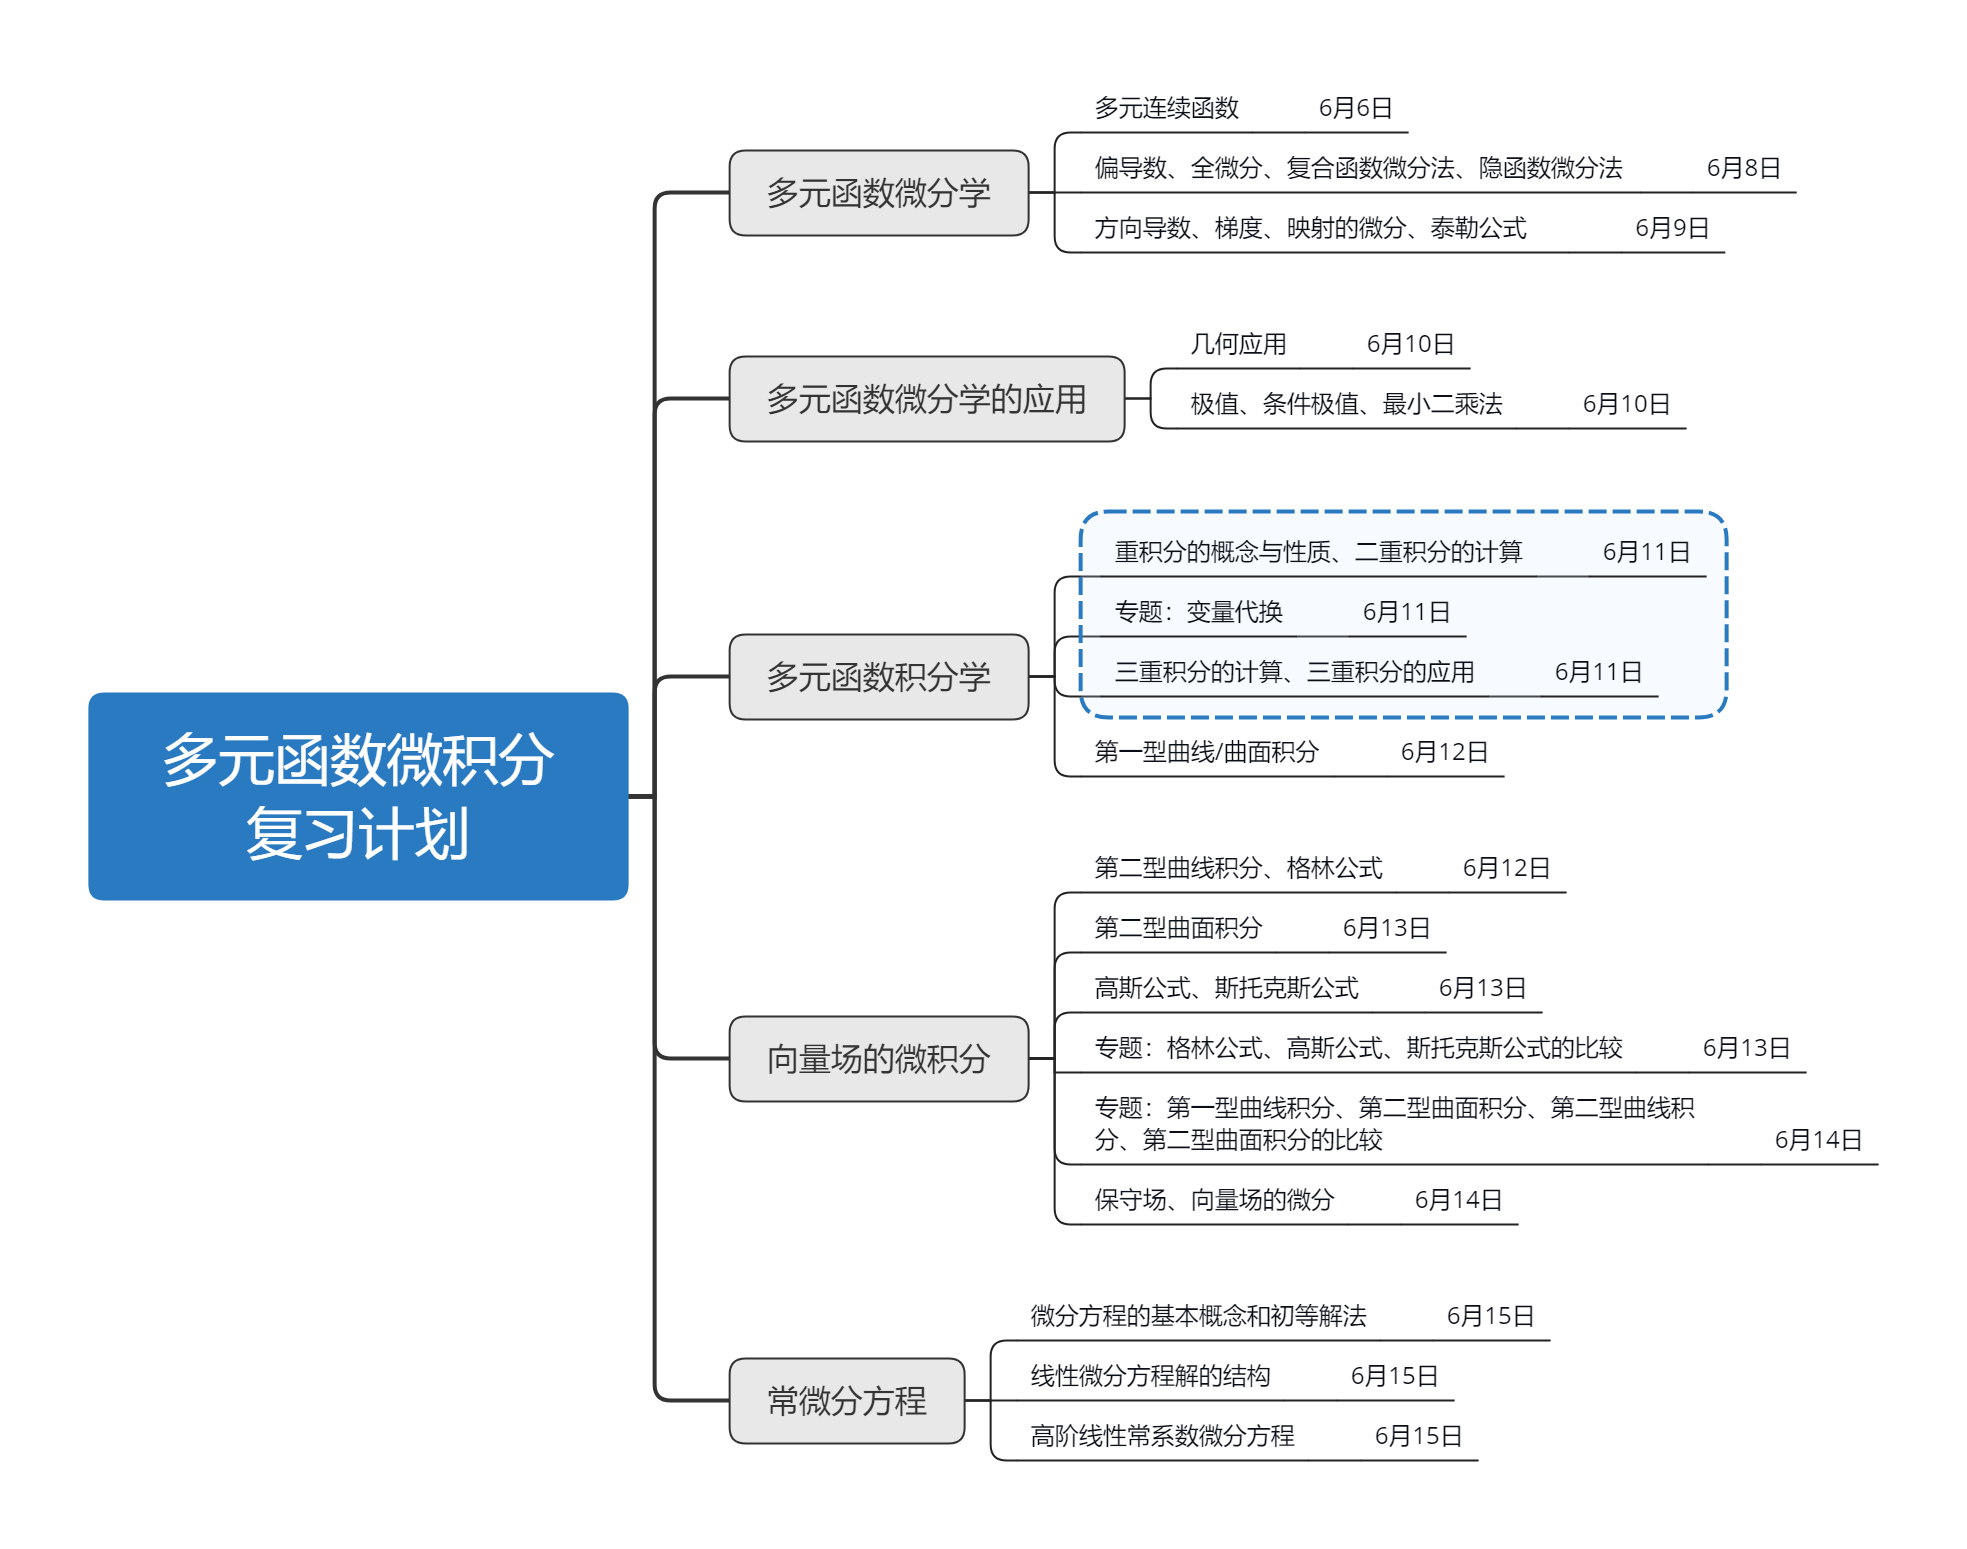
\includegraphics[height=0.5\textheight]{Figures20190611/plan.png}
\end{center}
\end{figure}
\subsection{知识结构}
\begin{figure}[H]
\begin{center}
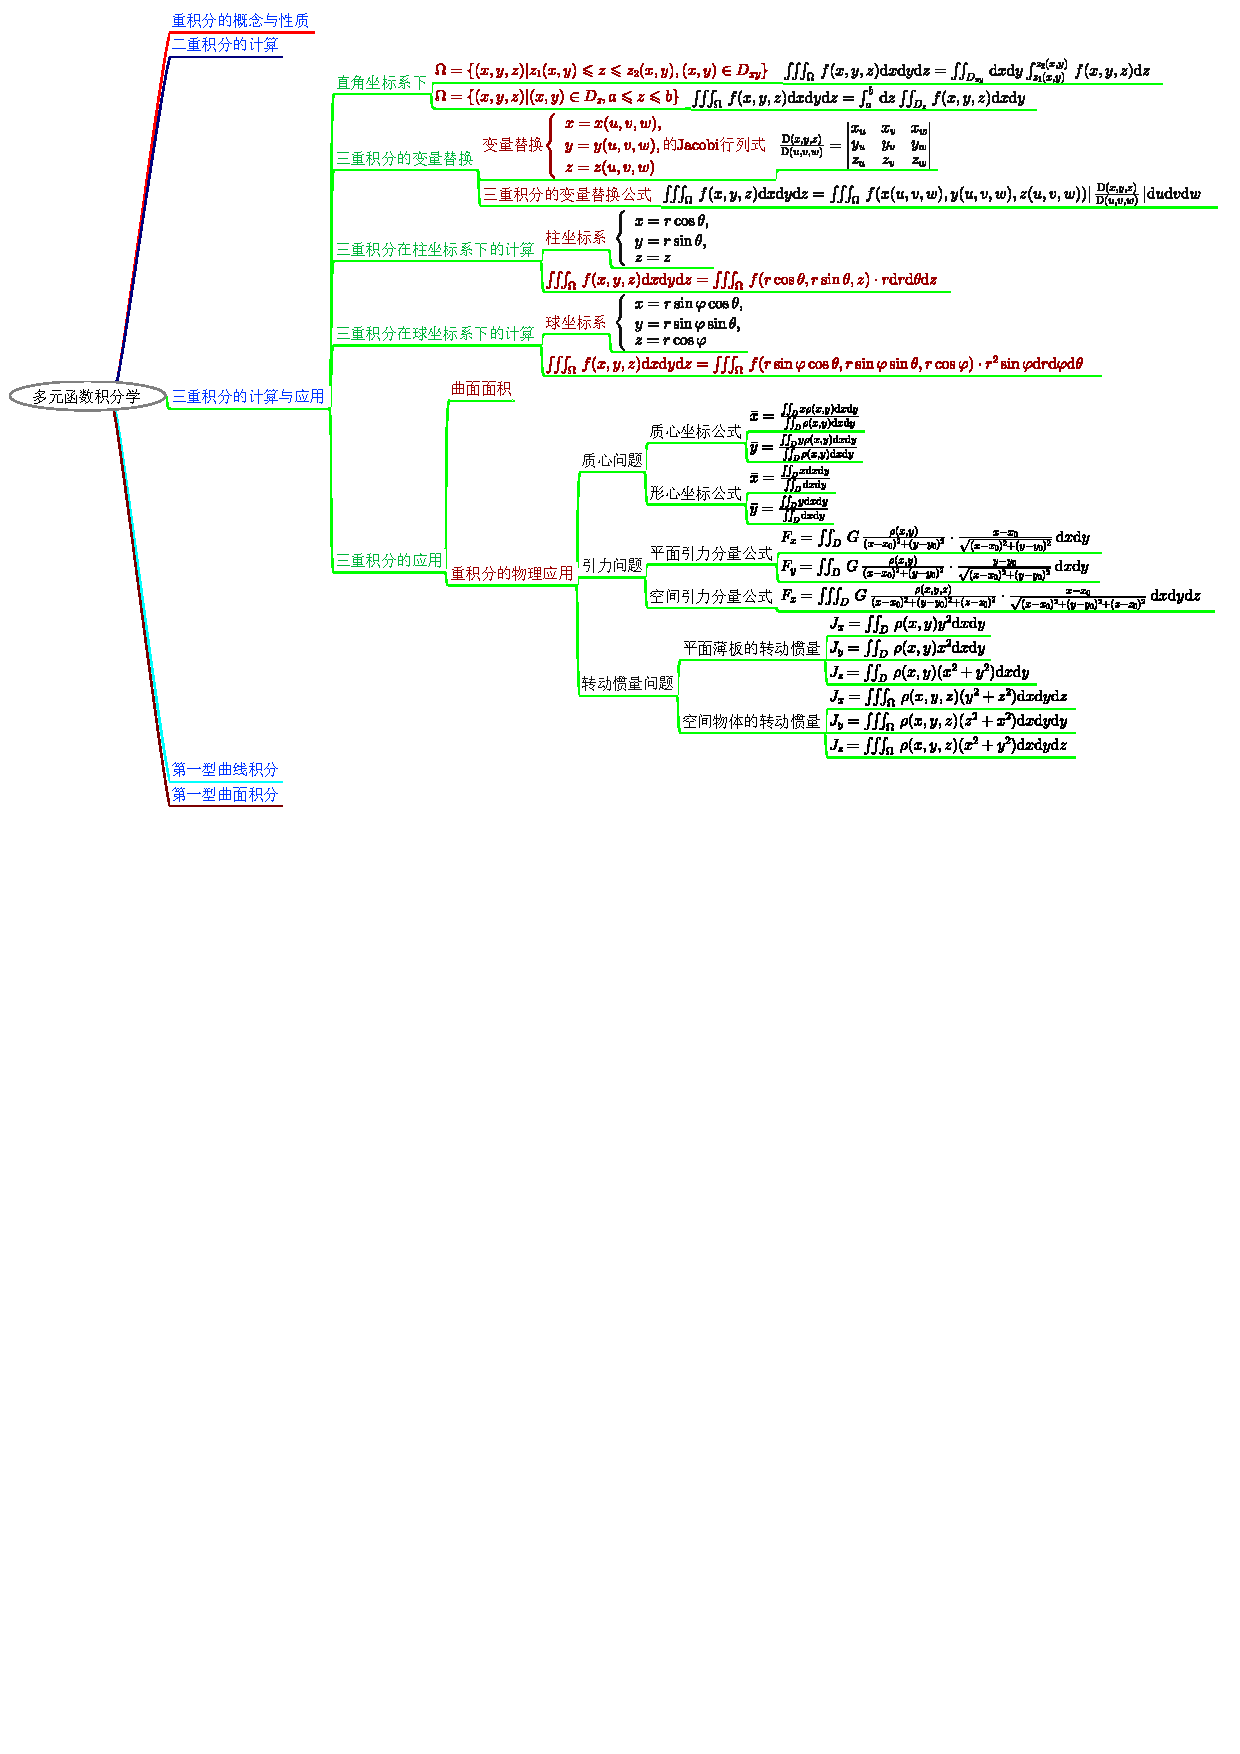
\includegraphics[height=0.9\textheight,angle=0]{20190611-2.pdf}
\end{center}
\end{figure}
\subsection{重要图示}
\begin{enumerate}
\item直角坐标系下的三重积分化为三次积分.
\begin{figure}[H]
\begin{center}
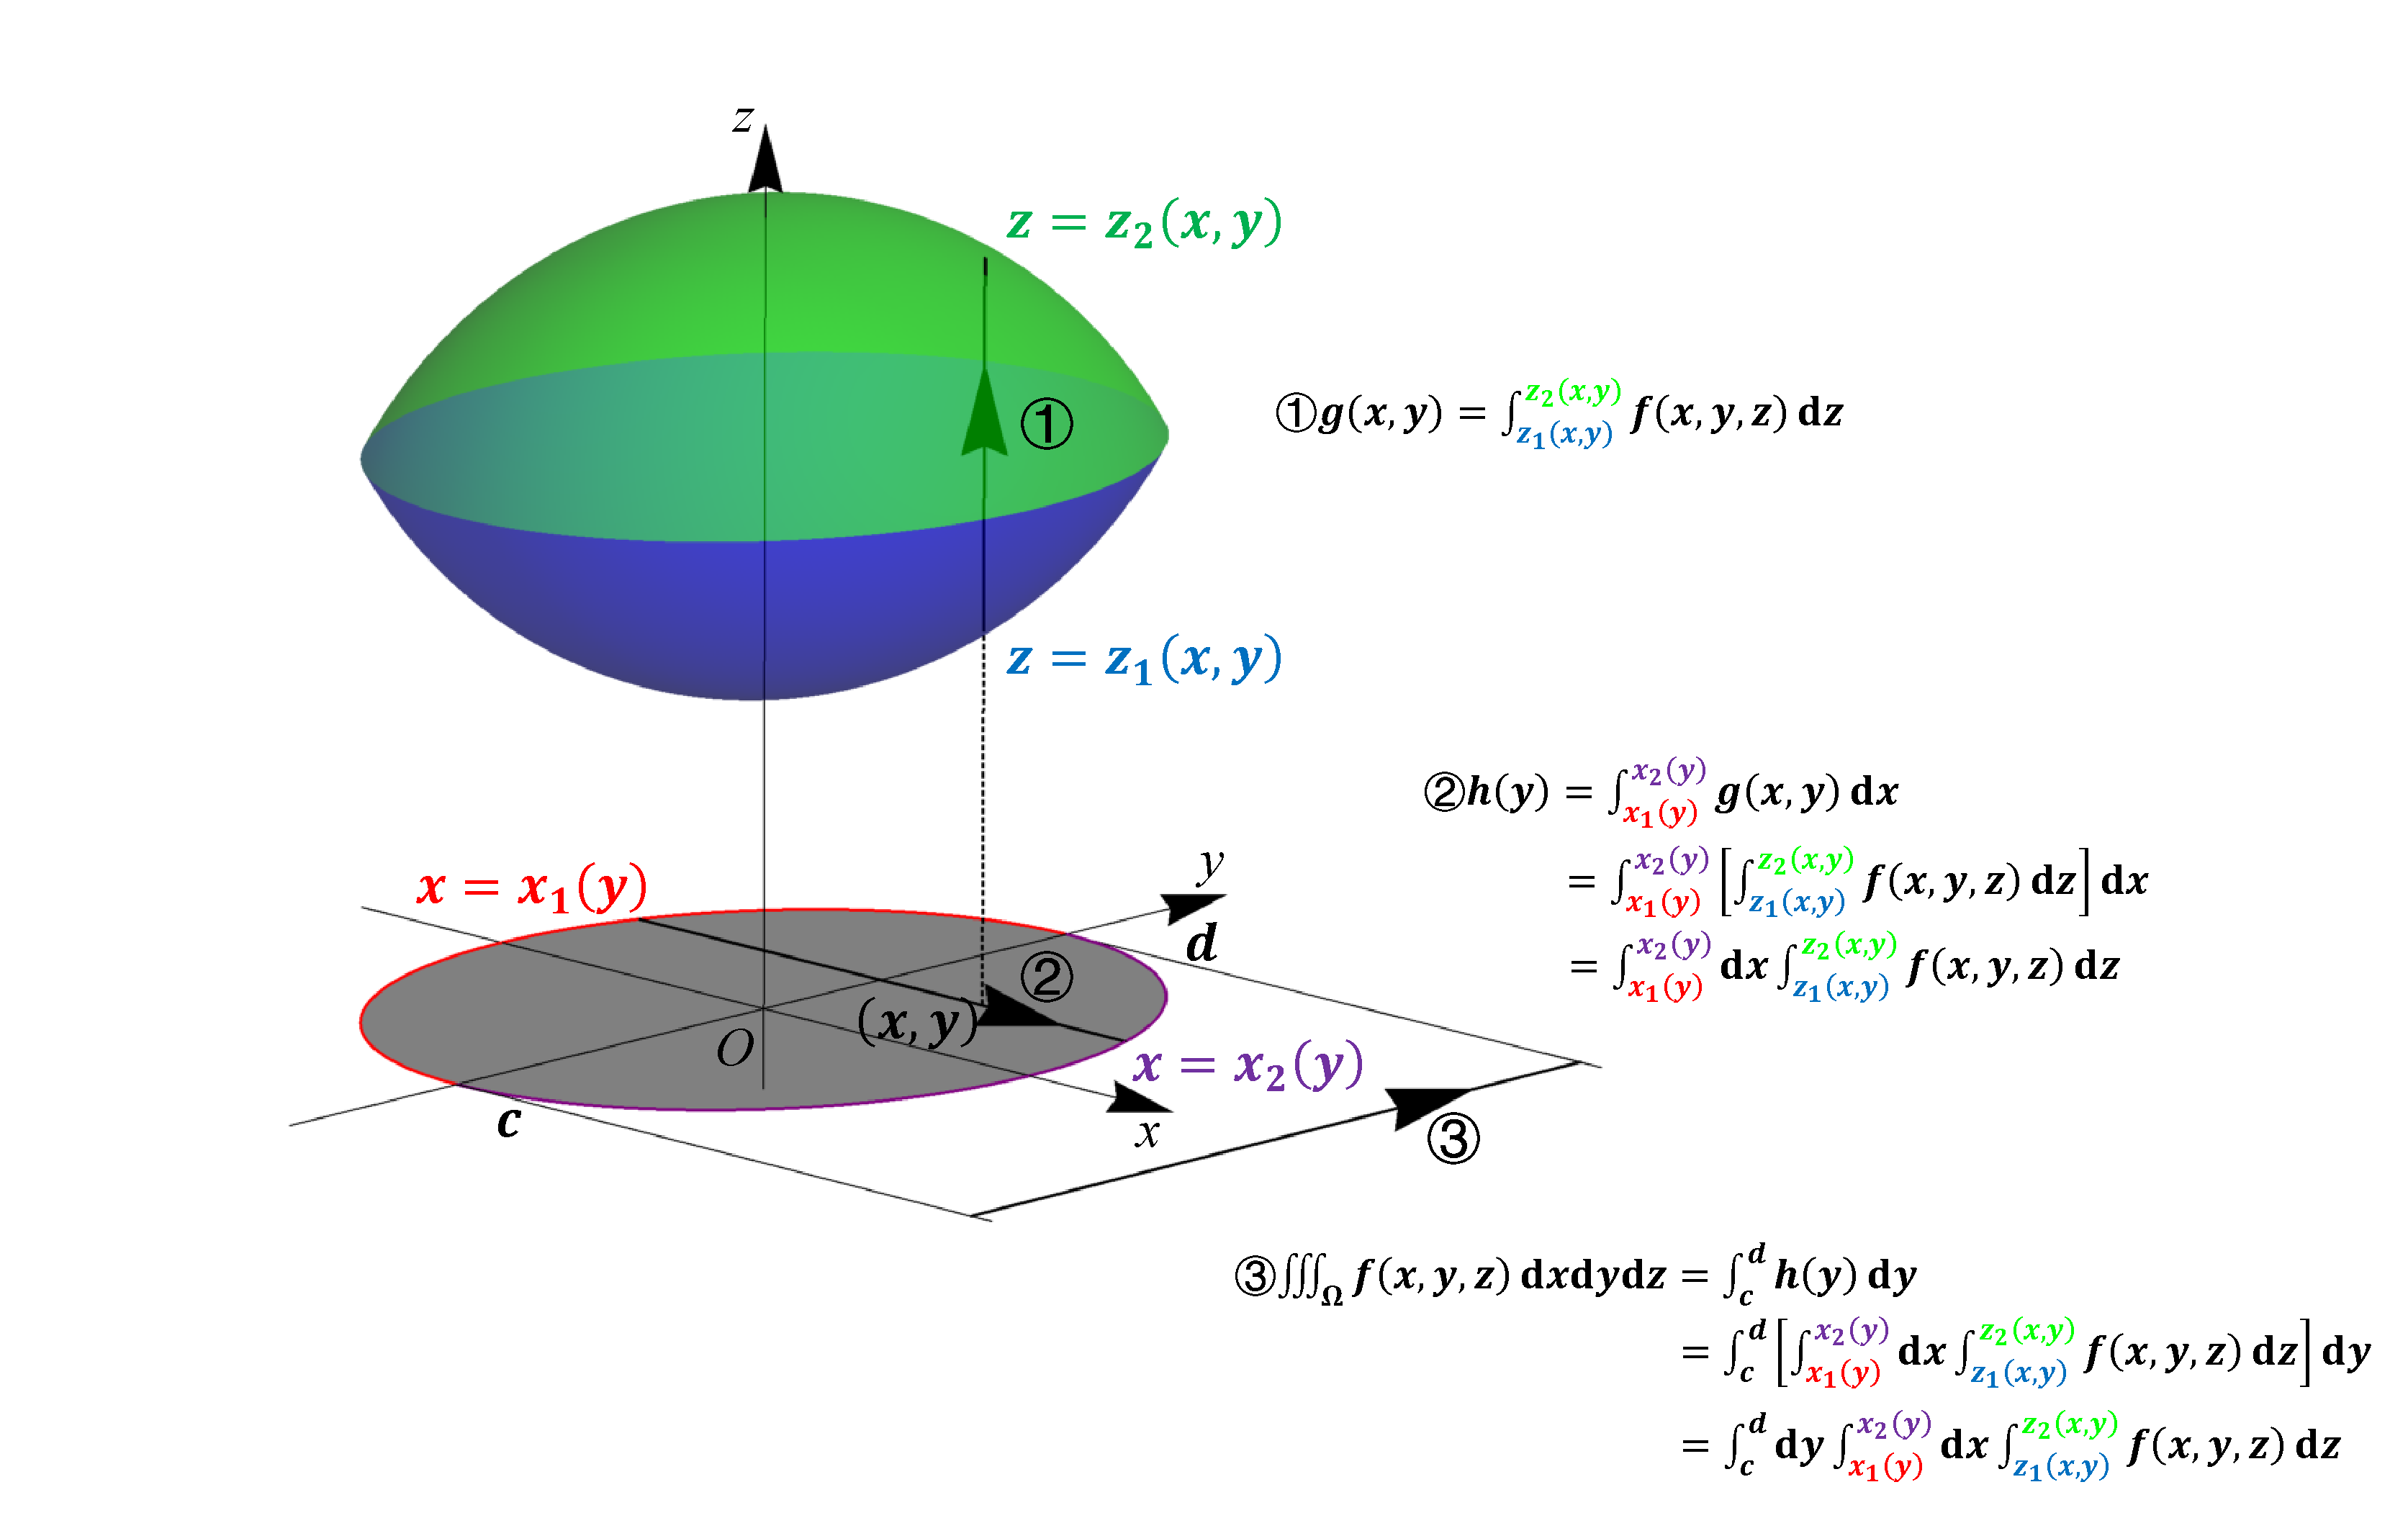
\includegraphics[height=0.5\textheight,angle=0]{Figures20190611/D2M.pdf}
\end{center}
\caption{直角坐标系下的三重积分化为三次积分}
\end{figure}
\item直角坐标系下的三重积分化为先二重积分后定积分的累次积分.
\begin{figure}[H]
\begin{center}
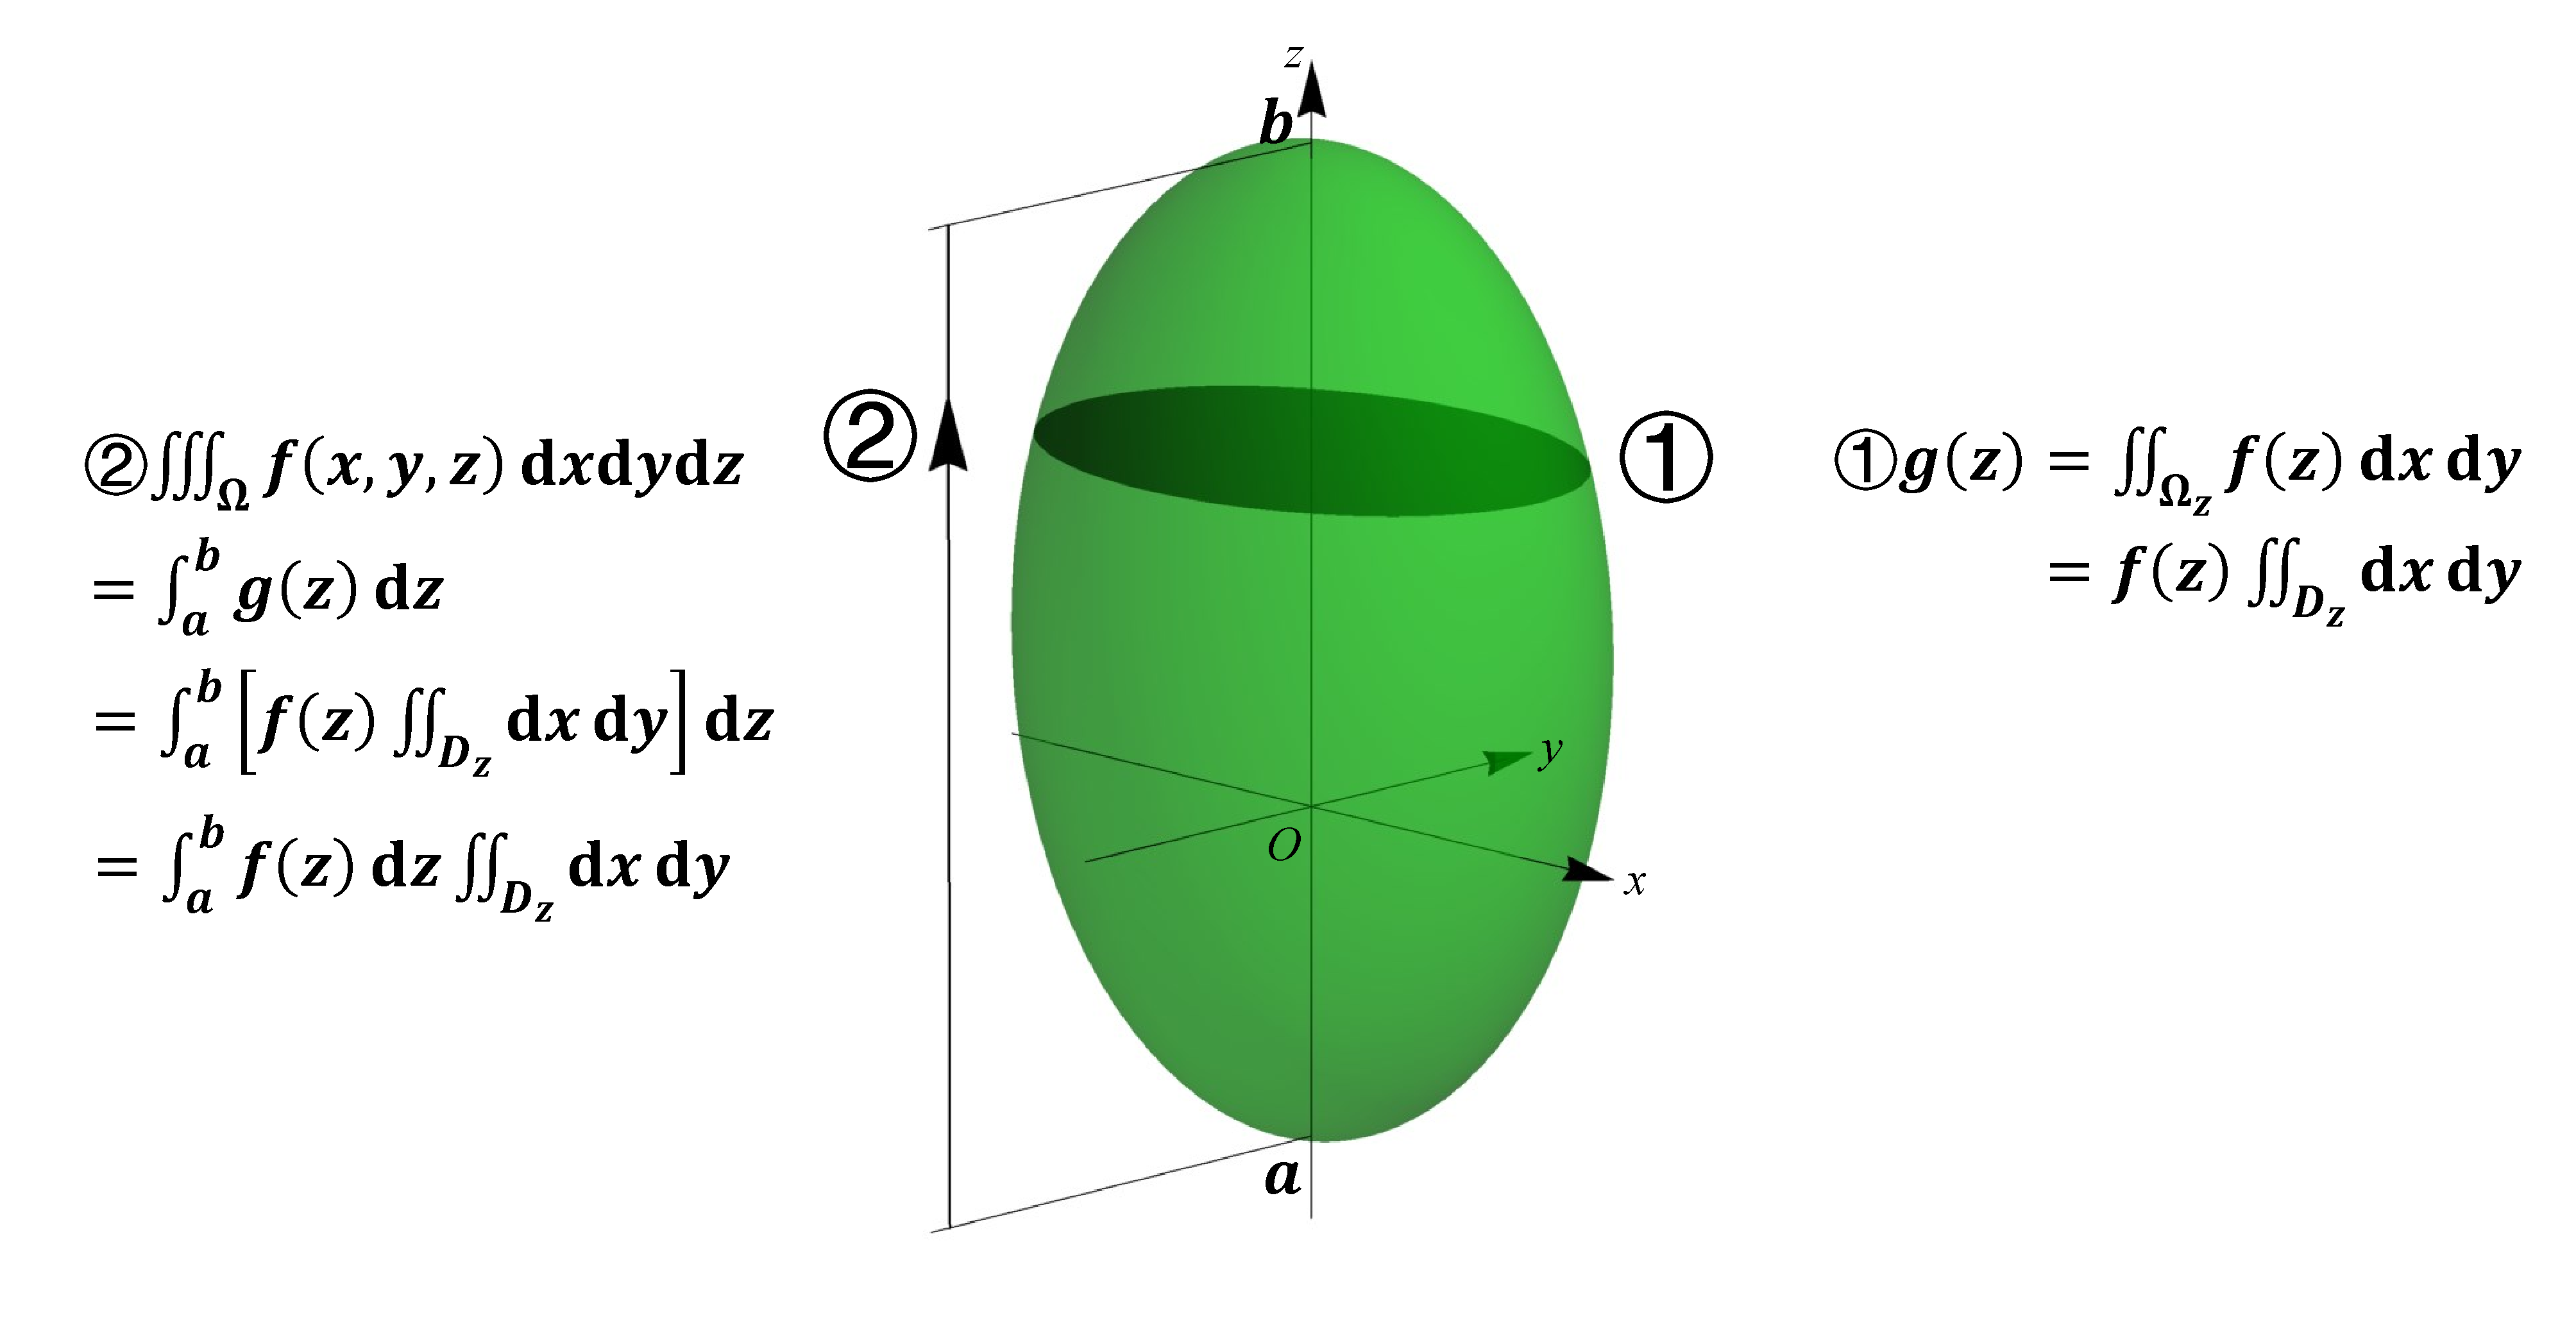
\includegraphics[height=0.3\textheight,angle=0]{Figures20190611/M2D.pdf}
\end{center}
\caption{直角坐标系下的三重积分化为先二重积分后定积分的累次积分}
\end{figure}
\item三重积分在柱坐标系下的计算.
\begin{figure}[H]
\begin{center}
\includegraphics[height=0.4\textheight,angle=0]{Figures20190611/pillar.pdf}
\end{center}
\caption{三重积分在柱坐标系下的计算}
\end{figure}
\item三重积分在球坐标系下的计算.
\begin{figure}[H]
\begin{center}
\includegraphics[height=0.3\textheight,angle=0]{Figures20190611/sphere.pdf}
\end{center}
\caption{三重积分在球坐标系下的计算}
\end{figure}
\end{enumerate}
\subsection{习题分类与解题思路}
\begin{enumerate}
\item直角坐标系下交换三重积分顺序.
【如习题12.4中的1., 6.】
\item直角坐标系下的三重积分化为先二重积分后定积分的累次积分. 此时被积函数只与$x,y,z$之一有关. 先化为二重积分,求出垂直于$x,y$或$z$轴的截面面积,该截面面积是$x,y,z$之一的函数,然后求出该被积函数与截面面积乘积的定积分.

【如习题12.4中的2., 6.】
\item柱坐标计算三重积分. 积分域在任意坐标面上的投影为圆形区域时可用柱坐标计算三重积分.

【如习题12.4中的3., 5., 6., 7., 8., 13., 14.(1), 19., 第12章补充题中的9.】
\item球坐标计算三重积分. 积分域含有球面时可用球坐标计算三重积分.

【如习题12.4中的4.(1), 6., 14.(2)】
\item利用对称性简化计算.

【如习题12.4中的4.(2), 8., 第12章补充题中的10.】
\item三重积分的变量替换.

【如习题12.4中的15.】

\item三重积分的物理应用. 包括重心(质心、形心)的计算、转动惯量的计算、引力的计算.

【如习题12.4中的16., 17., 18., 第12章补充题中的2., 3.】

\item其他类型的题目.

【习题12.4中的10.需要特殊的技巧,大家可以做一个积累.】

【习题12.4中的11., 12.为用二重积分求平面图形的面积.】

\end{enumerate}
\subsection{习题12.4解答}
\begin{enumerate}
\item求$I=\Int01{}x\Int0x{}y\Int0y{\frac{\sin z}{(1-z)^2}}z$的值.

\begin{figure}[H]
\begin{center}
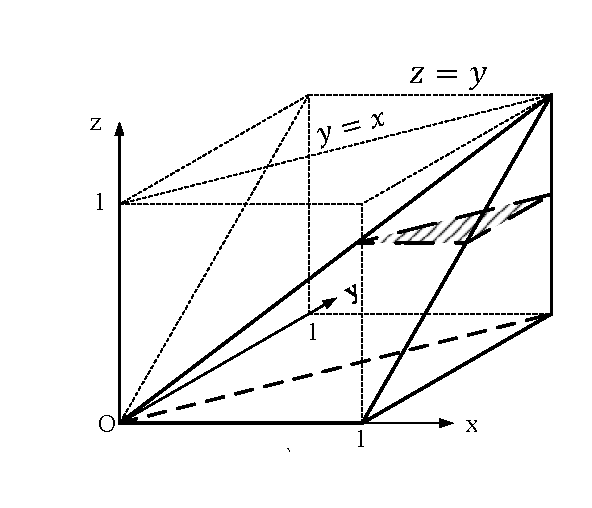
\includegraphics[height=0.4\textheight]{Figures19/Fig12-4-1.pdf}
\end{center}
\caption{习题12.4 1.题图示}
\label{12-4-1}
\end{figure}

解:$I=\Int01{}x\Int0x{}y\Int0y{\frac{\sin z}{(1-z)^2}}z=\Int01{\frac{\sin z}{(1-z)^2}}z\Int z1{}y\Int y1{}x=\Int01{\frac{\sin z}{(1-z)^2}}z\Int z1{(1-y)}y\\
=\Int01{\frac{\sin z}{(1-z)^2}(y-\frac12 y^2)\big|_z^1}z=\Int01{\frac{\sin z}{(1-z)^2}(\frac12-z+\frac12z^2)}z=\frac12\Int01{\frac{\sin z}{(1-z)^2}(1-z)^2}z\\
=\frac12\Int01{\sin z}z=\frac12(-\cos z)\big|_0^1=\frac12(1-\cos1)$.

\item用直角坐标计算三重积分$\varIIInt{\Omega}zxyz$,其中$\Omega$由曲面$x^2+y^2-2z^2=1$,平面$z=1$及$z=2$围成.

\begin{figure}[H]
\begin{center}
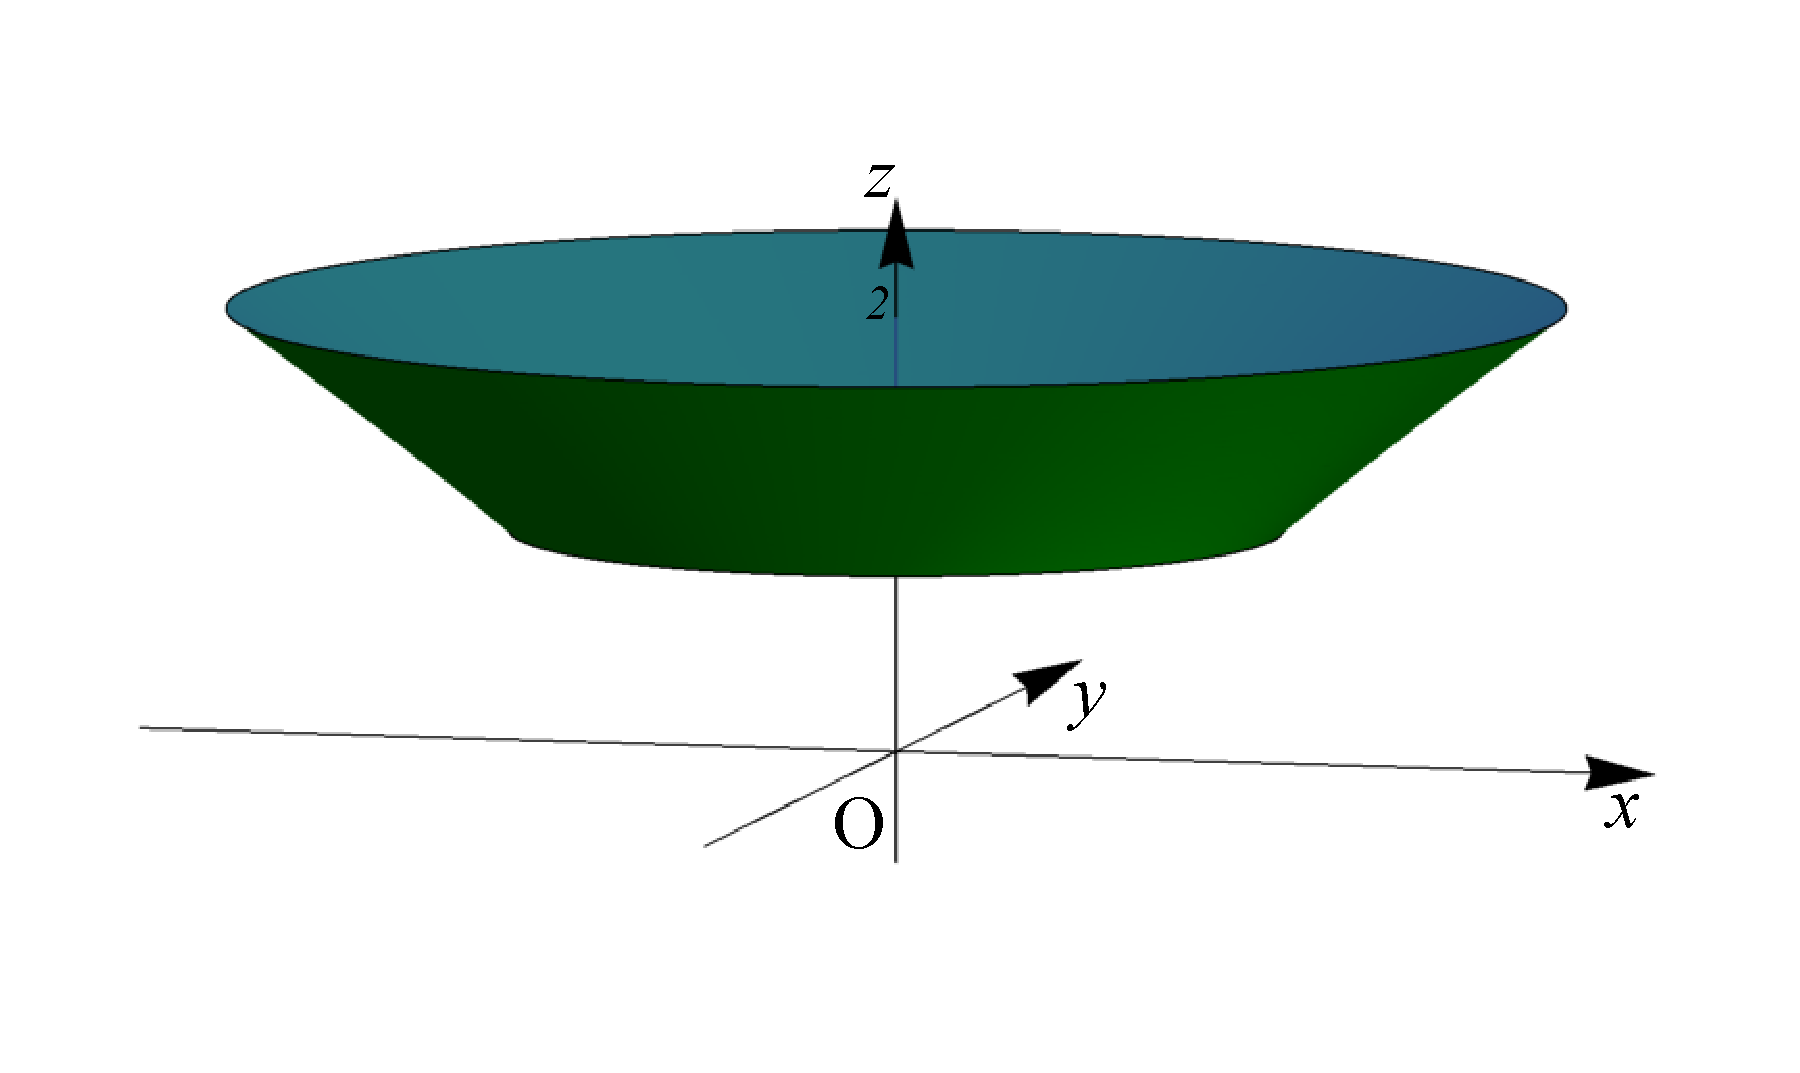
\includegraphics[height=0.4\textheight]{Figures19/Fig12-4-2.pdf}
\end{center}
\caption{习题12.4 2.题图示}
\label{12-4-2}
\end{figure}

解:$\varIIInt{\Omega}zxyz=\Int12zz\varIInt{\Omega_z}{}xy=\Int12{z\pi(1+2z^2)}z=\pi(\frac12z^2+\frac12z^4)\big|_1^2=9\pi$.

\item用柱面坐标计算三重积分$\varIIInt\Omega{\sqrt{y^2+z^2}}xyz$,其中$\Omega$为$y^2+z^2\leqslant x^2,1\leqslant x\leqslant2$.

\begin{figure}[H]
\begin{center}
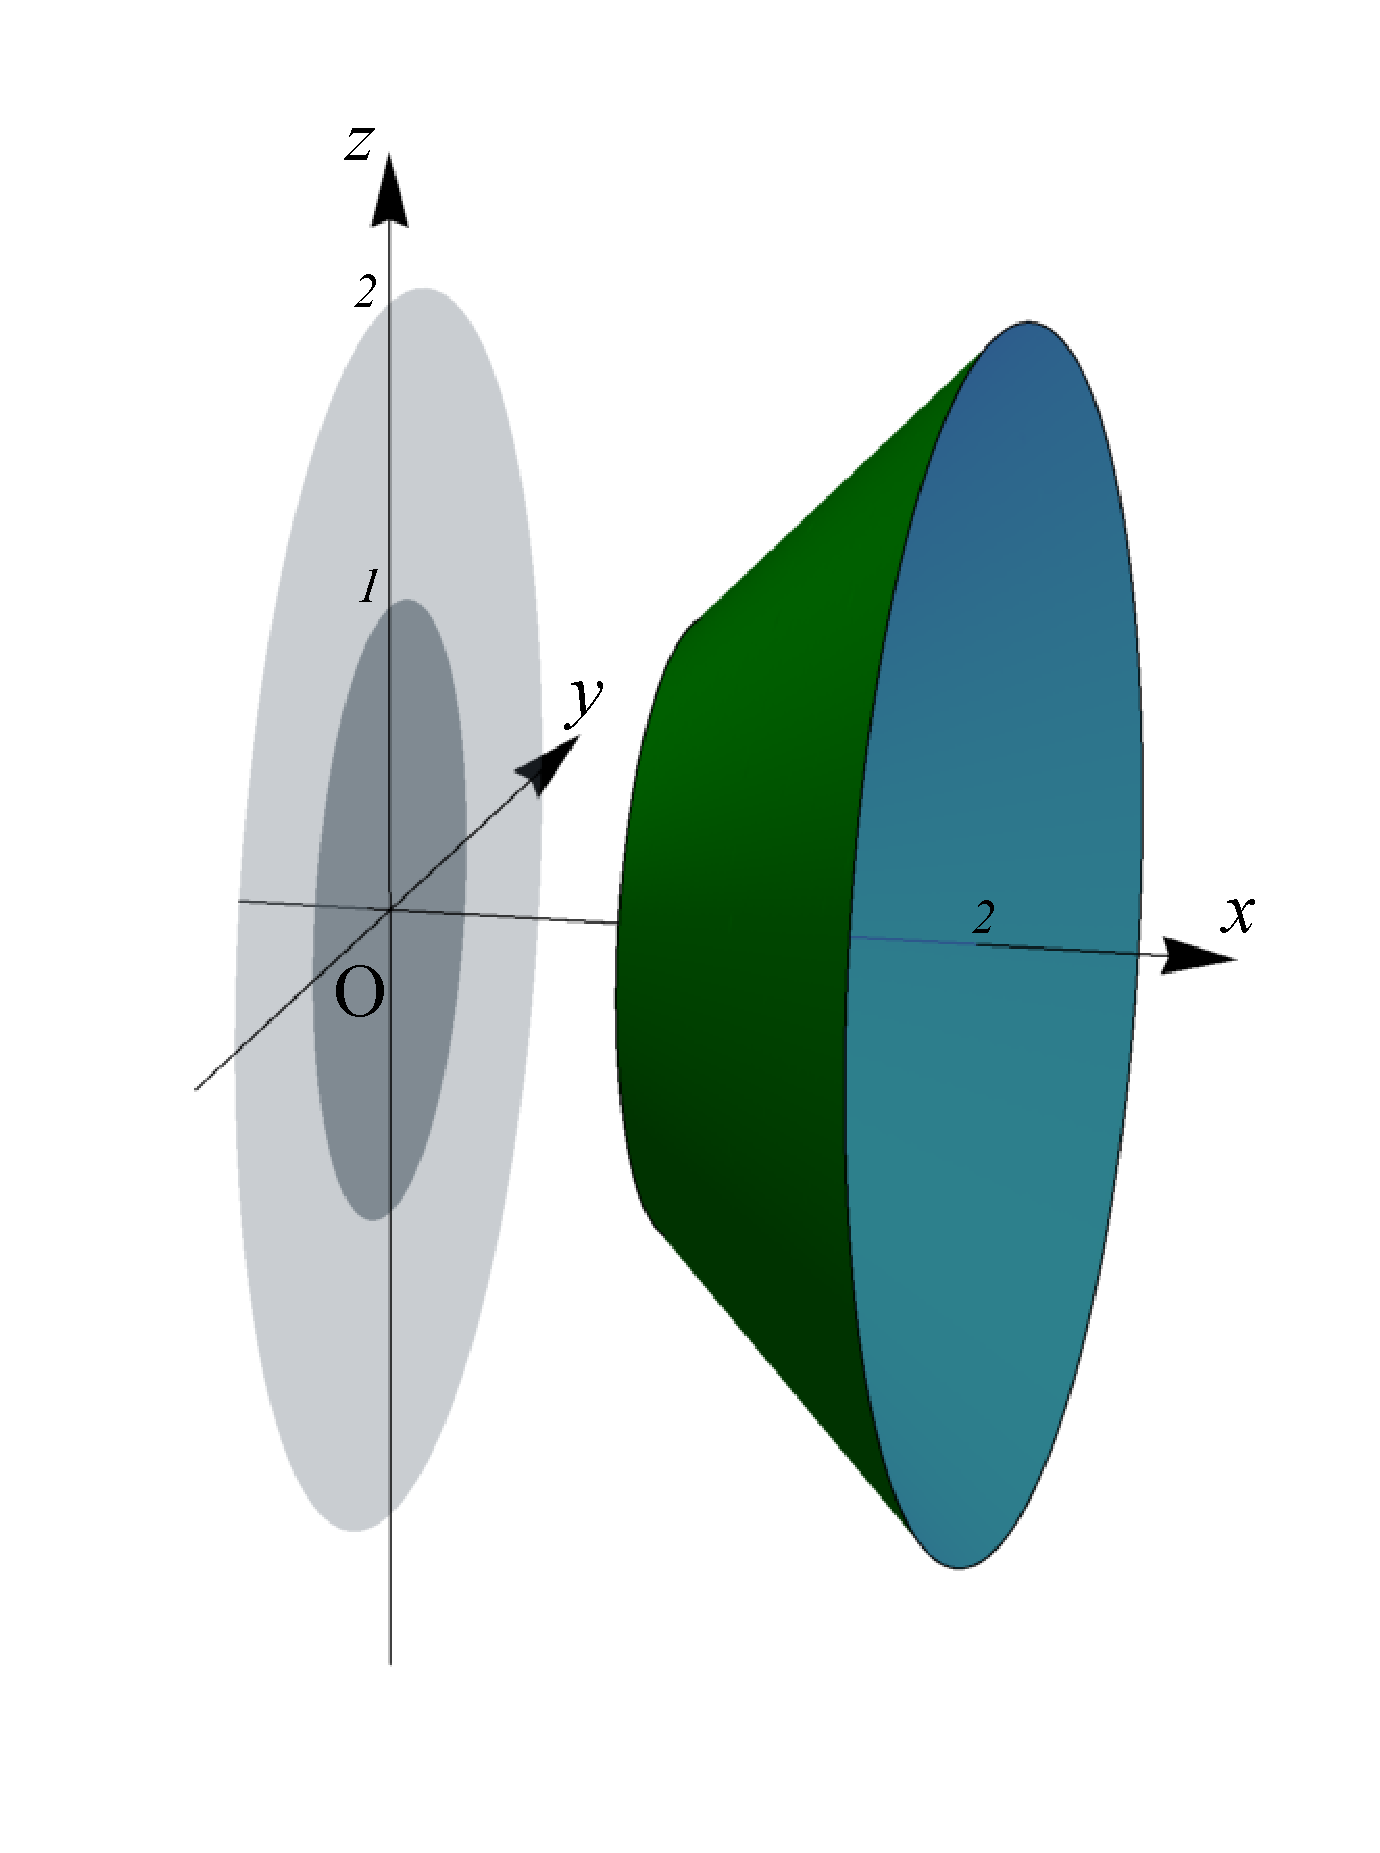
\includegraphics[height=0.4\textheight]{Figures19/Fig12-4-3.pdf}
\end{center}
\caption{习题12.4 3.题图示}
\label{12-4-3}
\end{figure}

解:$\because\Omega=\Set{(x,y)}{y^2+z^2\leqslant x^2,1\leqslant x\leqslant2}=\Set{(x,y)}{y^2+z^2\leqslant1,1\leqslant x\leqslant2}\cup\\
\Set{(x,y)}{1\leqslant y^2+z^2\leqslant x^2,1\leqslant x\leqslant2}=\Omega_1\cup\Omega_2$,

$\therefore\varIIInt\Omega{\sqrt{y^2+z^2}}xyz=\varIIInt{\Omega_1}{\sqrt{y^2+z^2}}xyz+\varIIInt{\Omega_2}{\sqrt{y^2+z^2}}xyz\\
=\Int0{2\pi}{}\theta\Int01{}r\Int12{r\cdot r}x+\Int0{2\pi}{}\theta\Int12{}r\Int r2{r\cdot r}x=2\pi\Int01{r^2}r+2\pi\Int12{r^2(2-r)}r\\
=2\pi\frac13r^3\big|_0^1+2\pi(\frac23r^3-\frac14r^4)\big|_1^2=\frac52\pi$.

\item(1)用球面坐标计算三重积分$\varIIInt\Omega zxyz$,其中$\Omega$由曲面$z=\sqrt{a^2-x^2-y^2}$及$z=\sqrt{x^2+y^2}$围成;\\
(2)设$\Omega$是由曲面$z=\sqrt{x^2+y^2}$与$z=\sqrt{1-x^2-y^2}$围成的空间区域,求$\IIInt\Omega{(x+z)}V$.

\begin{figure}[H]
\begin{center}
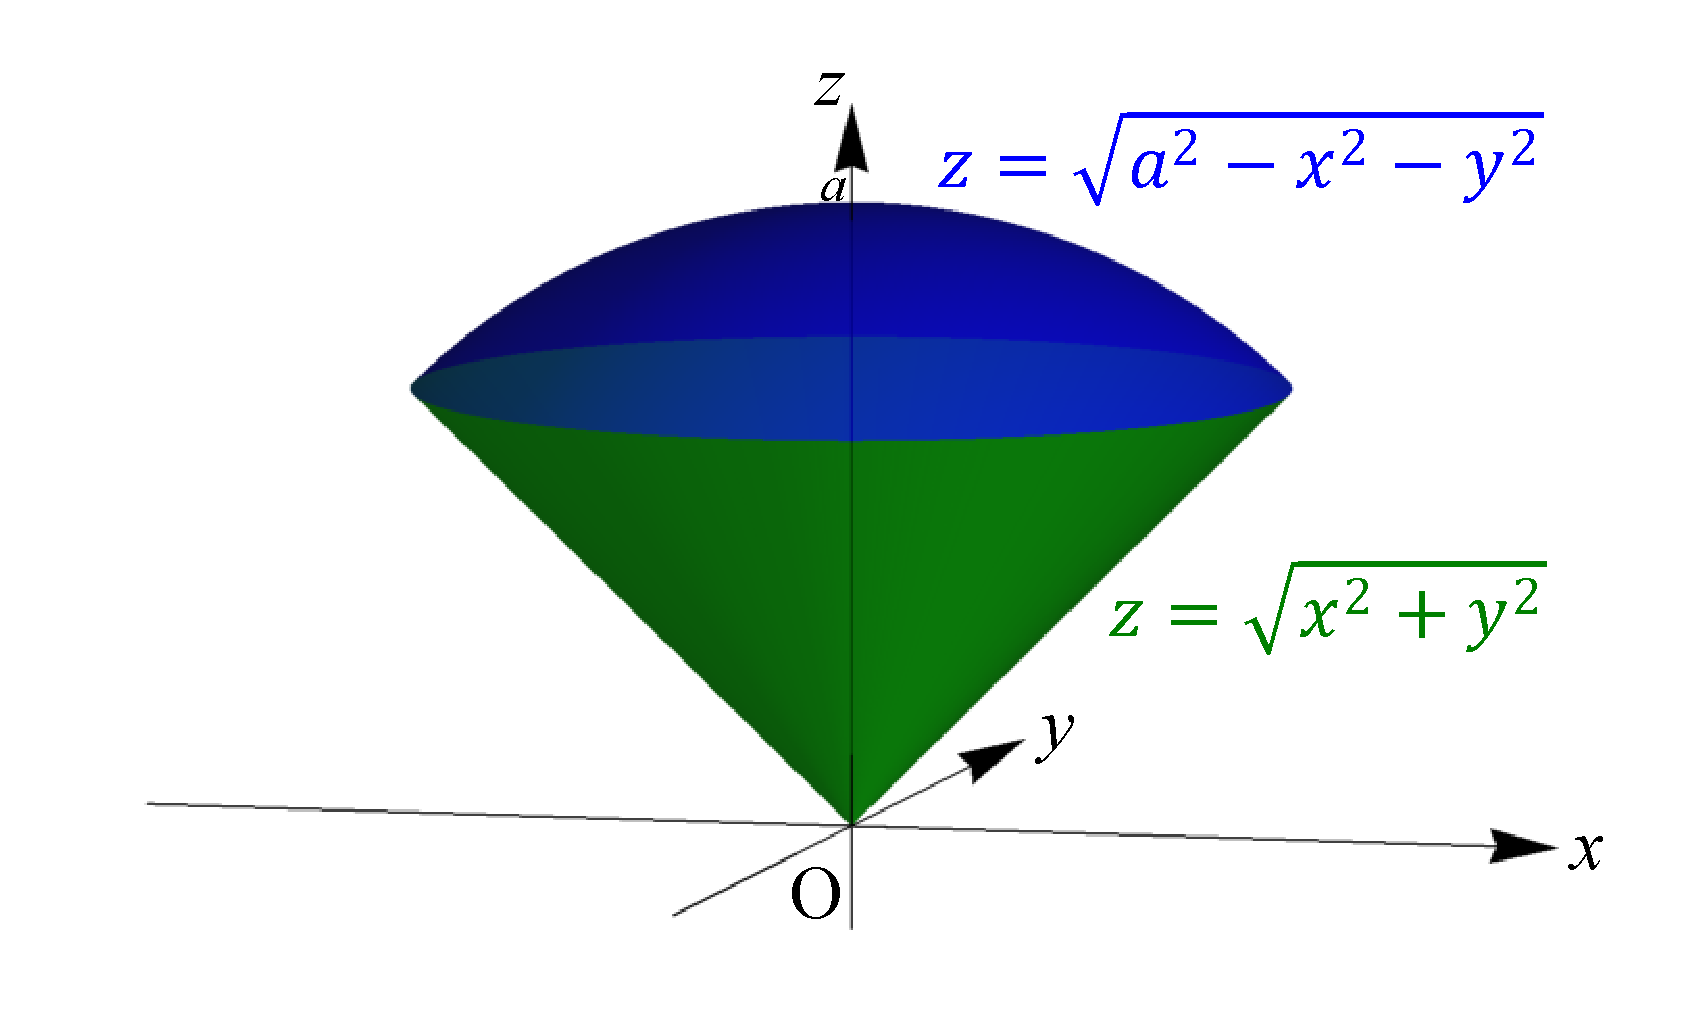
\includegraphics[height=0.4\textheight]{Figures19/Fig12-4-4-1.pdf}
\end{center}
\caption{习题12.4 4.(1)题图示}
\label{12-4-4-1}
\end{figure}

解:(1)$\because$曲面$z=\sqrt{a^2-x^2-y^2}$和$z=\sqrt{x^2+y^2}$的交线所在的投影柱面为$x^2+y^2=\frac{a^2}2$,

$\therefore$交线对应的极角正弦$\sin\varphi_0=\frac{\frac a{\sqrt2}}{a}=\frac1{\sqrt2}$,

$\therefore\varphi_0=\frac\pi4$,

$\therefore\varIIInt\Omega zxyz=\Int0{\frac\pi4}{}\varphi\Int0{2\pi}{}\theta\Int0a{r\cos\varphi r^2\sin\varphi}r=2\pi\Int0{\frac\pi4}{\sin\varphi\cos\varphi}\varphi\Int0a{r^3}r\\
=2\pi\cdot\frac12\sin^2\varphi\big|_0^{\frac\pi4}\cdot\frac14r^4\big|_0^a=\frac\pi8a^4$.

(2)由对称性可知$\IIInt\Omega{x}V=0$,

$\therefore\IIInt\Omega{(x+z)}V=\varIIInt\Omega{z}xyz=\frac\pi8$.

\item设$\Omega$是由曲线$\begin{cases}
x=0,\\
y^2=2z,
\end{cases}$绕$z$轴旋转一周而成的曲面与平面$z=4$围成的空间区域,求$\IIInt\Omega{(x^2+y^2+z)}V$.

\begin{figure}[H]
\begin{center}
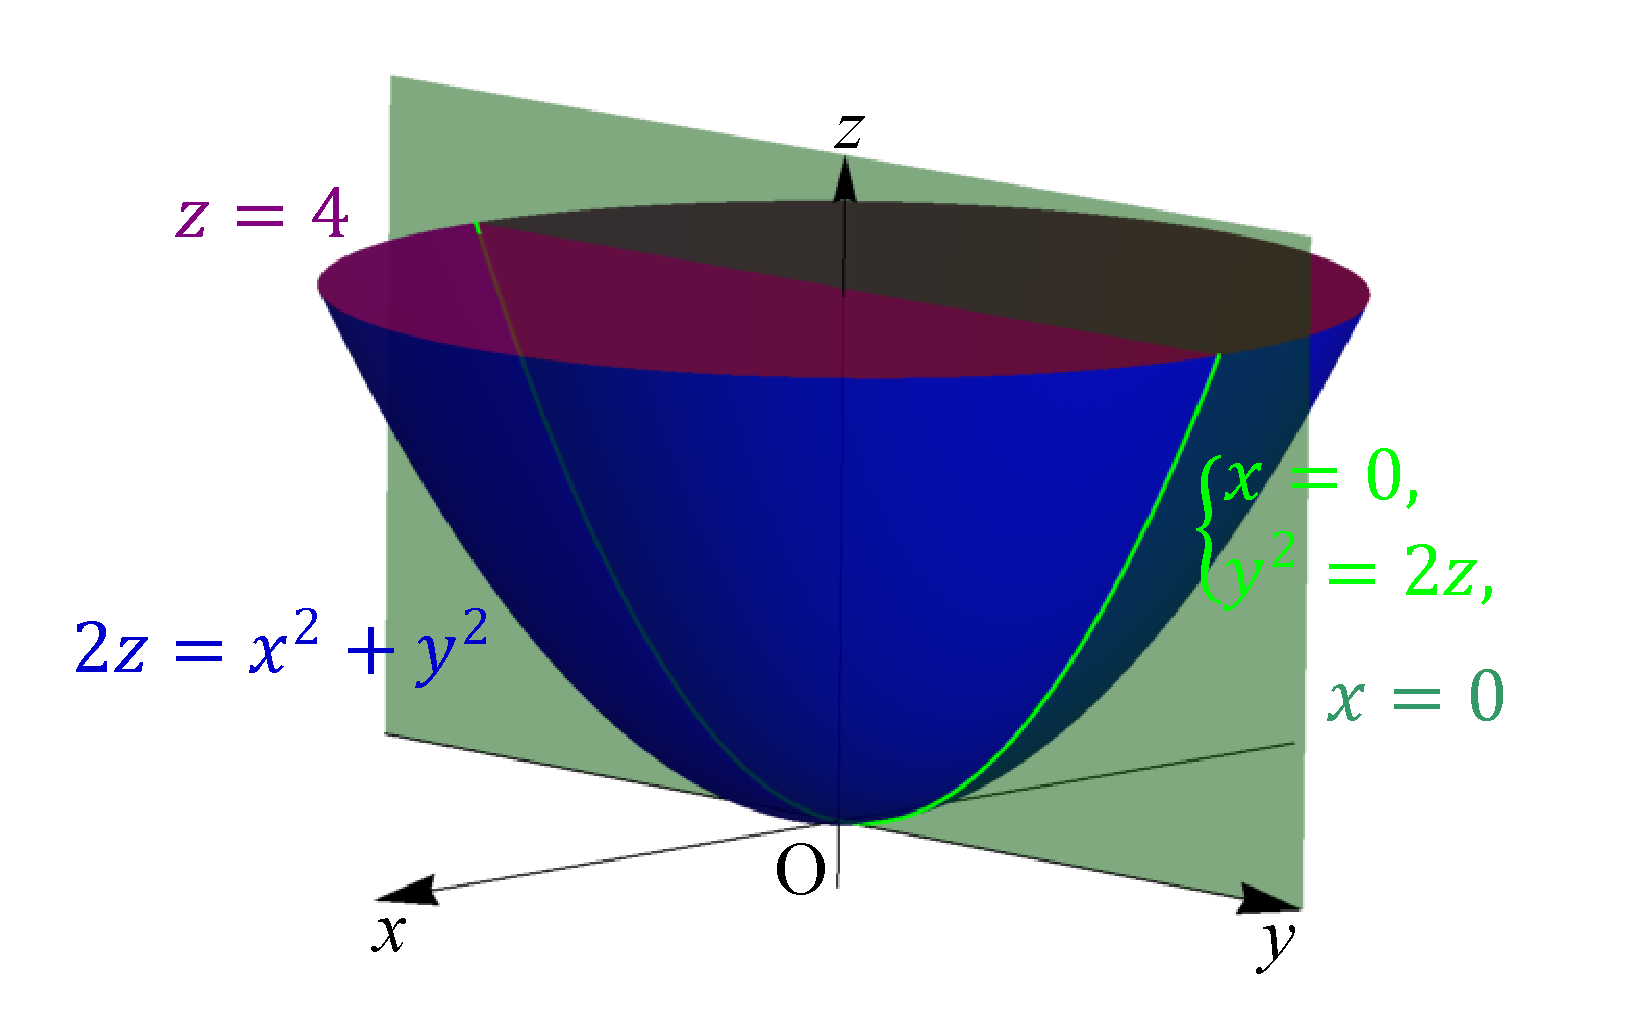
\includegraphics[height=0.4\textheight]{Figures19/Fig12-4-5.pdf}
\end{center}
\caption{习题12.4 5.题图示}
\label{12-4-5}
\end{figure}

解:$\Omega=\Set{(x,y)}{x^2+y^2\leqslant2z,0\leqslant z\leqslant4}$,

$\therefore\IIInt\Omega{(x^2+y^2+z)}V=\Int0{2\pi}{}\theta\Int0{2\sqrt2}{}r\Int{\frac12r^2}4{(r^2+z)r}z=2\pi\Int0{2\sqrt2}{(r^3z+\frac12rz^2)_{\frac12r^2}^4}r\\
=2\pi\Int0{2\sqrt2}{(4r^3+8r-\frac12r^5-\frac18r^5)}r=2\pi(r^4+4r^2-\frac58\cdot\frac16r^6)\big|_0^{2\sqrt2}=\frac{256}3\pi$.

\item在直角坐标、柱坐标和球坐标系下将积分$I=\IIInt\Omega{z^2}V$化为累次积分,并选择其中一种坐标计算,其中$\Omega=\Set{(x,y,z)}{x^2+y^2+z^2\leqslant R^2,x^2+y^2+(z-R)^2\leqslant R^2}$.

\begin{figure}[H]
\begin{center}
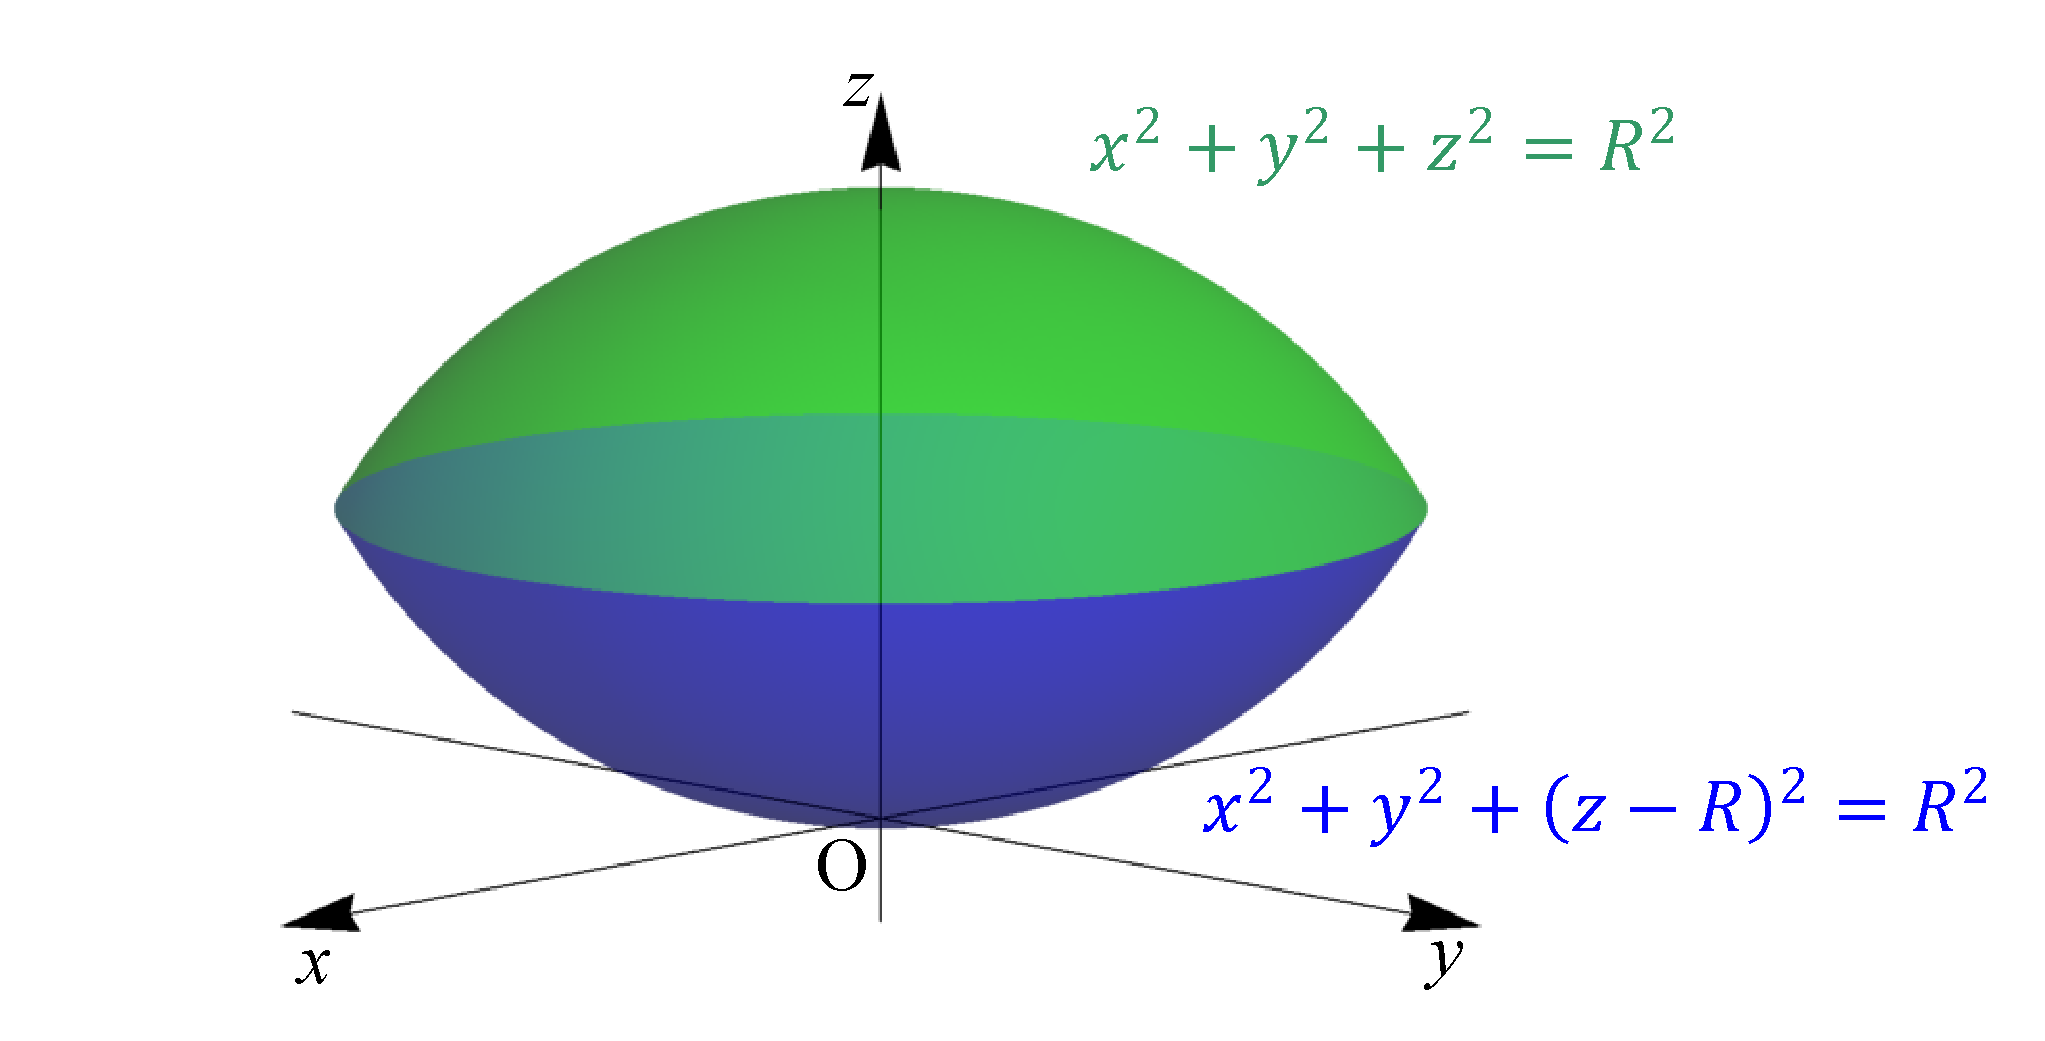
\includegraphics[height=0.4\textheight]{Figures19/Fig12-4-6-1.pdf}
\end{center}
\caption{习题12.4 6.题积分域}
\label{12-4-6}
\end{figure}

解:由$\begin{cases}
x^2+y^2+z^2=R^2,\\
x^2+y^2+(z-R)^2=R^2,
\end{cases}$得交线$\begin{cases}
z=\frac R2,\\
x^2+y^2=\frac34R^2,
\end{cases}$\\
交线对应的极角的正弦$\sin\varphi_0=\frac{\sqrt3}2$,则$\varphi_0=\frac\pi3$.

在直角坐标系下:

\begin{figure}[H]
\begin{center}
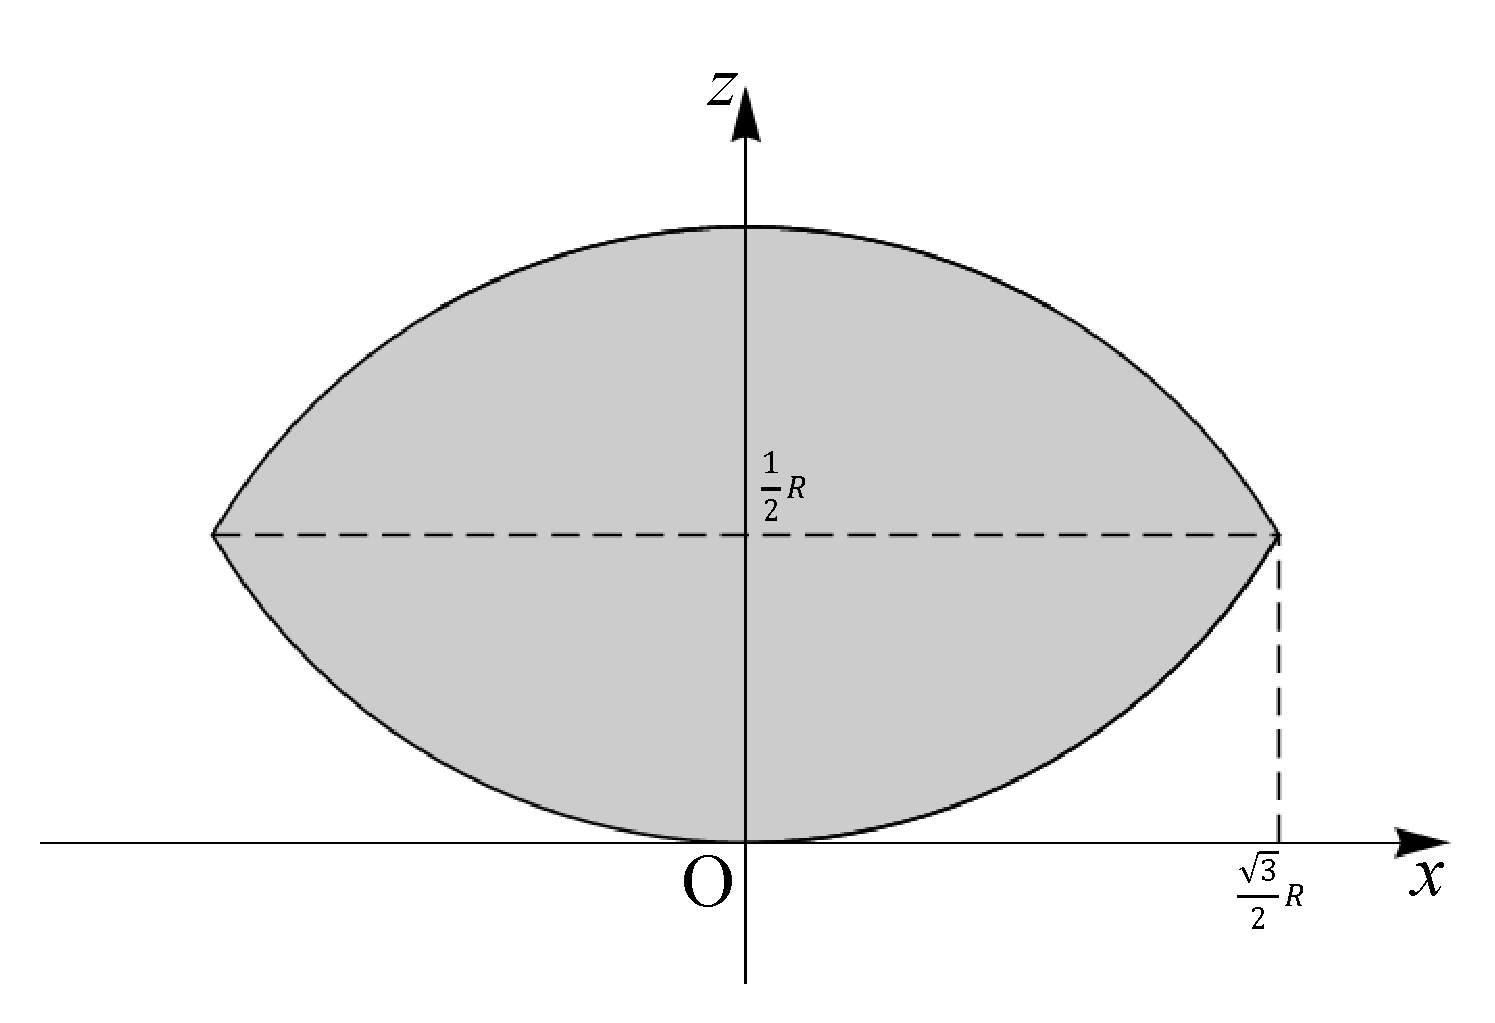
\includegraphics[height=0.4\textheight]{Figures19/Fig12-4-6-2.pdf}
\end{center}
\caption{习题12.4 6.题积分域在$xOz$坐标面上的截面图形(直角坐标系)}
\label{12-4-6-2}
\end{figure}

$I=\IIInt\Omega{z^2}V=\Int0{\frac R2}{z^2}z\varIInt{\Omega_z}{}xy+\Int{\frac R2}R{z^2}z\varIInt{\Omega_z}{}xy\\
=\Int0{\frac R2}{z^2\pi[R^2-(z-R)^2]}z+\Int{\frac R2}R{z^2\pi(R^2-z^2)}z\\
=\pi\Int0{\frac R2}{(2Rz^3-z^4)}z+\pi\Int{\frac R2}R{(R^2z^2-z^4)}z\\
=\pi(\frac12Rz^4-\frac15z^5)\big|_0^{\frac R2}+\pi(\frac13R^2z^3-\frac15z^5)\big|_{\frac R2}^R=\frac{59}{480}\pi R^5$.

或者:


$I=\IIInt\Omega{z^2}V=\Int{-\frac{\sqrt3}2R}{\frac{\sqrt3}2R}{}x\Int{-\sqrt{\frac34R^2-x^2}}{\sqrt{\frac34R^2-x^2}}{}y\Int{R-\sqrt{R^2-x^2-y^2}}{\sqrt{R^2-x^2-y^2}}{z^2}z$.

在柱坐标系下:

$I=\IIInt\Omega{z^2}V=\Int0{2\pi}{}\theta\Int0{\frac{\sqrt3}2R}{}r\Int{R-\sqrt{R^2-r^2}}{\sqrt{R^2-r^2}}{z^2r}z$.

在球坐标系下:
 
\begin{figure}[H]
\begin{center}
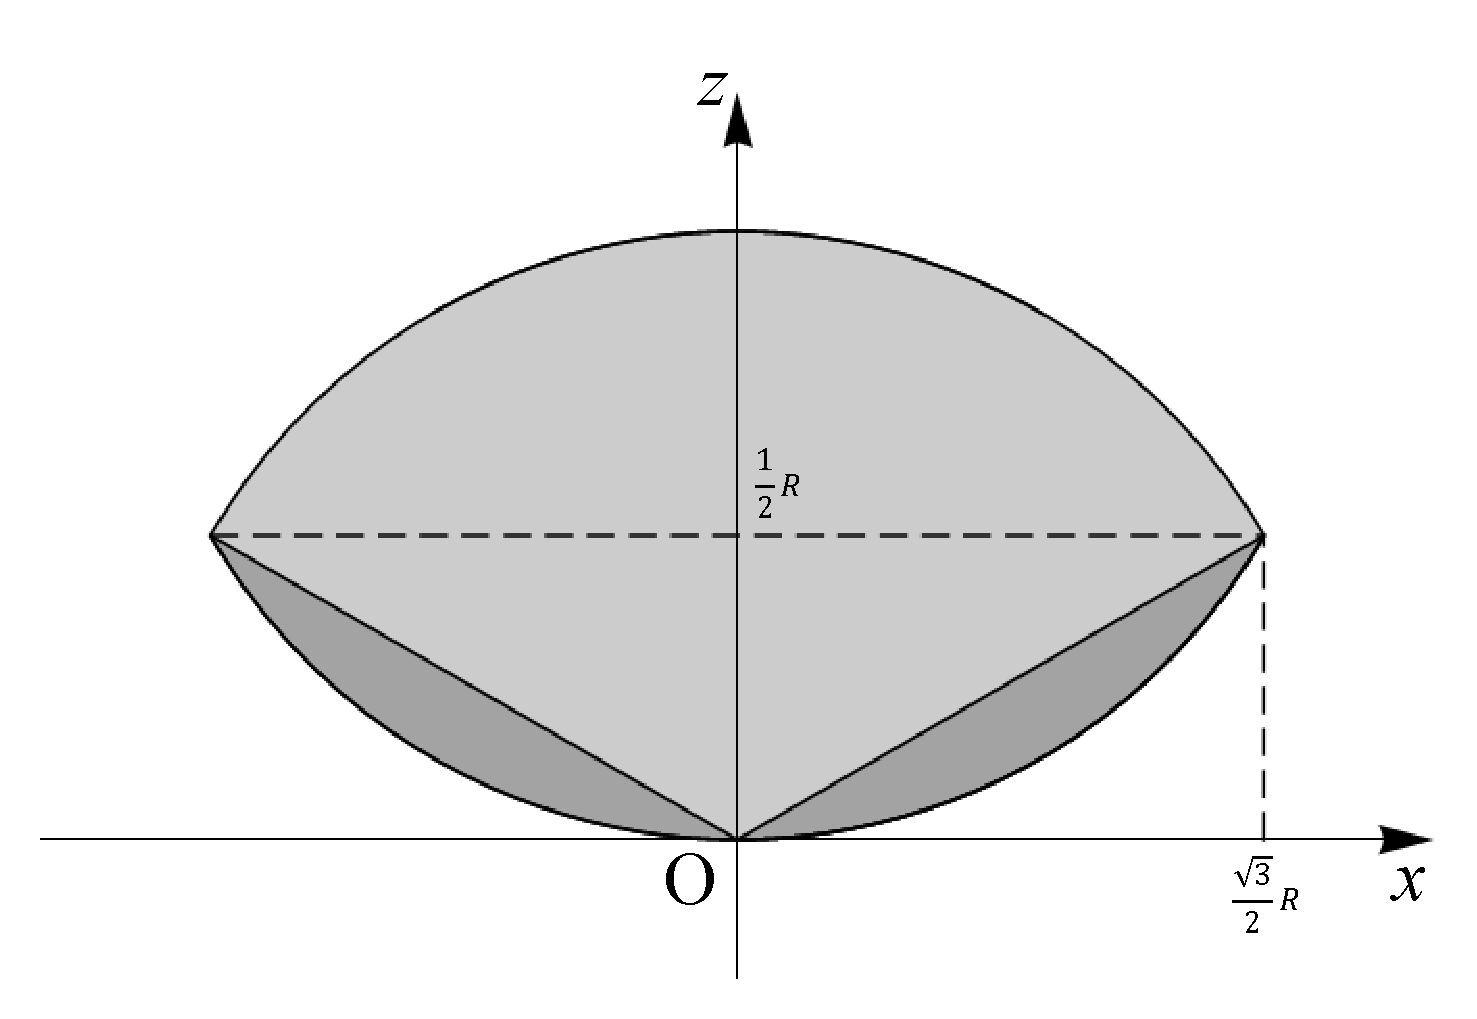
\includegraphics[height=0.4\textheight]{Figures19/Fig12-4-6-3.pdf}
\end{center}
\caption{习题12.4 6.题积分域在$xOz$坐标面上的截面图形(球坐标系)}
\label{12-4-6-3}
\end{figure}

$I=\IIInt\Omega{z^2}V=\Int0{\frac\pi3}{}\varphi\Int0{2\pi}{}\theta\Int0R{r^2\cos^2\varphi r^2\sin\varphi}r+\Int{\frac\pi3}{\frac\pi2}{}\varphi\Int0{2\pi}{}\theta\Int0{2R\cos\varphi}{r^2\cos^2\varphi r^2\sin\varphi}r\\
=2\pi\Int0{\frac\pi3}{\cos^2\varphi\sin\varphi}\varphi\Int0R{r^4}r+2\pi\Int{\frac\pi3}{\frac\pi2}{}\varphi\Int0{2R\cos\varphi}{r^4\cos^2\varphi\sin\varphi}r\\
=2\pi(-\frac13\cos^3\varphi)\big|_0^{\frac\pi3}\frac15r^5\big|_0^R+2\pi\Int{\frac\pi3}{\frac\pi2}{\cos^2\varphi\sin\varphi\frac15r^5\big|_0^{2R\cos\varphi}}\varphi\\
=2\pi(\frac13-\frac13\frac18)\frac15R^5+2\pi\Int{\frac\pi3}{\frac\pi2}{\frac{32}5R^5\cos^7\varphi\sin\varphi}\varphi=2\pi\frac13\cdot\frac78\cdot\frac15-\frac{64\pi}5R^5\frac18\cos^8\varphi\big|_{\frac\pi3}^{\frac\pi2}\\
=\frac{7\pi}{3\times4\times5}-\frac{8\pi}5R^5(0-\frac1{2^8})=\frac{59}{480}\pi R^5$.

\item$\varIIInt\Omega{|z-\sqrt{x^2+y^2}|}xyz$,其中$\Omega$由平面$z=0,z=1$及曲面$x^2+y^2=2$围成.

\begin{figure}[H]
\begin{center}
\subfloat[积分域]{\label{12-4-7-1}
{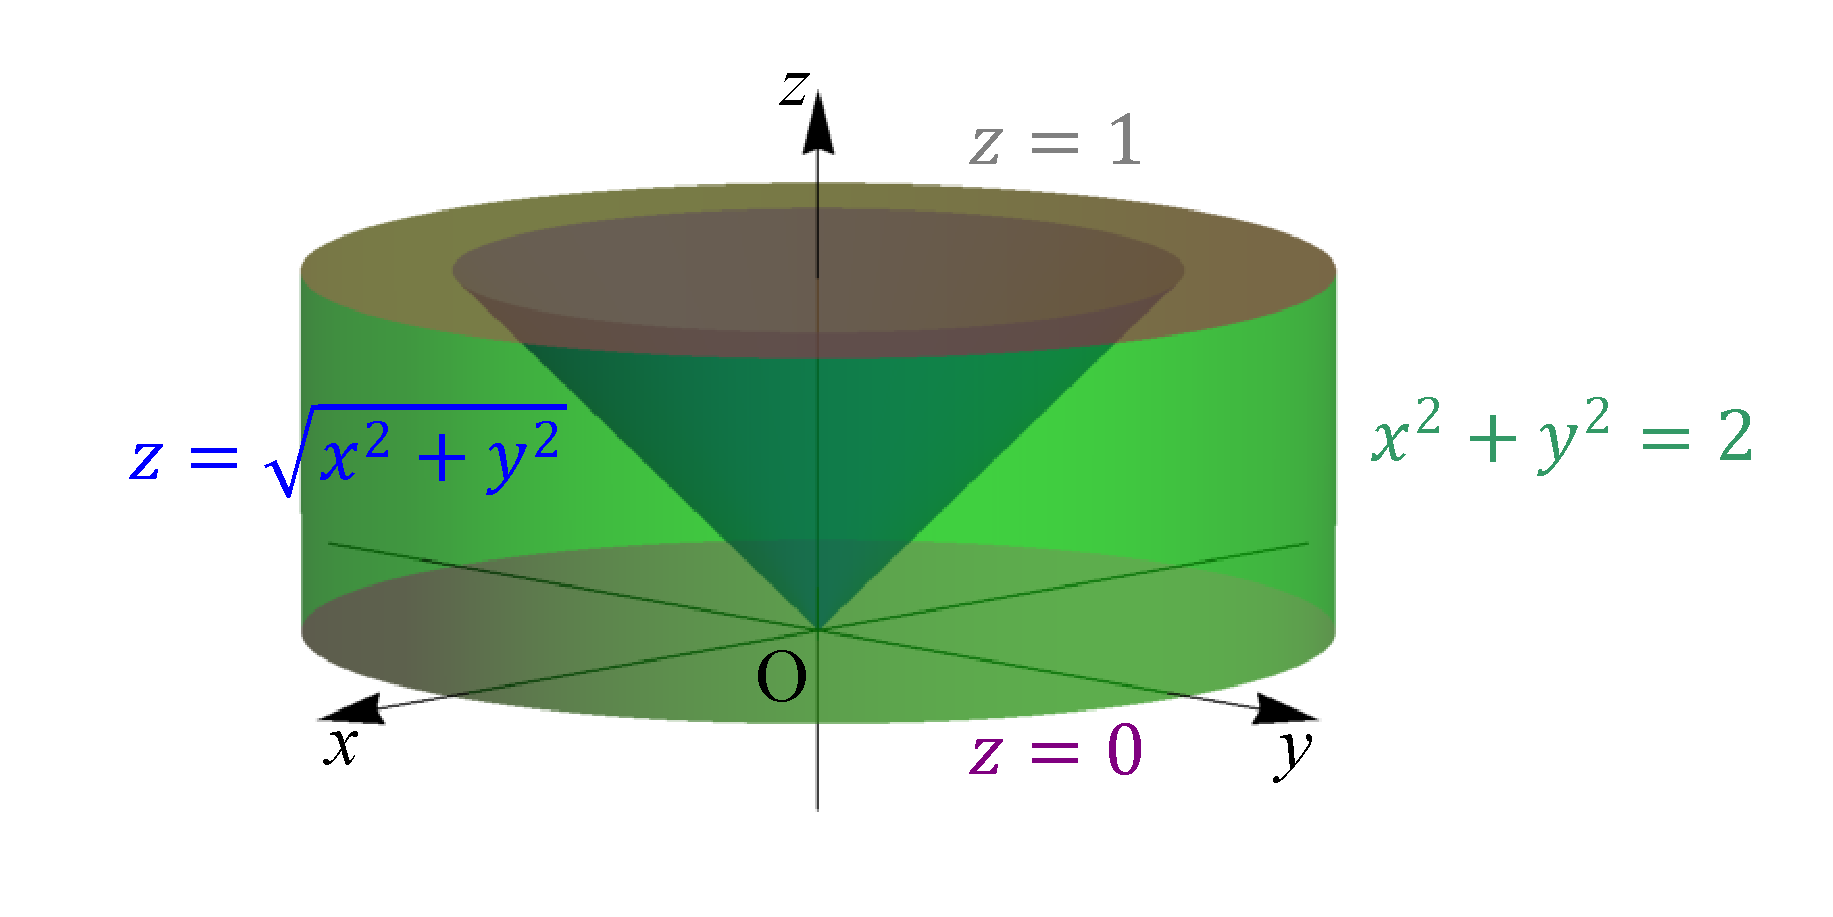
\includegraphics[height=0.3\textheight]{Figures19/Fig12-4-7-1.pdf} }}\\
\subfloat[积分域在$xOz$坐标面上的截面]{\label{12-4-7-2}
{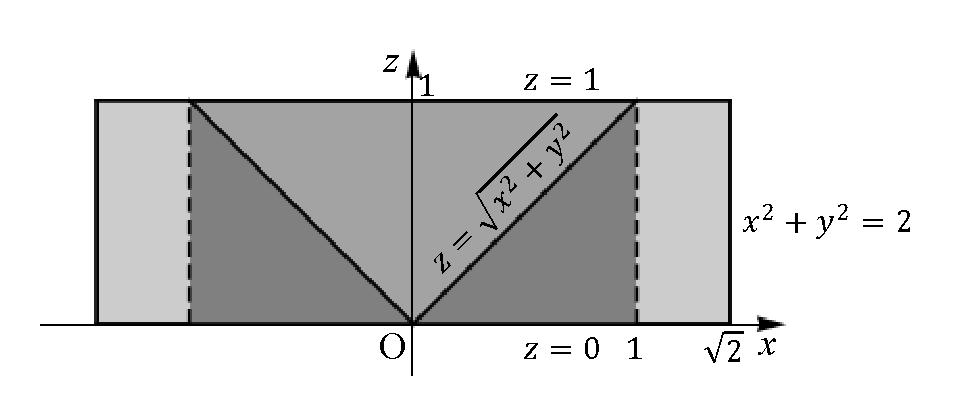
\includegraphics[height=0.3\textheight]{Figures19/Fig12-4-7-2.pdf} }}
\end{center}
\caption{习题12.4 7.题图示}
\label{12-4-7}
\end{figure}

解:$\varIIInt\Omega{|z-\sqrt{x^2+y^2}|}xyz=\Int0{2\pi}{}\theta\Int1{\sqrt2}{}r\Int01{(r-z)r}z+\Int0{2\pi}{}\theta\Int01{}r\Int0{r}{(r-z)r}z+\Int0{2\pi}{}\theta\Int01{}r\Int r1{(z-r)r}z\\
=2\pi\Int1{\sqrt2}{(r^2z-\frac12rz^2)\big|_0^1}r+2\pi\Int01{(r^2z-\frac12rz^2)\big|_0^r}r+2\pi\Int01{(\frac12rz^2-r^2z)\big|_r^1}r\\
=2\pi\Int1{\sqrt2}{(r^2-\frac12r)}r+2\pi\Int01{\frac12r^3}r+2\pi\Int01{(\frac12r-r^2+\frac12r^3)}r\\
=2\pi(\frac13r^3-\frac14r^2)\big|_1^{\sqrt2}+2\pi\frac18r^4\big|_0^1+2\pi(\frac14r^2-\frac13r^3+\frac18r^4)\big|_0^1\\
=2\pi(\frac13\cdot2\sqrt2-\frac14\cdot2-\frac13+\frac14)+2\pi\cdot\frac18+2\pi(\frac14-\frac13+\frac18)=\pi(\frac43\sqrt2-\frac56)$.
%
%注:如图~\ref{12-4-7}所示.
%\begin{figure}[H]
%\begin{center}
%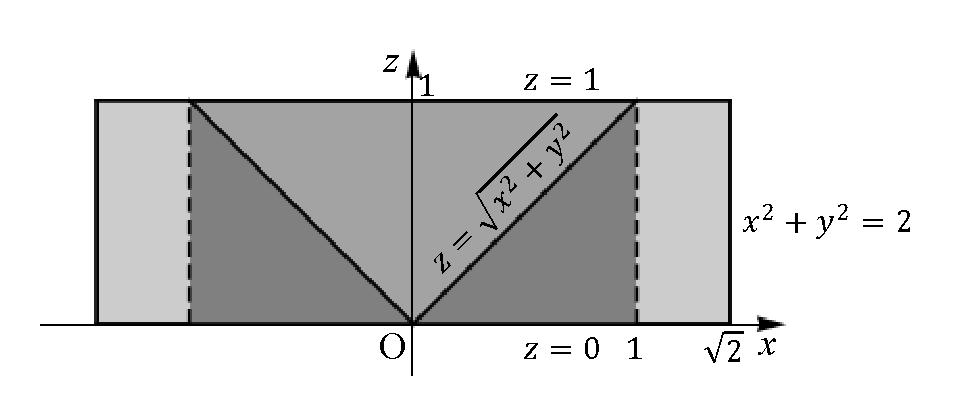
\includegraphics[height=0.2\textheight]{Figures19/Fig12-4-7-2.pdf}
%\end{center}
%\caption{习题12.4 7.题积分域在$xOz$坐标面上的截面}
%\label{12-4-7}
%\end{figure}

\item计算三重积分$\IIInt\Omega{(3x^2+5y^2+7z^2)}V,\Omega:\ x^2+y^2+z^2\leqslant R^2$.

\begin{figure}[H]
\begin{center}
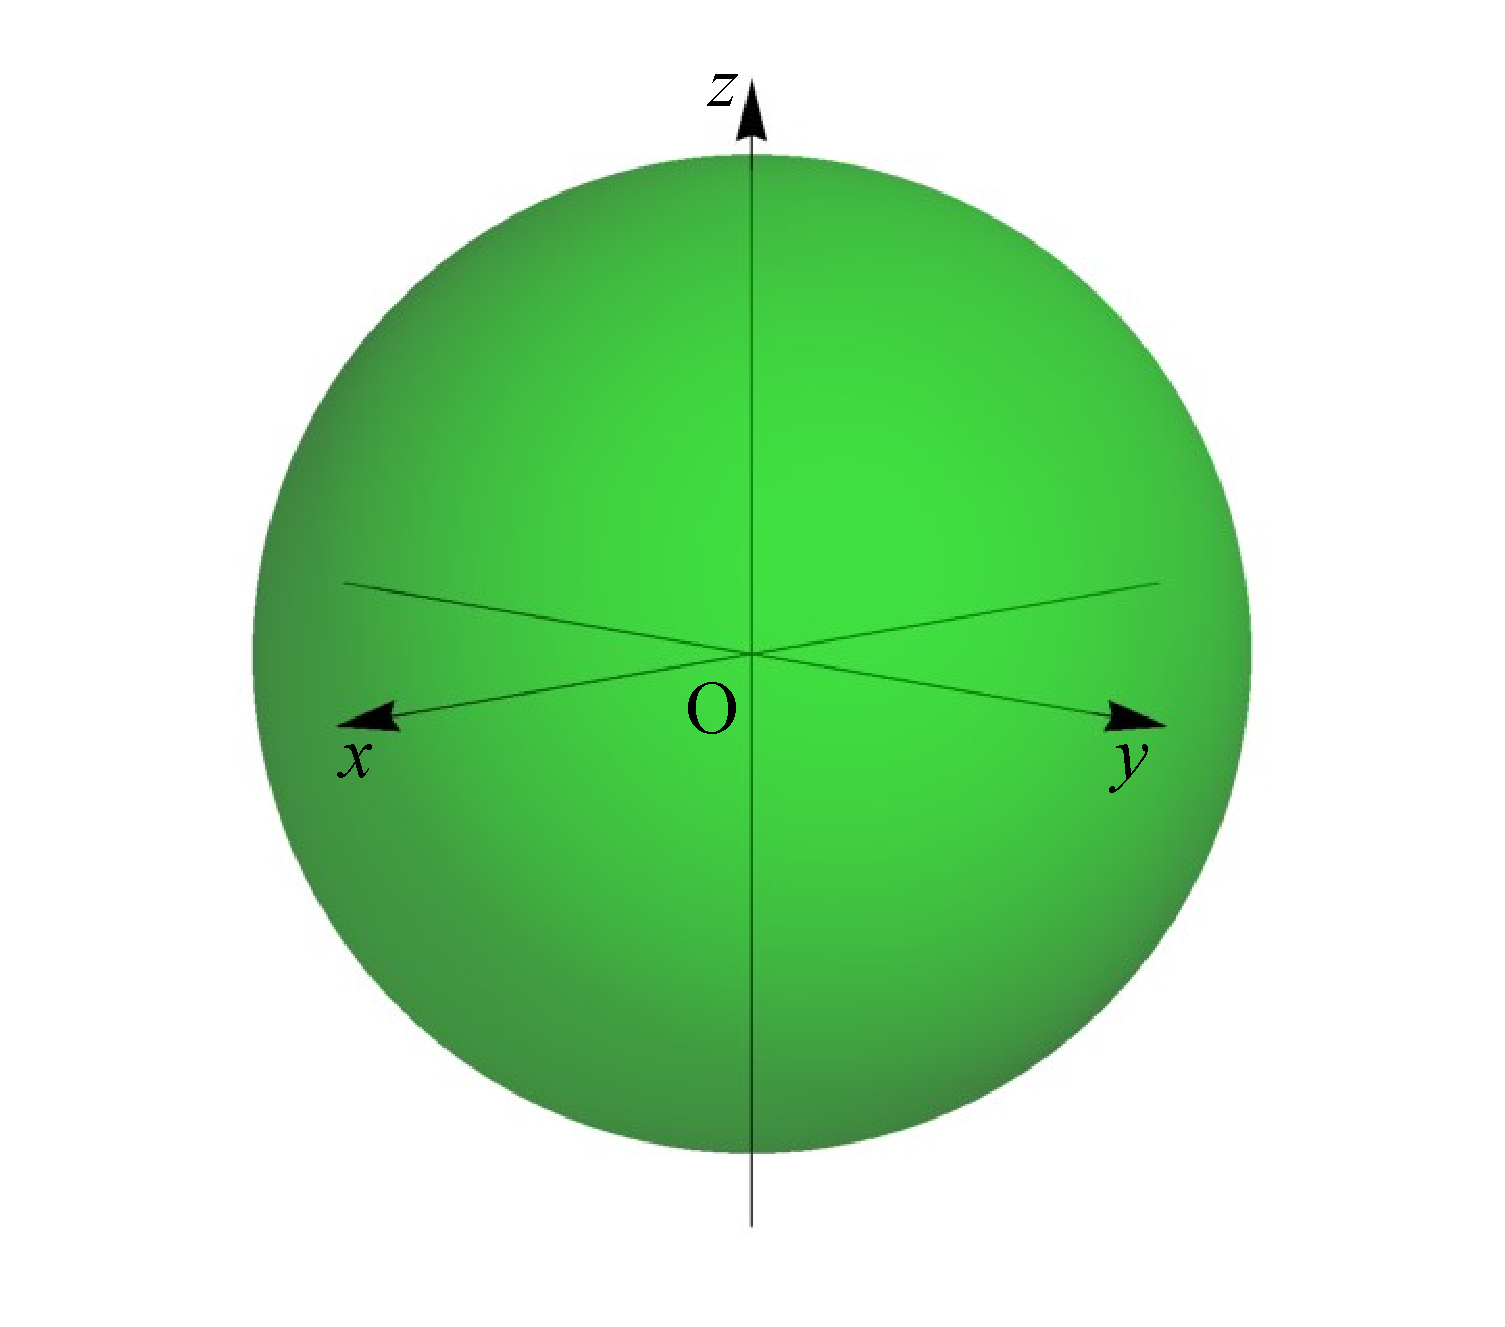
\includegraphics[height=0.4\textheight]{Figures19/Fig12-4-8.pdf}
\end{center}
\caption{习题12.4 8.题积分域}
\label{12-4-8}
\end{figure}

解:$\IIInt\Omega{z^2}V=\Int{-R}R{z^2}z\varIInt{\Omega_z}{}xy=\Int{-R}R{z^2\pi(R^2-z^2)}z=\frac4{15}\pi R^5$,

由对称性可知$\IIInt\Omega{x^2}V=\IIInt\Omega{y^2}V=\IIInt\Omega{z^2}V$,

$\therefore\IIInt\Omega{(3x^2+5y^2+7z^2)}V=(3+5+7)\IIInt\Omega{z^2}V=4\pi R^5$.

\item设$F(t)=\varIIInt\Omega{[z^2+f(x^2+y^2)]}xyz$,其中$f(u)$连续,$\Omega$为$0\leqslant z\leqslant h,x^2+y^2\leqslant t^2$. 试求$\frac{\mathrm dF}{\mathrm dt}\Big|_{t=0}$和$\LIM t0\frac1{t^2}F(t)$.

解:$F(t)=\varIIInt\Omega{[z^2+f(x^2+y^2)]}xyz=\Int0{2\pi}{}\theta\Int0t{}r\Int0h{[z^2+f(r^2)]r}z\\
=2\pi\Int0t{[\frac13rz^3+rf(r)z]\big|_0^h}r=2\pi\Int0t{[\frac13h^3r+hrf(r)]}r$,

$\therefore\frac{\mathrm dF}{\mathrm dt}=2\pi[\frac13h^3t+htf(t)]$,

$\therefore\frac{\mathrm dF}{\mathrm dt}\Big|_{t=0}=0$.

$\therefore\LIM t0\frac1{t^2}F(t)=\LIM t0\frac{\frac{\mathrm dF}{\mathrm dt}}{2t}=\LIM t0\frac{2\pi[\frac13h^3t+htf(t)]}{2t}=\LIM t0\pi[\frac13h^3+hf(t)]=\pi[\frac13h^3+hf(0)]$.

\item设$f(x)$在$[0,1]$上连续,证明:
\[
\Int01{}x\Int x1{}y\Int xy{f(x)f(y)f(z)}z=\frac16(\Int01{f(x)}x)^3.
\]
证明:设$F(u)=\Int0u{f(t)}t$,

$\because f(x)$在$[0,1]$上连续,

$\therefore F'(u)=f(u)$,

方法1:
$\therefore\Int01{}x\Int x1{}y\Int xy{f(x)f(y)f(z)}z=\Int01{f(x)}x\Int x1{f(y)}y\Int xy{f(z)}z\\
=\Int01{f(x)}x\Int x1{f(y)}y[\Int 0y{f(z)}z-\Int0x{f(z)}z]\\
=\Int01{f(x)}x\Int x1{f(y)[F(y)-F(x)]}y\\
=\Int01{f(x)}x\Int x1{[F(y)-F(x)]}{F(y)}\\
=\Int01{f(x)}x\{F(y)[F(y)-F(x)]\big|_x^1-\Int x1{F(y)}{[F(y)-F(x)]}\}\\
=\Int01{f(x)}x\{F(y)[F(y)-F(x)]\big|_x^1-\Int x1{F(y)}{F(y)}\}\\
=\Int01{f(x)}x\{F(1)[F(1)-F(x)]-\frac12[F(y)]^2\big|_x^1\}\\
=\Int01{f(x)}x\{F(1)[F(1)-F(x)]-\frac12[F(1)]^2+\frac12[F(x)]^2\}\\
=\Int01{f(x)}x\{\frac12[F(1)]^2-F(1)F(x)+\frac12[F(x)]^2\}\\
=\Int01{f(x)}x\frac12[F(1)-F(x)]^2=\Int01{\frac12[F(1)-F(x)]^2}{F(x)}\\
=-\frac12\Int01{[F(1)-F(x)]^2}{[F(1)-F(x)]}\\
=-\frac16[F(1)-F(x)]^3\big|_0^1\\
=\frac16[F(1)]^3\\
=\frac16(\Int01{f(x)}x)^3$.

方法2:$\therefore\Int01{}x\Int x1{}y\Int xy{f(x)f(y)f(z)}z\\
=\Int01{f(x)}x\Int x1{f(y)}y\Int xy{f(z)}z\\
=\Int01{f(x)}x\Int x1{f(y)}y[\Int 0y{f(z)}z-\Int0x{f(z)}z]\\
=\Int01{f(x)}x\Int x1{f(y)[F(y)-F(x)]}y\\
=\Int01{f(x)}x\Int x1{[F(y)-F(x)]}{[F(y)-F(x)]}\\
=\Int01{f(x)}x\frac12[F(y)-F(x)]\big|_x^1\\
=\Int01{f(x)}x\frac12[F(1)-F(x)]^2\\
=\Int01{\frac12[F(1)-F(x)]^2}{F(x)}\\
=-\frac12\Int01{[F(1)-F(x)]^2}{[F(1)-F(x)]}\\
=-\frac16[F(1)-F(x)]^3\big|_0^1\\
=\frac16[F(1)]^3\\
=\frac16(\Int01{f(x)}x)^3$.

\item求由$(x^2+y^2)^2=8x^3$围成的区域的面积.

\begin{figure}[H]
\begin{center}
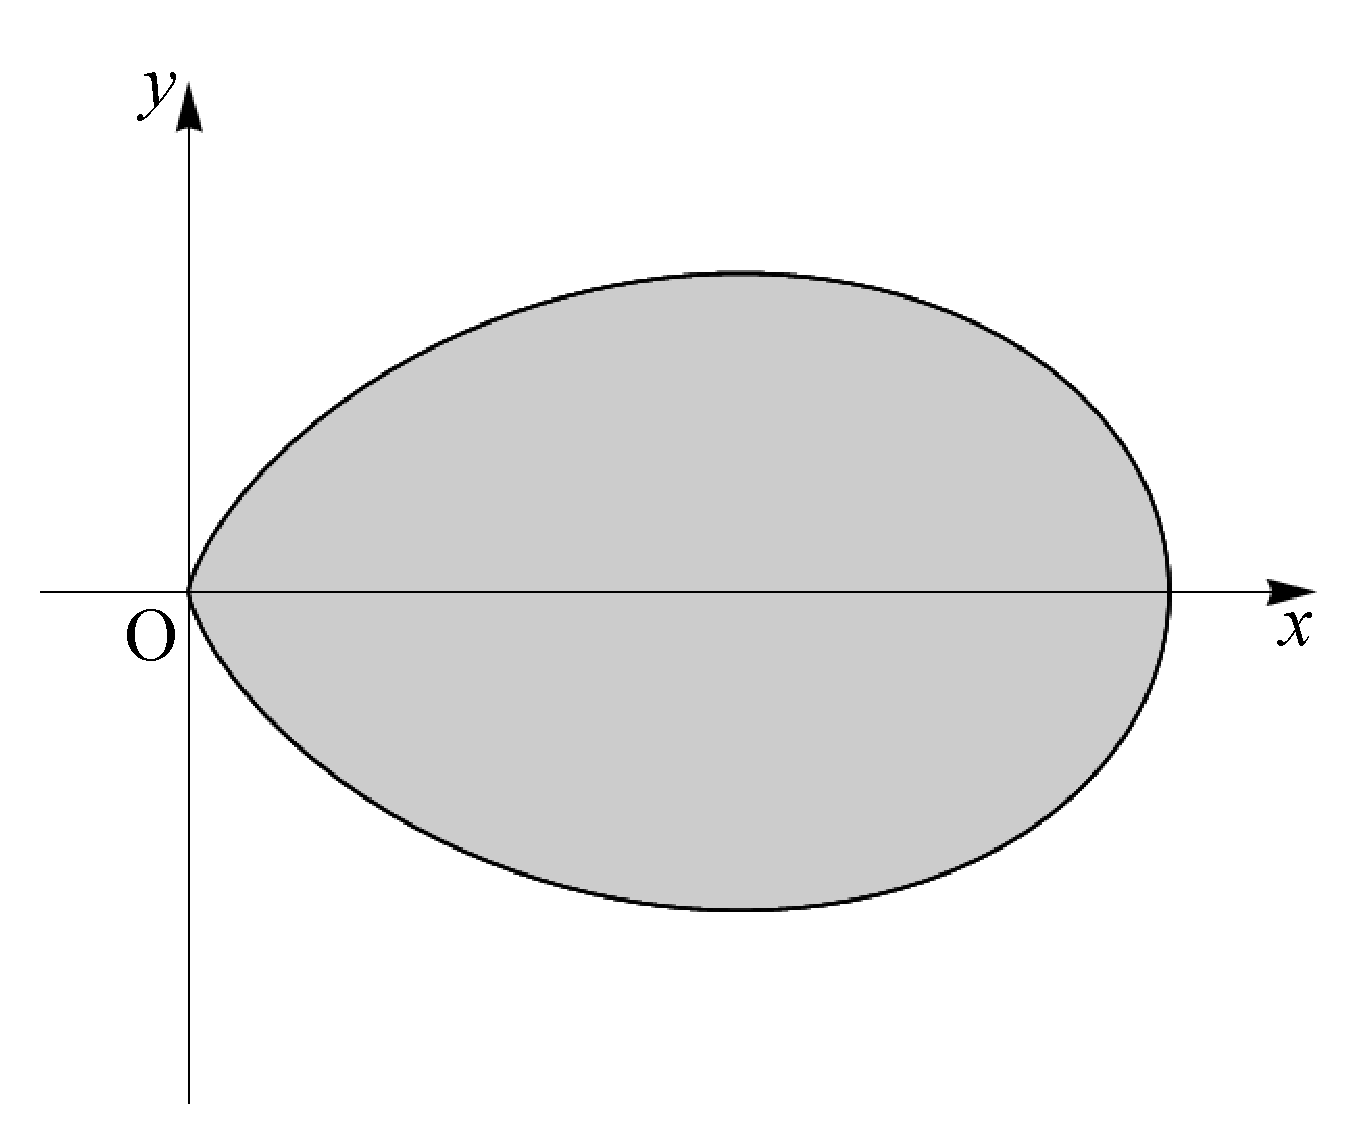
\includegraphics[height=0.4\textheight]{Figures19/Fig12-4-11.pdf}
\end{center}
\caption{习题12.4 11.题积分域}
\label{12-4-11}
\end{figure}

解:$(x^2+y^2)^2=8x^3$在极坐标系中的方程为$r=8\cos^3\theta$,且满足$\cos^3\theta\geqslant0$,即$-\frac\pi2\leqslant\theta\leqslant\frac\pi2$,

$\therefore$该区域用极坐标表示为$D=\Set{(r,\theta)}{0\leqslant r\leqslant8\cos^3\theta,-\frac\pi2\leqslant\theta\leqslant\frac\pi2}$,

$S=\IInt D{}\sigma=\Int{-\frac\pi2}{\frac\pi2}{}\theta\Int0{8\cos^3\theta}rr=\Int{-\frac\pi2}{\frac\pi2}{}\theta\frac12r^2\big|_0^{8\cos^3\theta}=32\Int{-\frac\pi2}{\frac\pi2}{\cos^6\theta}\theta=64\Int0{\frac\pi2}{\cos^6\theta}\theta\\
=64\frac{5\cdot3\cdot1}{6\cdot4\cdot2}\cdot\frac\pi2=10\pi$.

\item求由$r\leqslant a(1+\cos\theta)$与$x^2+y^2\geqslant a^2$确定的平面图形的面积.

\begin{figure}[H]
\begin{center}
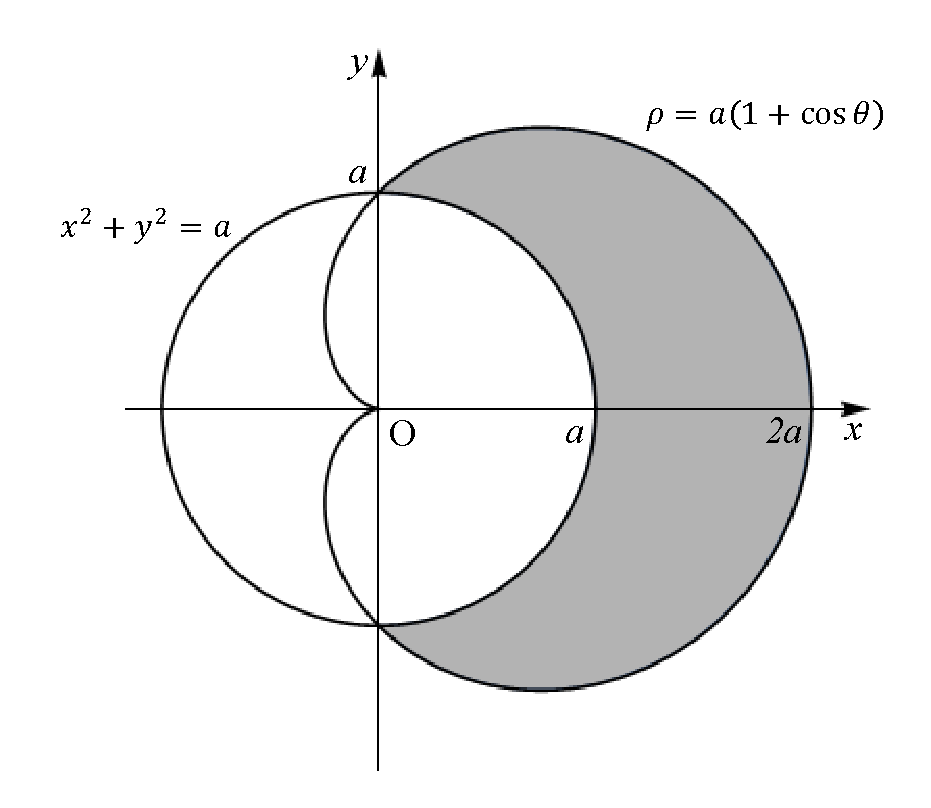
\includegraphics[height=0.4\textheight]{Figures19/Fig12-4-12.pdf}
\end{center}
\caption{习题12.4 12.题图示}
\label{12-4-12}
\end{figure}

解:圆$x^2+y^2=a^2$的极坐标表示为$r=a$,由$\begin{cases}
r=a,\\
r=a(1+\cos\theta),
\end{cases}$得$\theta=\pm\frac\pi2$,

该平面图形可表示为$D=\Set{(r,\theta)}{a\leqslant r\leqslant a(1+\cos\theta),-\frac\pi2\leqslant\theta\leqslant\frac\pi2}$,

$\therefore S=\Int D{}\sigma=\Int{-\frac\pi2}{\frac\pi2}{}\theta\Int a{a(1+\cos\theta)}rr=\Int{-\frac\pi2}{\frac\pi2}{}\theta\frac12r^2\big|_a^{a(1+\cos\theta)}=\frac12a^2\Int{-\frac\pi2}{\frac\pi2}{[(1+\cos\theta)^2-1]}\theta\\
=\frac12a^2\Int{-\frac\pi2}{\frac\pi2}{(2\cos\theta+\cos^2\theta)}\theta=a^2\Int0{\frac\pi2}{(2\cos\theta+\cos^2\theta)}\theta=a^2(2\cdot1+\frac12\cdot\frac\pi2)=(2+\frac\pi4)a^2$.

\item求由抛物面$z=x^2+y^2$与球面$z=\sqrt{6-x^2-y^2}$所围空间图形的体积.

\begin{figure}[H]
\begin{center}
\subfloat[积分域]{\label{12-4-13-1}
{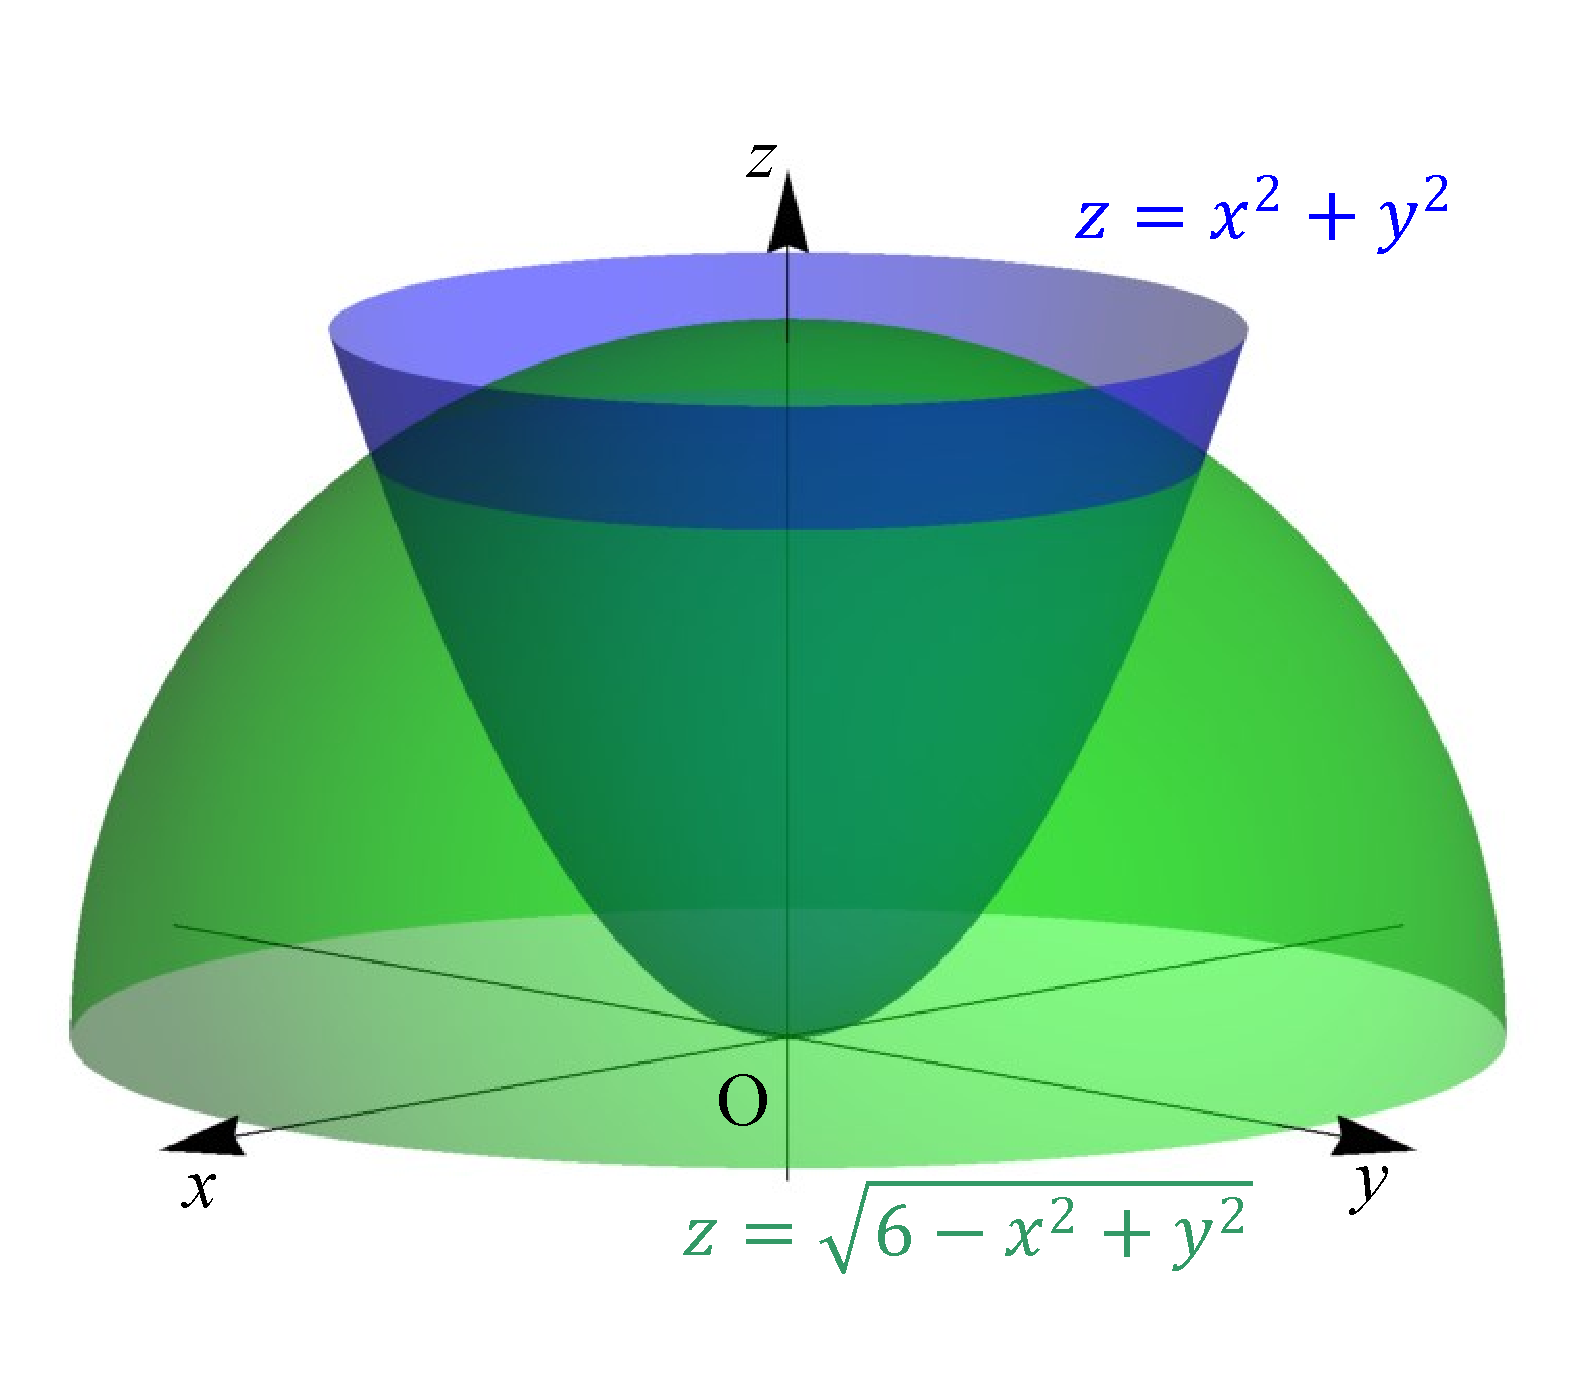
\includegraphics[height=0.4\textheight]{Figures19/Fig12-4-13-2.pdf} }}\\
\subfloat[积分域在$xOz$坐标面上的截面]{\label{12-4-13-2}
{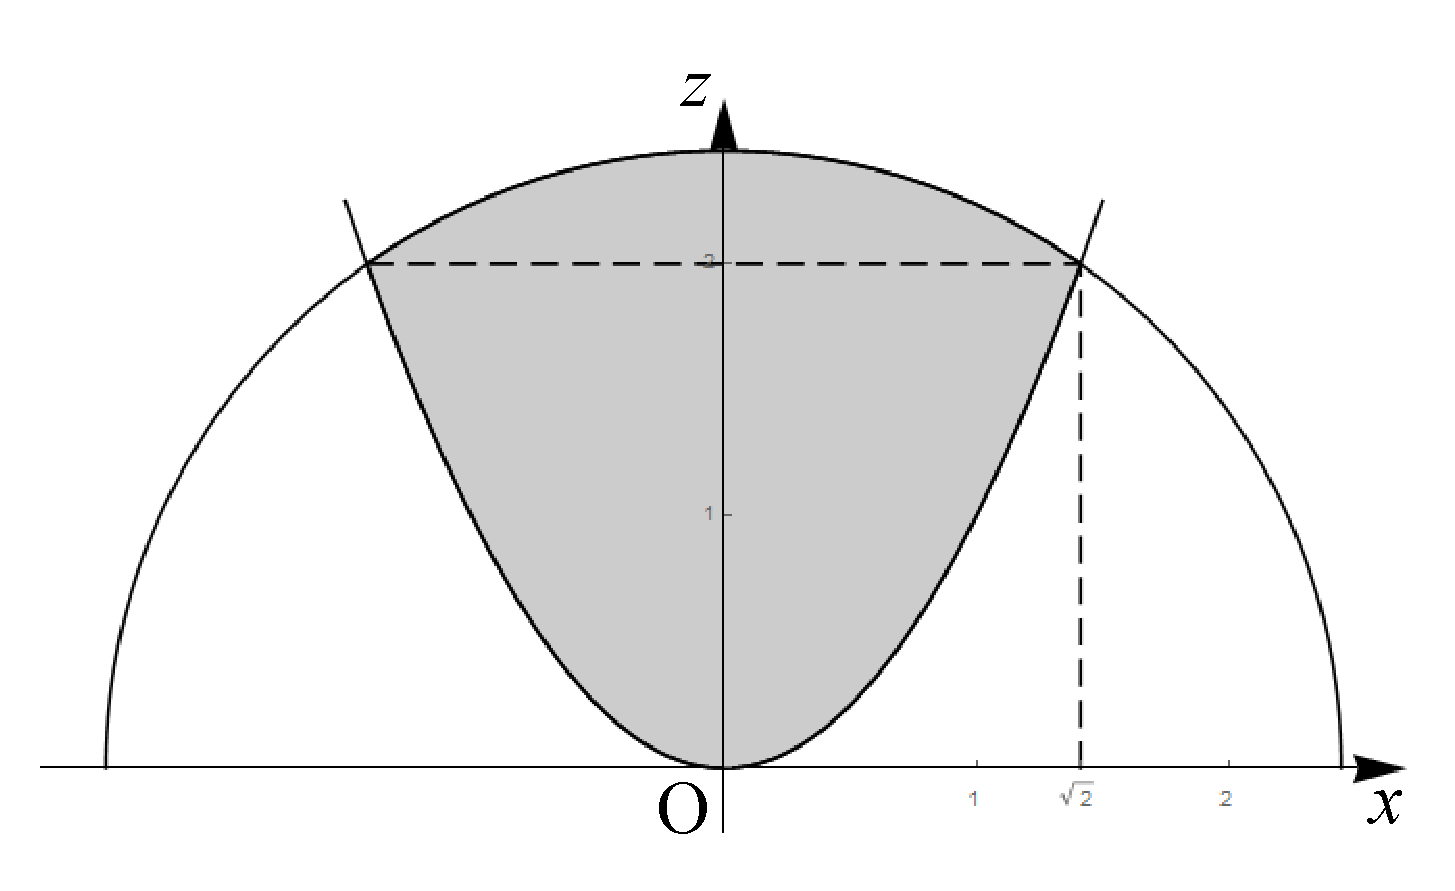
\includegraphics[height=0.3\textheight]{Figures19/Fig12-4-13-1.pdf} }}
\end{center}
\caption{习题12.4 13.题图示}
\label{12-4-13}
\end{figure}

解:由$\begin{cases}
z=x^2+y^2,\\
z=\sqrt{6-x^2-y^2},
\end{cases}$得$\begin{cases}
z=2,\\
x^2+y^2=2,
\end{cases}$该空间图形可表示为\\
$\Omega=\Set{(x,y)}{0\leqslant z\leqslant2,x^2+y^2\leqslant z}\cup\Set{(x,y)}{2\leqslant z\leqslant\sqrt6,x^2+y^2\leqslant6-z^2}$,

$\therefore\IIInt\Omega{}V=\Int02{}z\varIInt{\Omega_z}{}xy+\Int2{\sqrt6}{}z\varIInt{\Omega_z}{}xy=\Int02{\pi z}z+\Int2{\sqrt6}{\pi(6-z^2)}z\\
=\pi\frac12z^2\big|_0^2+\pi(6z-\frac13z^3)\big|_2^{\sqrt6}=2\pi+\pi(6\sqrt6-\frac13\cdot6\sqrt6-12+\frac83)=\pi(4\sqrt6-\frac{22}3)$.
%
%注:如图~\ref{12-4-13}所示.
%\begin{figure}[H]
%\begin{center}
%\includegraphics[height=0.4\textheight]{Figures19/Fig12-4-13.pdf}
%\end{center}
%\caption{习题12.4 13.题积分域在$xOz$平面上的截面图形}
%\label{12-4-13}
%\end{figure}

\item利用三重积分计算曲面所围成的空间区域的体积:\\
(1)$1\leqslant x^2+y^2\leqslant2x,0\leqslant z\leqslant xy$;\\
(2)$x^2+y^2+z^2=a^2,x^2+y^2+z^2=b^2,x^2+y^2=z^2,z\geqslant0,0<a<b$.

解:(1)
\begin{figure}[H]
\begin{center}
\subfloat[积分域]{\label{12-4-14-1-1}
{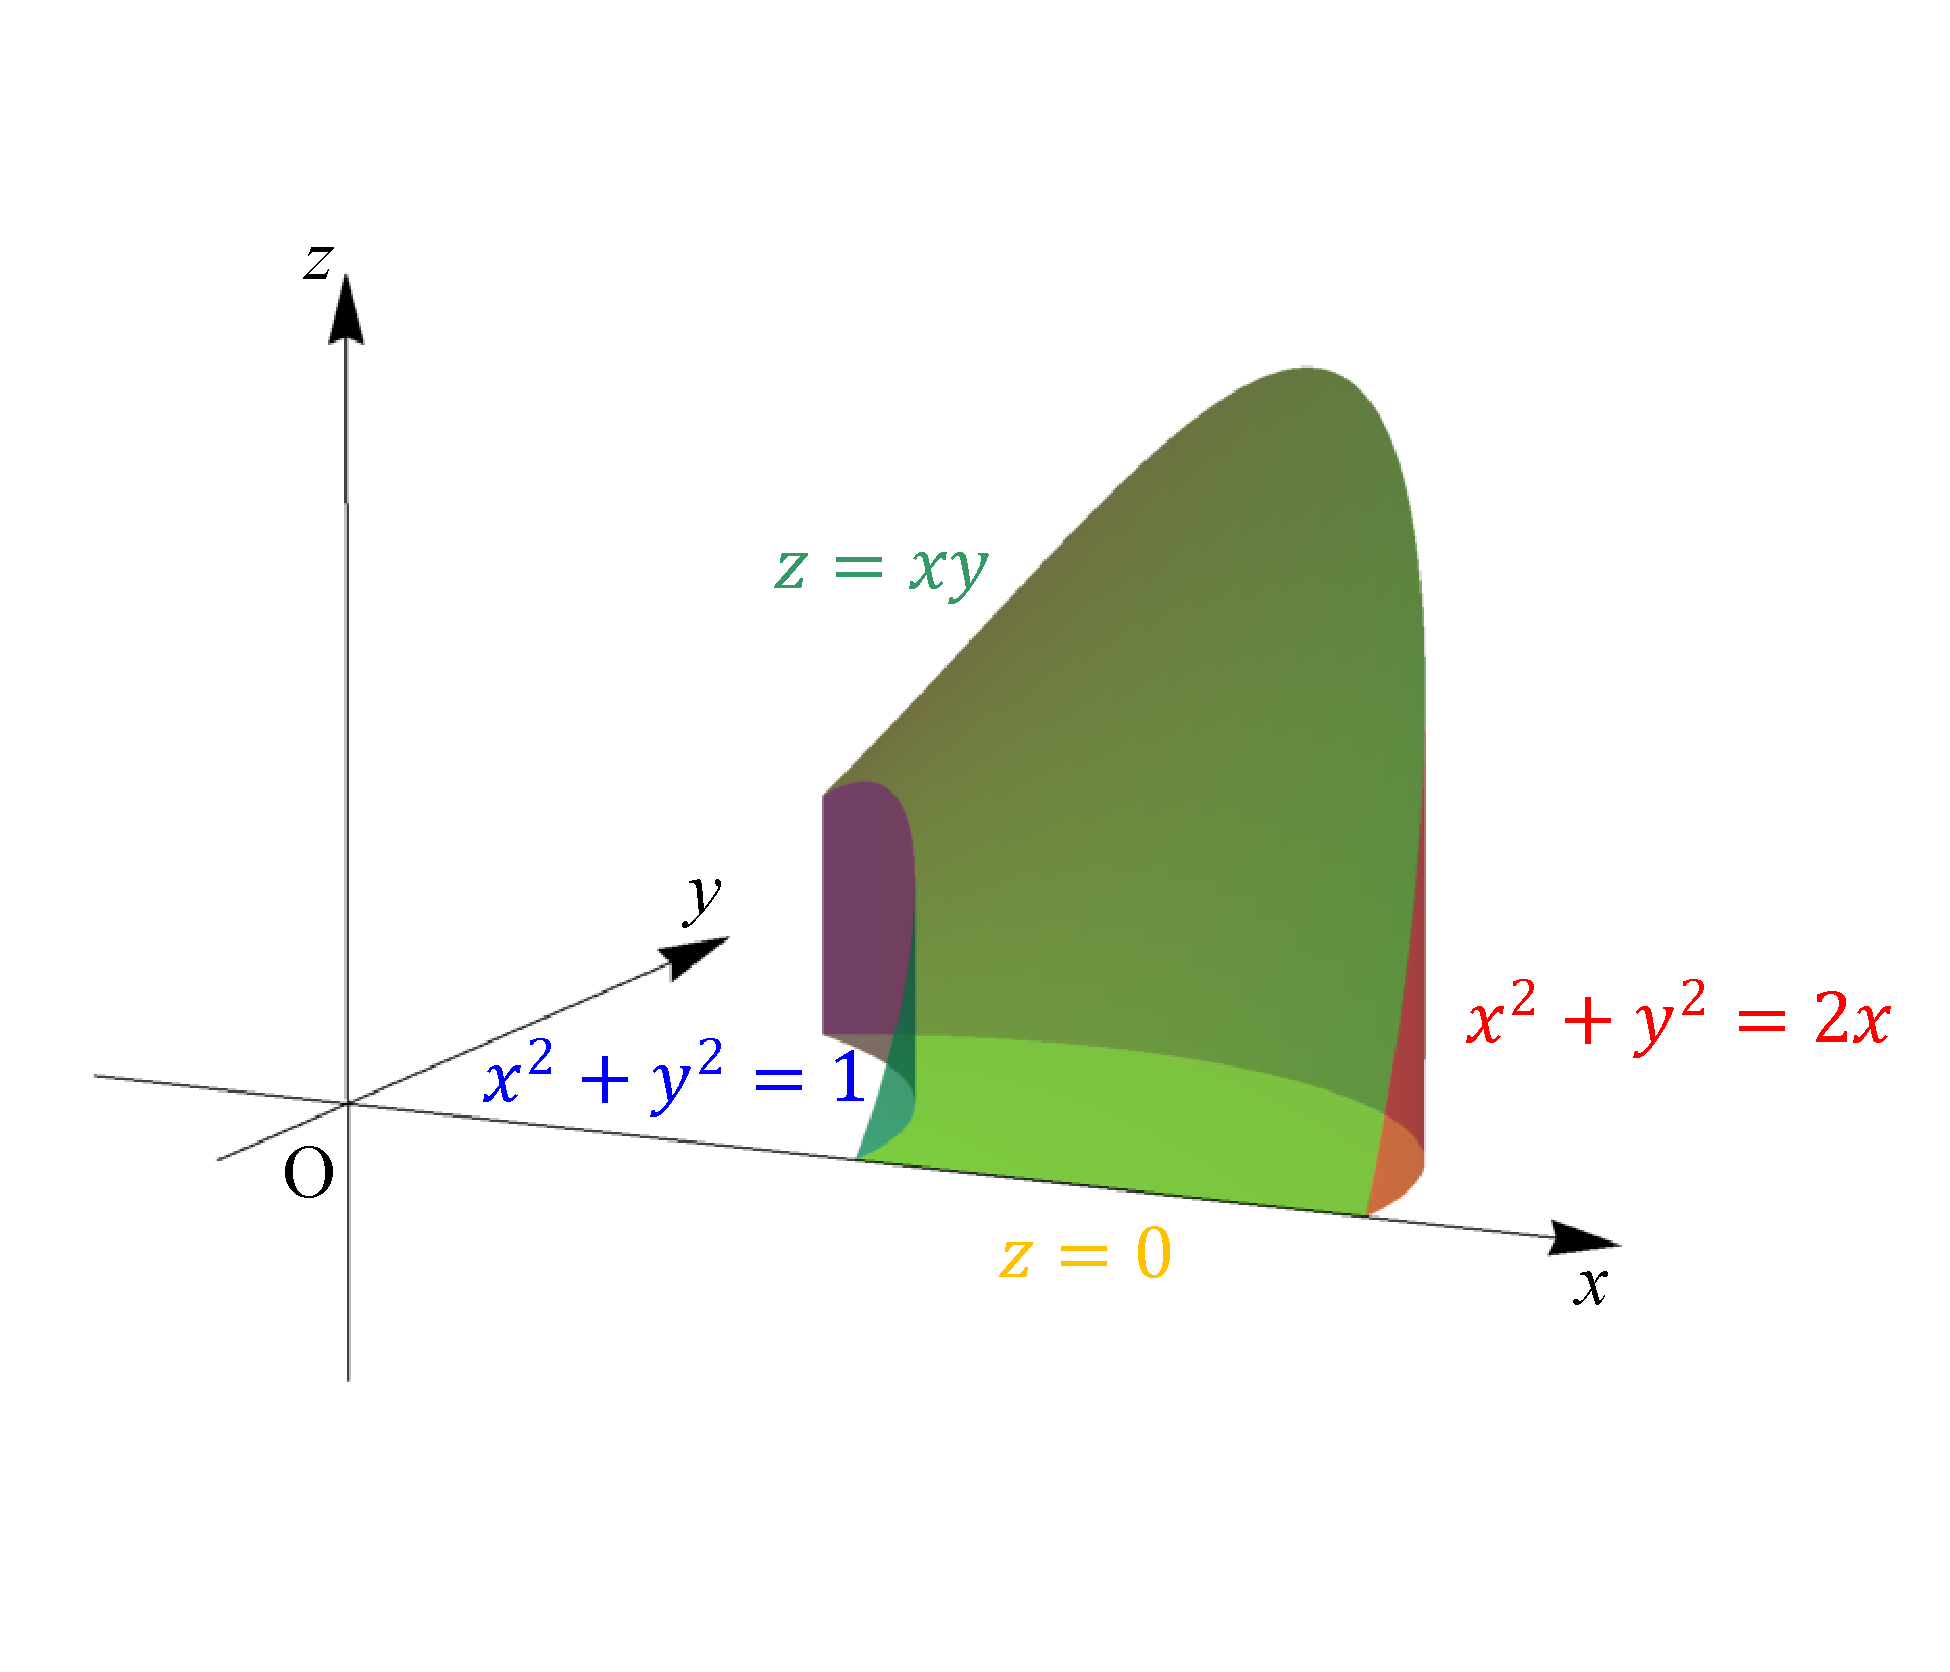
\includegraphics[height=0.5\textheight]{Figures19/Fig12-4-14-1-1.pdf} }}\\
\subfloat[积分域在$xOy$平面上的投影]{\label{12-4-14-1-1}
{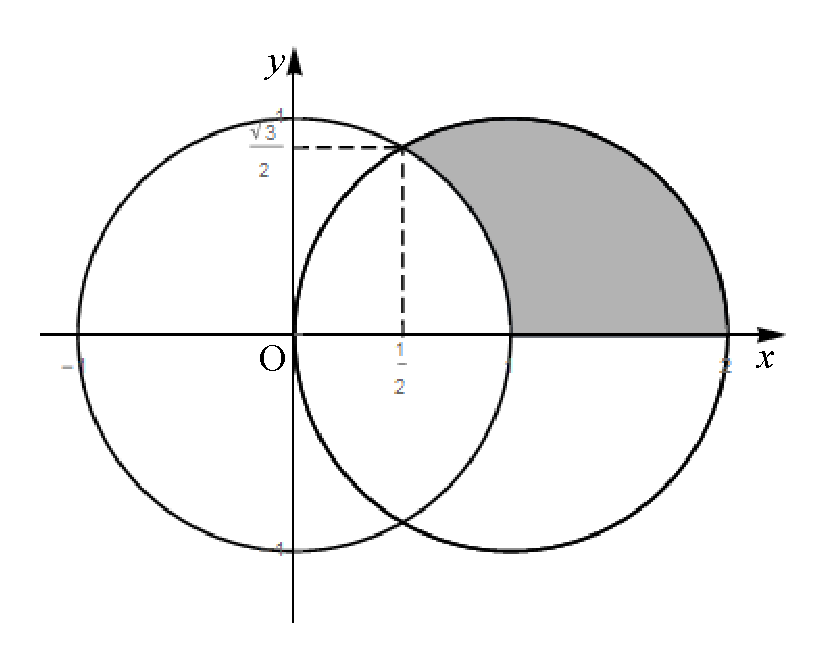
\includegraphics[height=0.4\textheight]{Figures19/Fig12-4-14-1-2.pdf} }}
\end{center}
\caption{习题12.4 14.(1)题图示}
\label{12-4-14-1}
\end{figure}

$\because0\leqslant z\leqslant xy$,

$\therefore xy\geqslant0$,

$\therefore$区域$\Omega=\Set{(x,y)}{1\leqslant x^2+y^2\leqslant2x,0\leqslant z\leqslant xy}$在柱坐标系下可表示为\\
$\Omega=\Set{(r,\theta,z)}{0\leqslant z\leqslant r^2\sin\theta\cos\theta,1\leqslant r\leqslant2\cos\theta,0\leqslant\theta\leqslant\frac\pi3}$,

$\therefore\IIInt\Omega{}V=\Int0{\frac\pi3}{}\theta\Int1{2\cos\theta}{}r\Int0{r^2\sin\theta\cos\theta}{r}z=\Int0{\frac\pi3}{}\theta\Int1{2\cos\theta}{r^3\sin\theta\cos\theta}r\\
=\Int0{\frac\pi3}{\sin\theta\cos\theta\frac14r^4\big|_1^{2\cos\theta}}\theta=\Int0{\frac\pi3}{\sin\theta\cos\theta\frac14\cdot(16\cos^4\theta-1)}\theta\\
=4\Int0{\frac\pi3}{\cos^5\theta\sin\theta}\theta-\frac14\Int0{\frac\pi3}{\sin\theta\cos\theta}\theta=-4\cdot\frac16\cos^6\theta\big|_0^{\frac\pi3}-\frac14\cdot\frac12\sin^2\theta\big|_0^{\frac\pi3}\\
=\frac23(1-\frac1{64})-\frac18\cdot\frac34=\frac9{16}$.
%
%注:如图~\ref{12-4-14-1}所示.
%\begin{figure}[H]
%\begin{center}
%\includegraphics[height=0.4\textheight]{Figures19/Fig12-4-14-1.pdf}
%\end{center}
%\caption{习题12.4 14.(1)题积分域在$xOy$平面上的投影}
%\label{12-4-14-1}
%\end{figure}

(2)
\begin{figure}[H]
\begin{center}
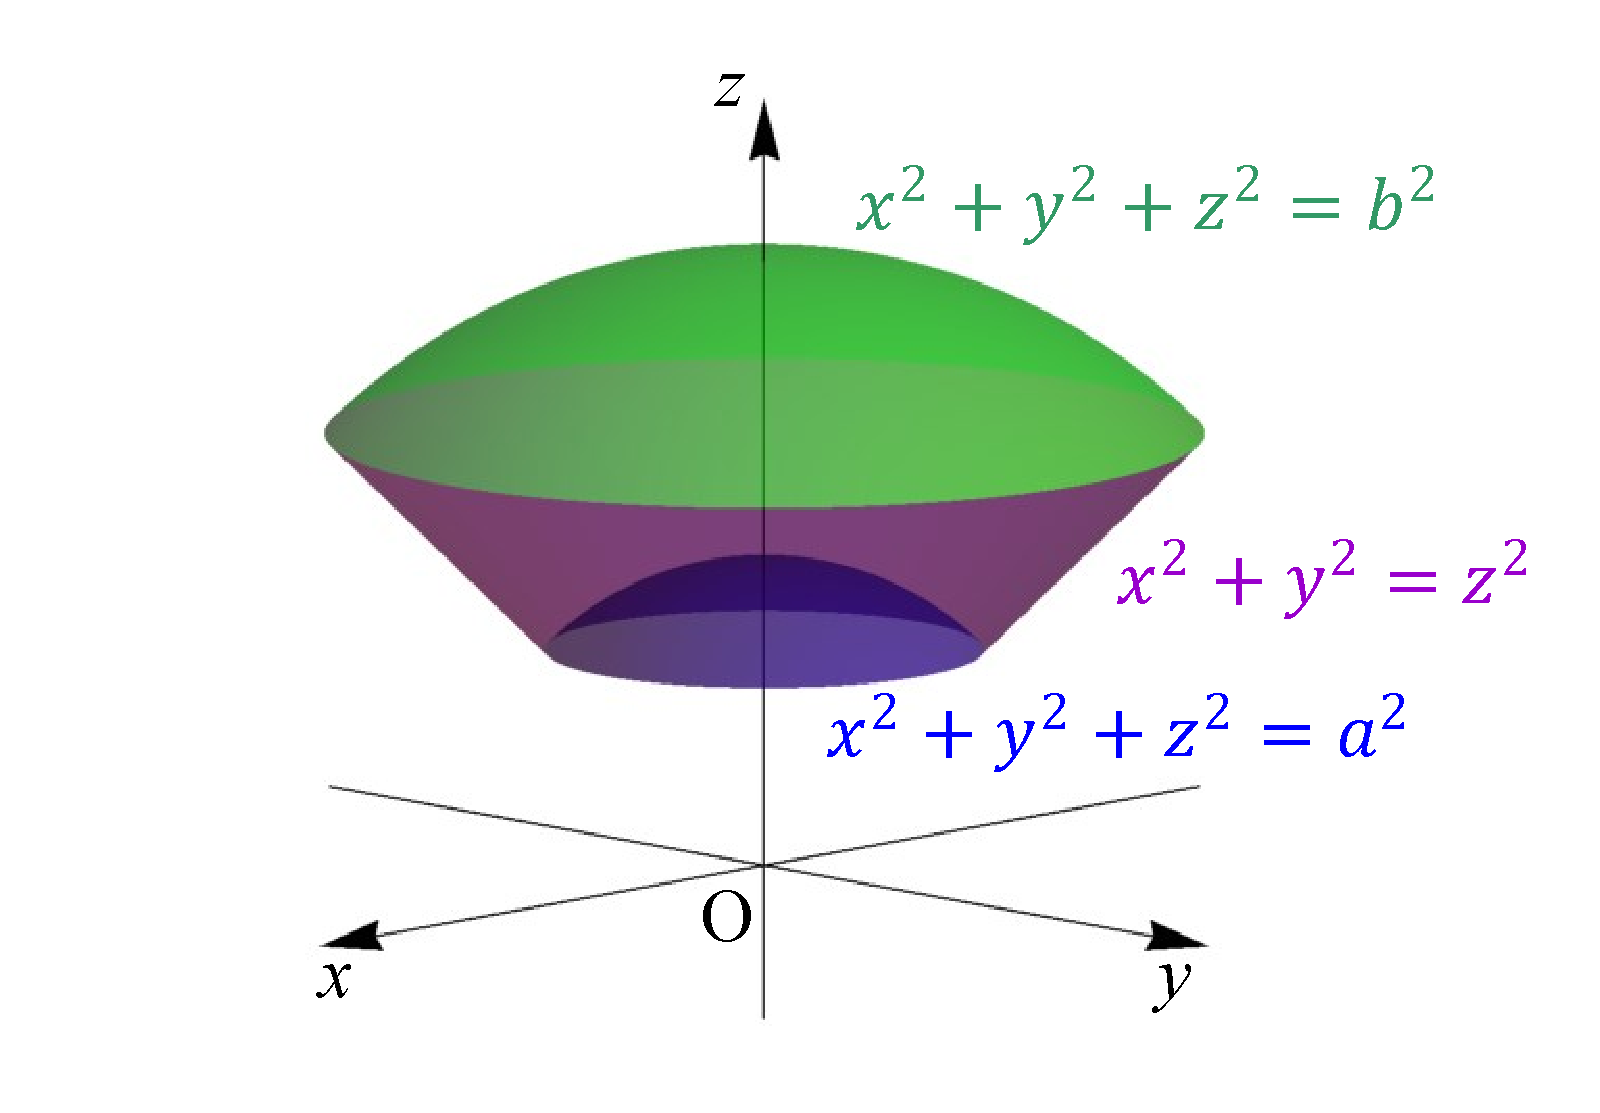
\includegraphics[height=0.4\textheight]{Figures19/Fig12-4-14-2.pdf}
\end{center}
\caption{习题12.4 14.(2)题积分域}
\label{12-4-14-2}
\end{figure}

已知区域$\Omega$在球坐标系下可表示为$\Omega=\Set{(r,\theta,\varphi)}{a\leqslant r\leqslant b,0\leqslant\theta\leqslant2\pi,0\leqslant\varphi\leqslant\frac\pi4}$,

$\therefore\IIInt\Omega{}V=\Int0{2\pi}{}\theta\Int0{\frac\pi4}{}\varphi\Int ab{r^2\sin\varphi}r=\Int0{2\pi}{}\theta\Int0{\frac\pi4}{\frac13r^3\big|_a^b\sin\varphi}\varphi=\frac23\pi(b^3-a^3)\Int0{\frac\pi4}{\sin\varphi}\varphi\\
=\frac23\pi(b^3-a^3)(-\cos\varphi)\big|_0^{\frac\pi4}=\frac23(1-\frac{\sqrt2}2)\pi(b^3-a^3)$.

\item求由平面$a_1x+b_1y+c_1z=\pm h_1,a_2x+b_2y+c_2z=\pm h_2,a_3x+b_3y+c_3z=\pm h_3$所围成平行六面体的体积.

解:令$\begin{cases}
u=a_1x+b_1y+c_1z,\\
v=a_2x+b_2y+c_2z,\\
w=a_3x+b_3y+c_3z,
\end{cases}$不妨设$h_1>0,h_2>0,h_3>0$,则该平行六面体可表示为$\Omega=\Set{(u,v,w)}{-h_1\leqslant u\leqslant h_1,-h_2\leqslant v\leqslant h_2,-h_3\leqslant w\leqslant h_3}$,

$\frac{\mathrm D(u,v,w)}{\mathrm D(x,y,z)}=\begin{vmatrix}
a_1&b_1&c_1\\
a_2&b_2&c_2\\
a_3&b_3&c_3
\end{vmatrix}=\det A$,

当$\det A\neq0$时,\\
$\varIIInt\Omega{}xyz=\varIIInt\Omega{|\frac{\mathrm D(x,y,z)}{\mathrm D(u,v,w)}|}uvw=\varIIInt\Omega{\frac1{|\frac{\mathrm D(u,v,w)}{\mathrm D(x,y,z)}|}}uvw=\varIIInt\Omega{\frac1{|\det A|}}uvw\\
=\frac1{|\det A|}\varIIInt\Omega{}uvw=\frac{2h_1\cdot2h_2\cdot2h_3}{|\det A|}=\frac{8h_1h_2h_3}{|\det A|}$.

\item设$D=\Set{(x,y)}{4\leqslant x^2+y^2\leqslant9}$是一平面圆环,每点的质量密度为$\mu(x,y)=1+x^2+y^2$,试求:\\
(1)$D$在第一象限部分的重心;\\
(2)$D$关于$y$轴的转动惯量.

\begin{figure}[H]
\begin{center}
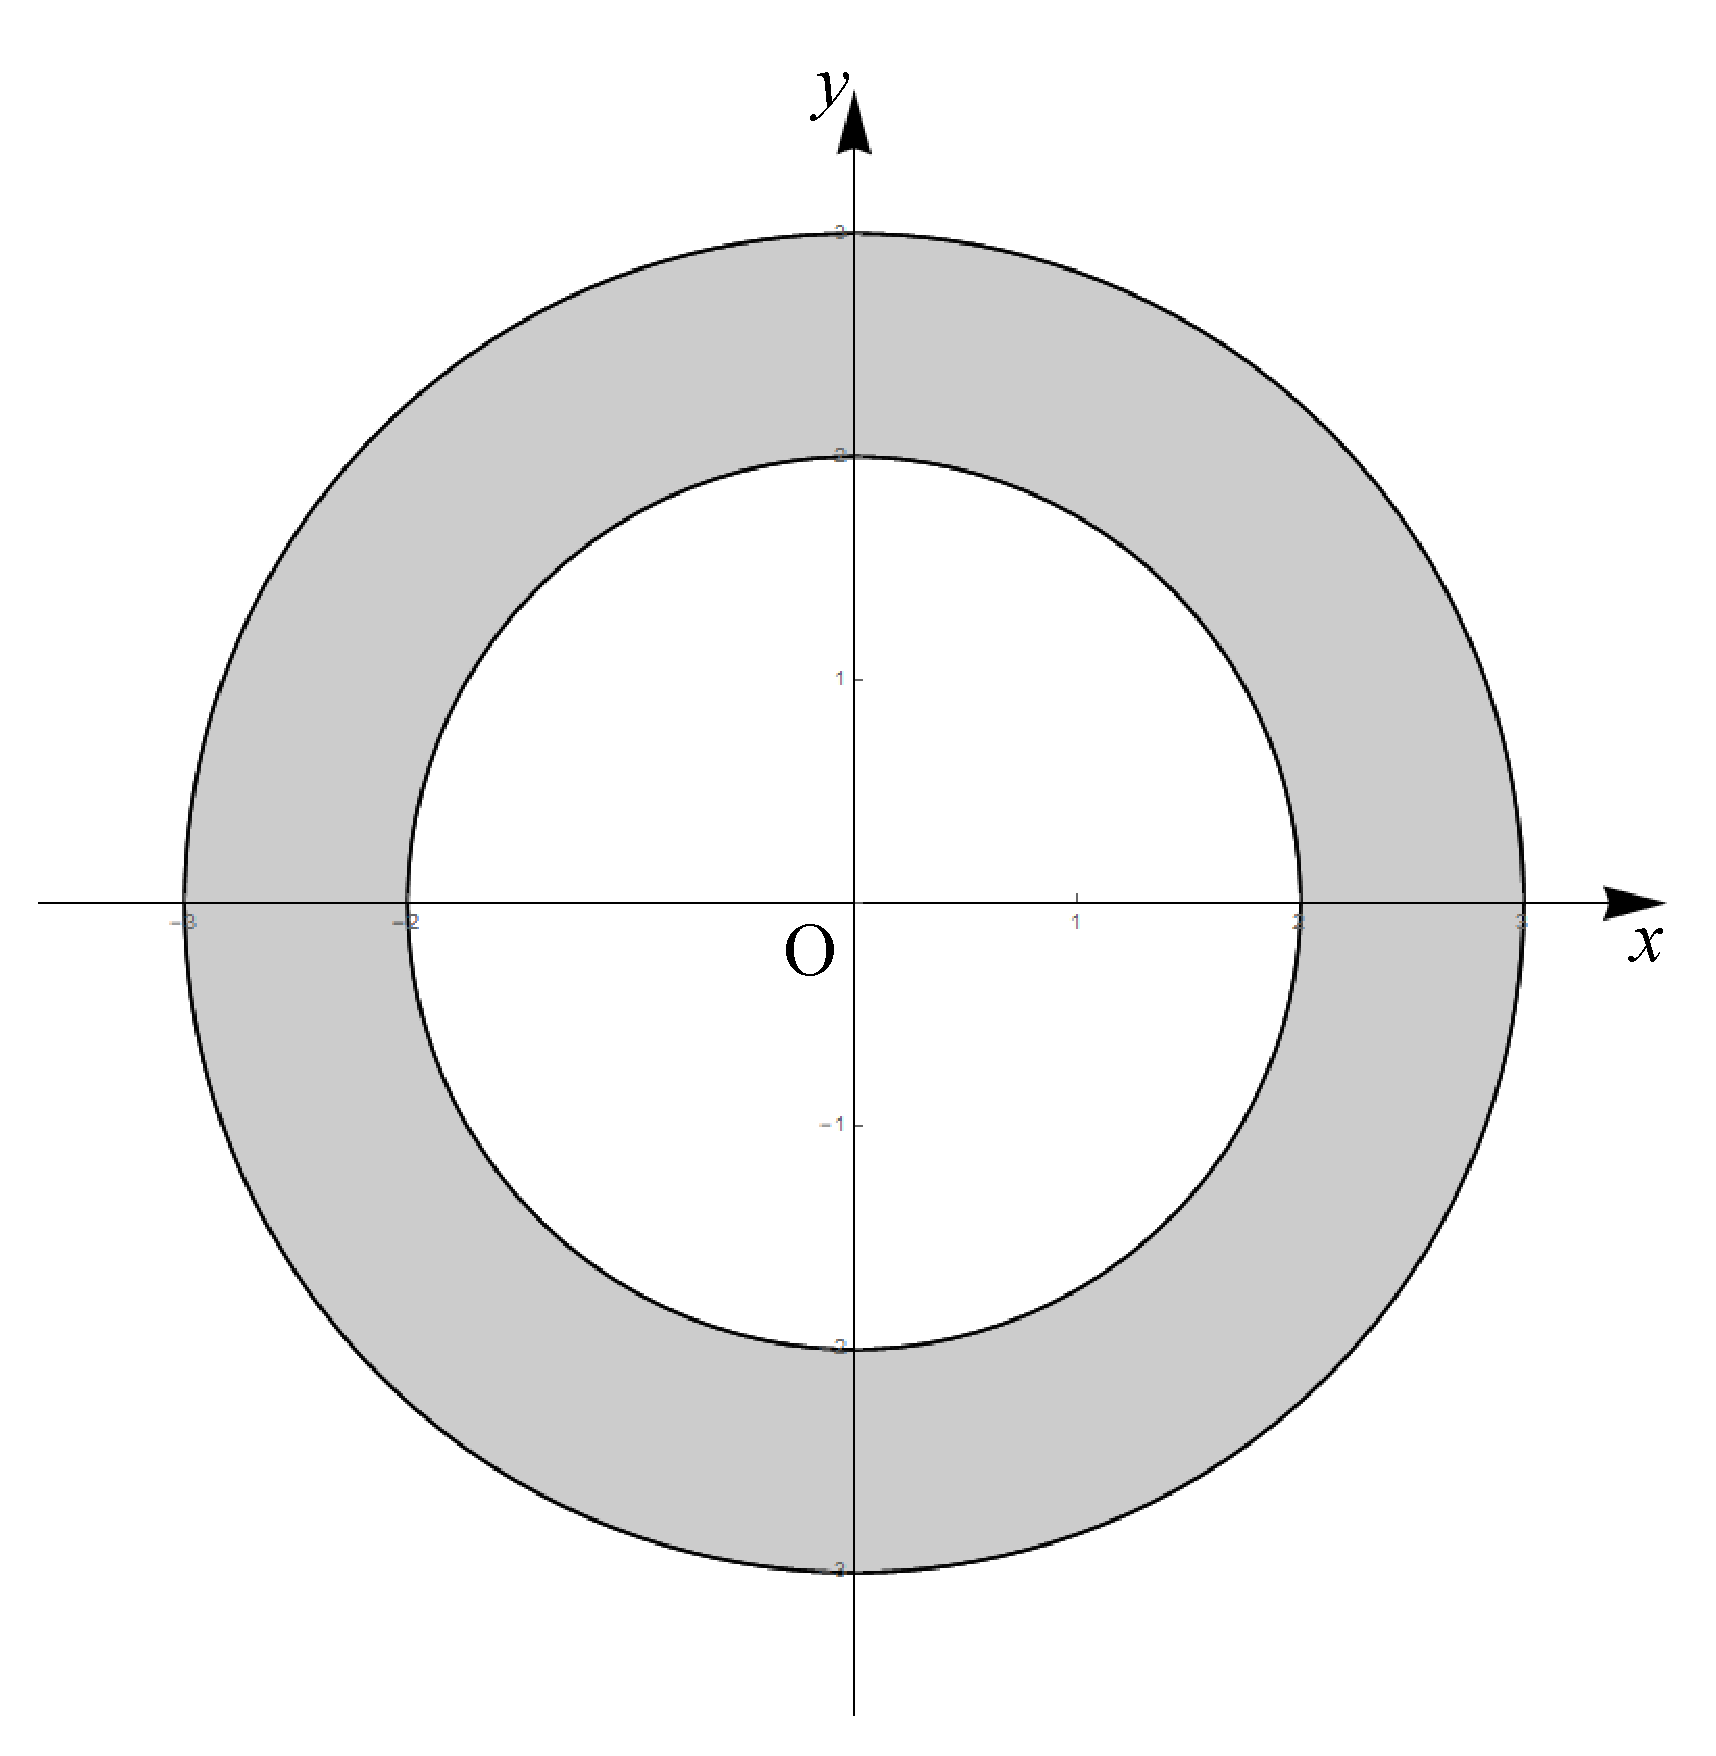
\includegraphics[height=0.4\textheight]{Figures19/Fig12-4-16.pdf}
\end{center}
\caption{习题12.4 16.题图示}
\label{12-4-16}
\end{figure}

解:(1)$D$在第一象限部分用极坐标表示为$D_1=\Set{(r,\theta)}{2\leqslant r\leqslant3,0\leqslant\theta\leqslant\frac\pi2}$,

$\therefore\bar{x}=\frac{\varIInt{D_1}{x\mu(x,y)}xy}{\varIInt{D_1}{\mu(x,y)}xy}=\frac{\Int0{2\pi}{}\theta\Int23{r\cos\theta(1+r^2)r}r}{\Int0{2\pi}{}\theta\Int23{(1+r^2)r}r}=\frac{\Int0{\frac\pi2}{\cos\theta}\theta\Int23{(r^2+r^4)}r}{\frac\pi2(\frac12r^2+\frac14r^4)\big|_2^3}=\frac{1\cdot(\frac13r^3+\frac15r^5)\big|_2^3}{\frac\pi2(\frac92+\frac{81}4-2-4)}=\frac{9+\frac{243}5-\frac83-\frac{32}5}{\frac\pi2(\frac{99}4-6)}\\
=\frac{5824}{1125\pi}$,

由对称性可知$\bar{y}=\bar{x}$,故$D$在第一象限部分的重心为$(\frac{5824}{1125\pi},\frac{5824}{1125\pi})$.

(2)$D$关于$y$轴的转动惯量\\
$J_y=\varIInt D{x^2\mu(x,y)}xy=\Int0{2\pi}{}\theta\Int23{r^2\cos^2\theta(1+r^2)r}r=\Int0{2\pi}{\cos^2\theta}\theta\Int23{(r^3+r^5)}r\\
=4\Int0{\frac\pi2}{\cos^2\theta}\theta(\frac14r^4+\frac16r^6)\big|_2^3=4\cdot\frac\pi4(\frac14\cdot81+\frac16\cdot729-4-\frac16\cdot64)=\frac{1525}{12}\pi$.

\item设球$x^2+y^2+z^2\leqslant2az$中各点的密度为$\rho=\frac1{\sqrt{x^2+y^2+z^2}}$,求球的质量与质心.

\begin{figure}[H]
\begin{center}
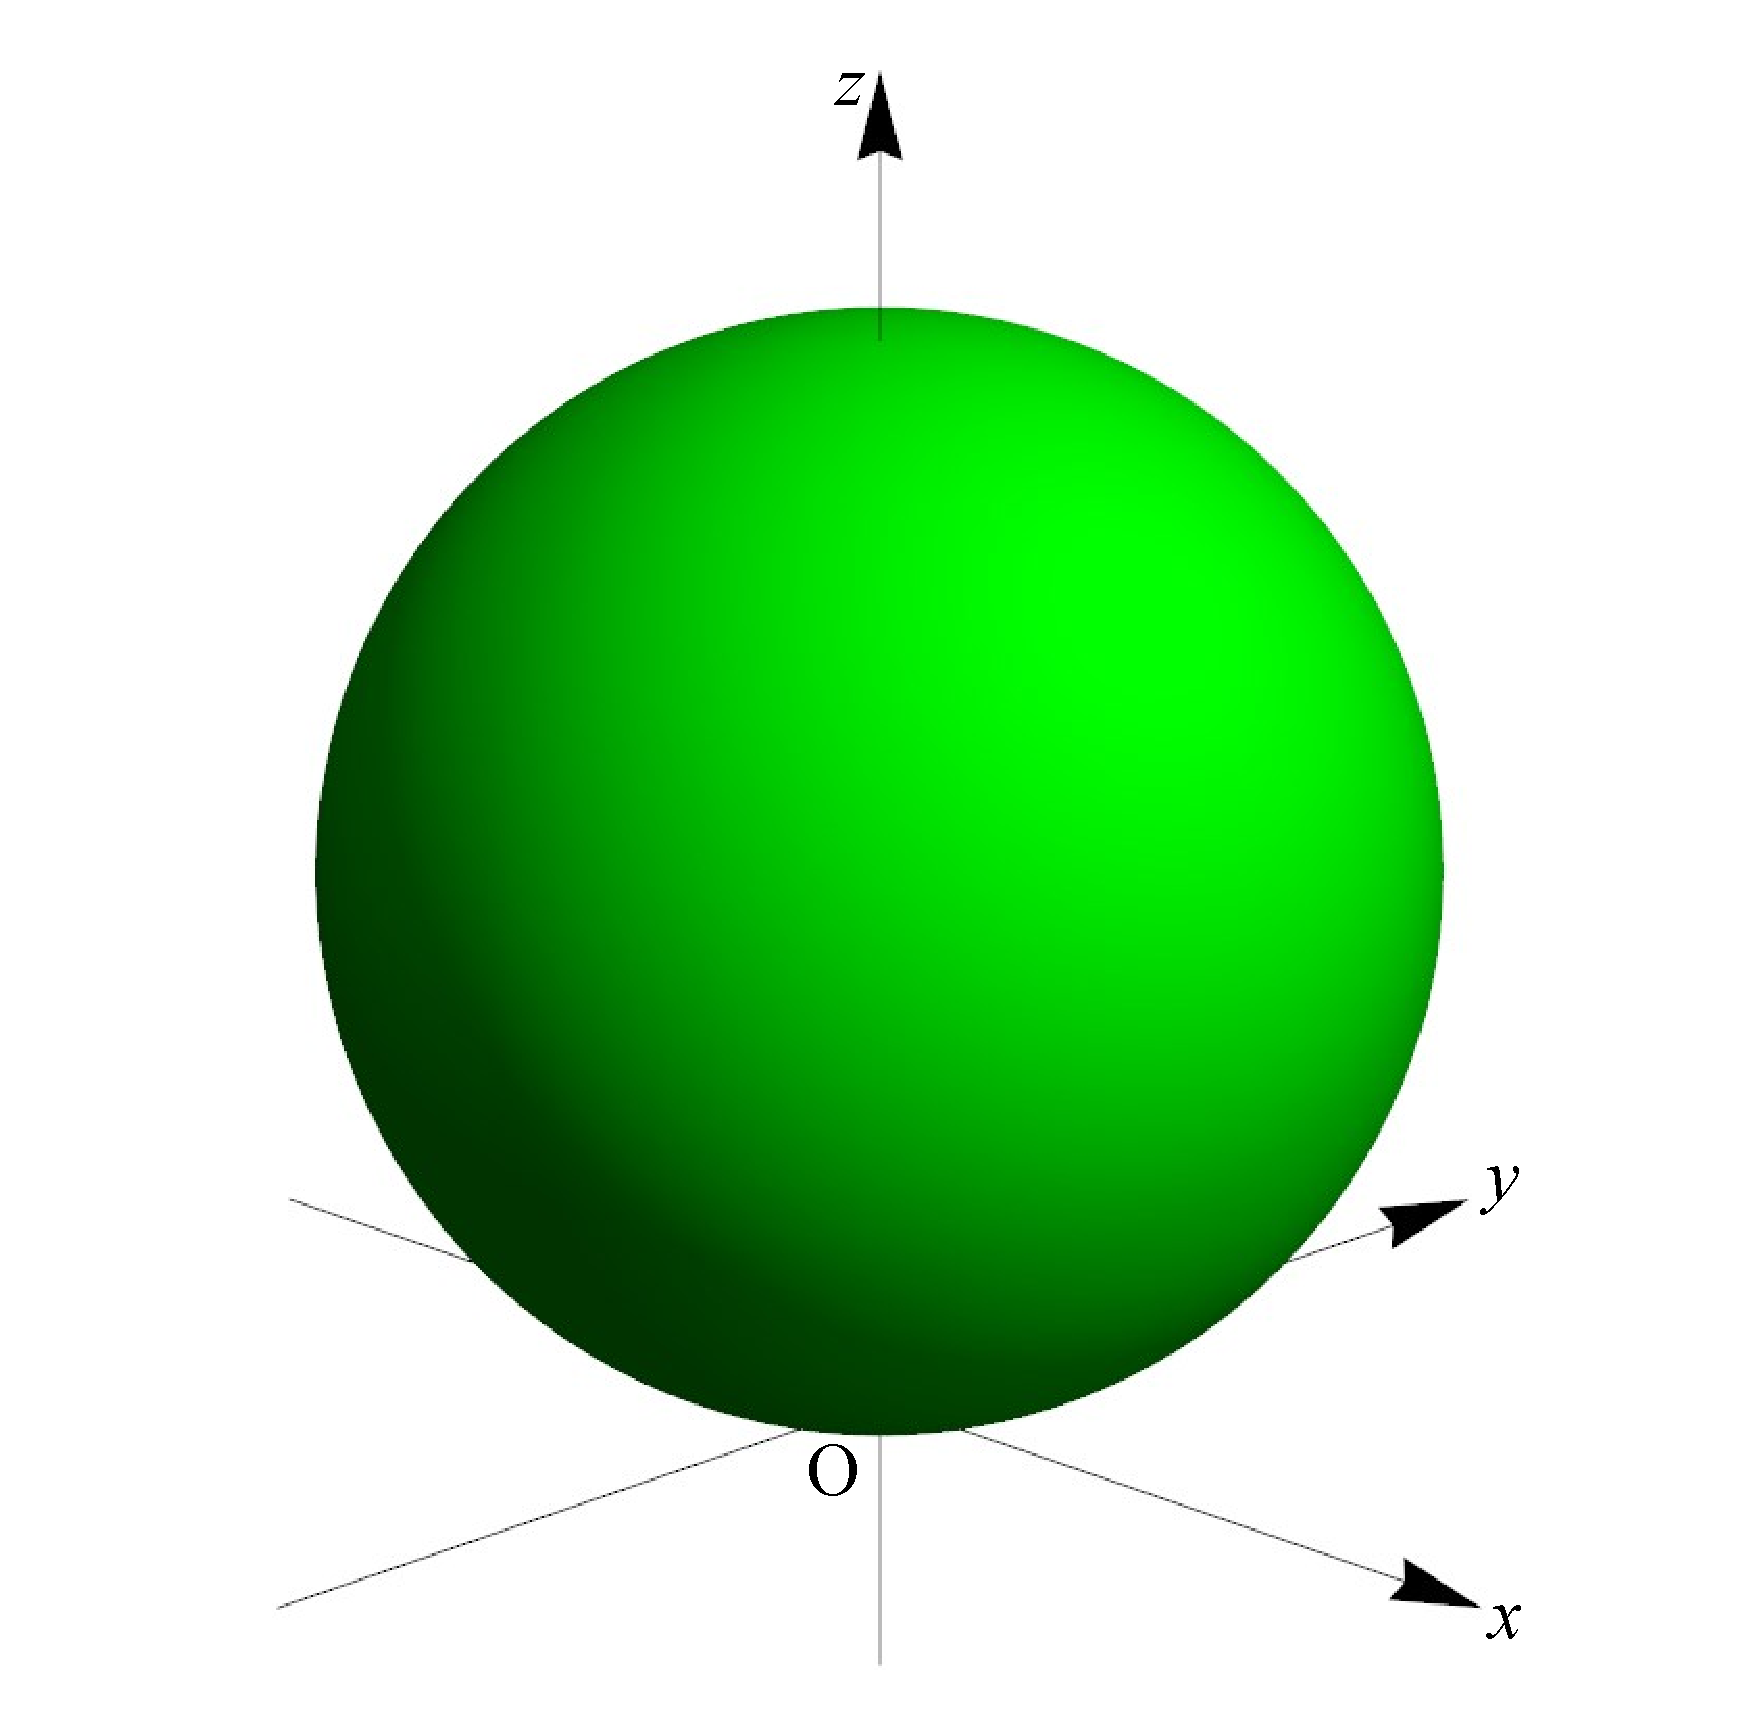
\includegraphics[height=0.4\textheight]{Figures19/Fig12-4-17.pdf}
\end{center}
\caption{习题12.4 17.题图示}
\label{12-4-17}
\end{figure}

解:该球用球坐标表示为$\Omega=\Set{(r,\theta,\varphi)}{0\leqslant r\leqslant2a\cos\varphi,0\leqslant\varphi\leqslant\frac\pi2,0\leqslant\theta\leqslant2\pi}$,

质量$m=\IIInt\Omega\rho V=\Int0{2\pi}{}\theta\Int0{\frac\pi2}{}\varphi\Int0{2a\cos\varphi}{\frac1rr^2\sin\varphi}r=2\pi\Int0{\frac\pi2}{}\varphi(\frac12r^2\sin\varphi)\big|_0^{2a\cos\varphi}\\
=2\pi\Int0{\frac\pi2}{(\frac124a^2\cos^2\varphi\sin\varphi)}\varphi=-4\pi a^2\frac13\cos^3\varphi\big|_0^{\frac\pi2}=\frac43\pi a^2$,

由对称性可知$\bar{x}=\bar{y}=0$,

$M_{xy}=\IIInt\Omega{z\rho}V=\Int0{2\pi}{}\theta\Int0{\frac\pi2}{}\varphi\Int0{2a\cos\varphi}{r\cos\varphi\frac1rr^2\sin\varphi}r=2\pi\Int0{\frac\pi2}{}\varphi\cos\varphi\sin\varphi\frac13r^3\big|_0^{2a\cos\varphi}\\
=2\pi\Int0{\frac\pi2}{\frac83a^3\cos^4\varphi\sin\varphi}\varphi=-\frac{16}3\pi a^3\frac15\cos^5\varphi\big|_0^{\frac\pi2}=\frac{16}{15}\pi a^3$,

$\therefore\bar{z}=\frac{M_{xy}}m=\frac{\frac{16}{15}\pi a^3}{\frac43\pi a^2}=\frac45a$,

故质心为$(0,0,\frac45a)$.

\item设$\Omega$由$z=x^2+y^2$及$z=2x$围成,密度$\rho=y^2$,求它对$z$轴的转动惯量.

\begin{figure}[H]
\begin{center}
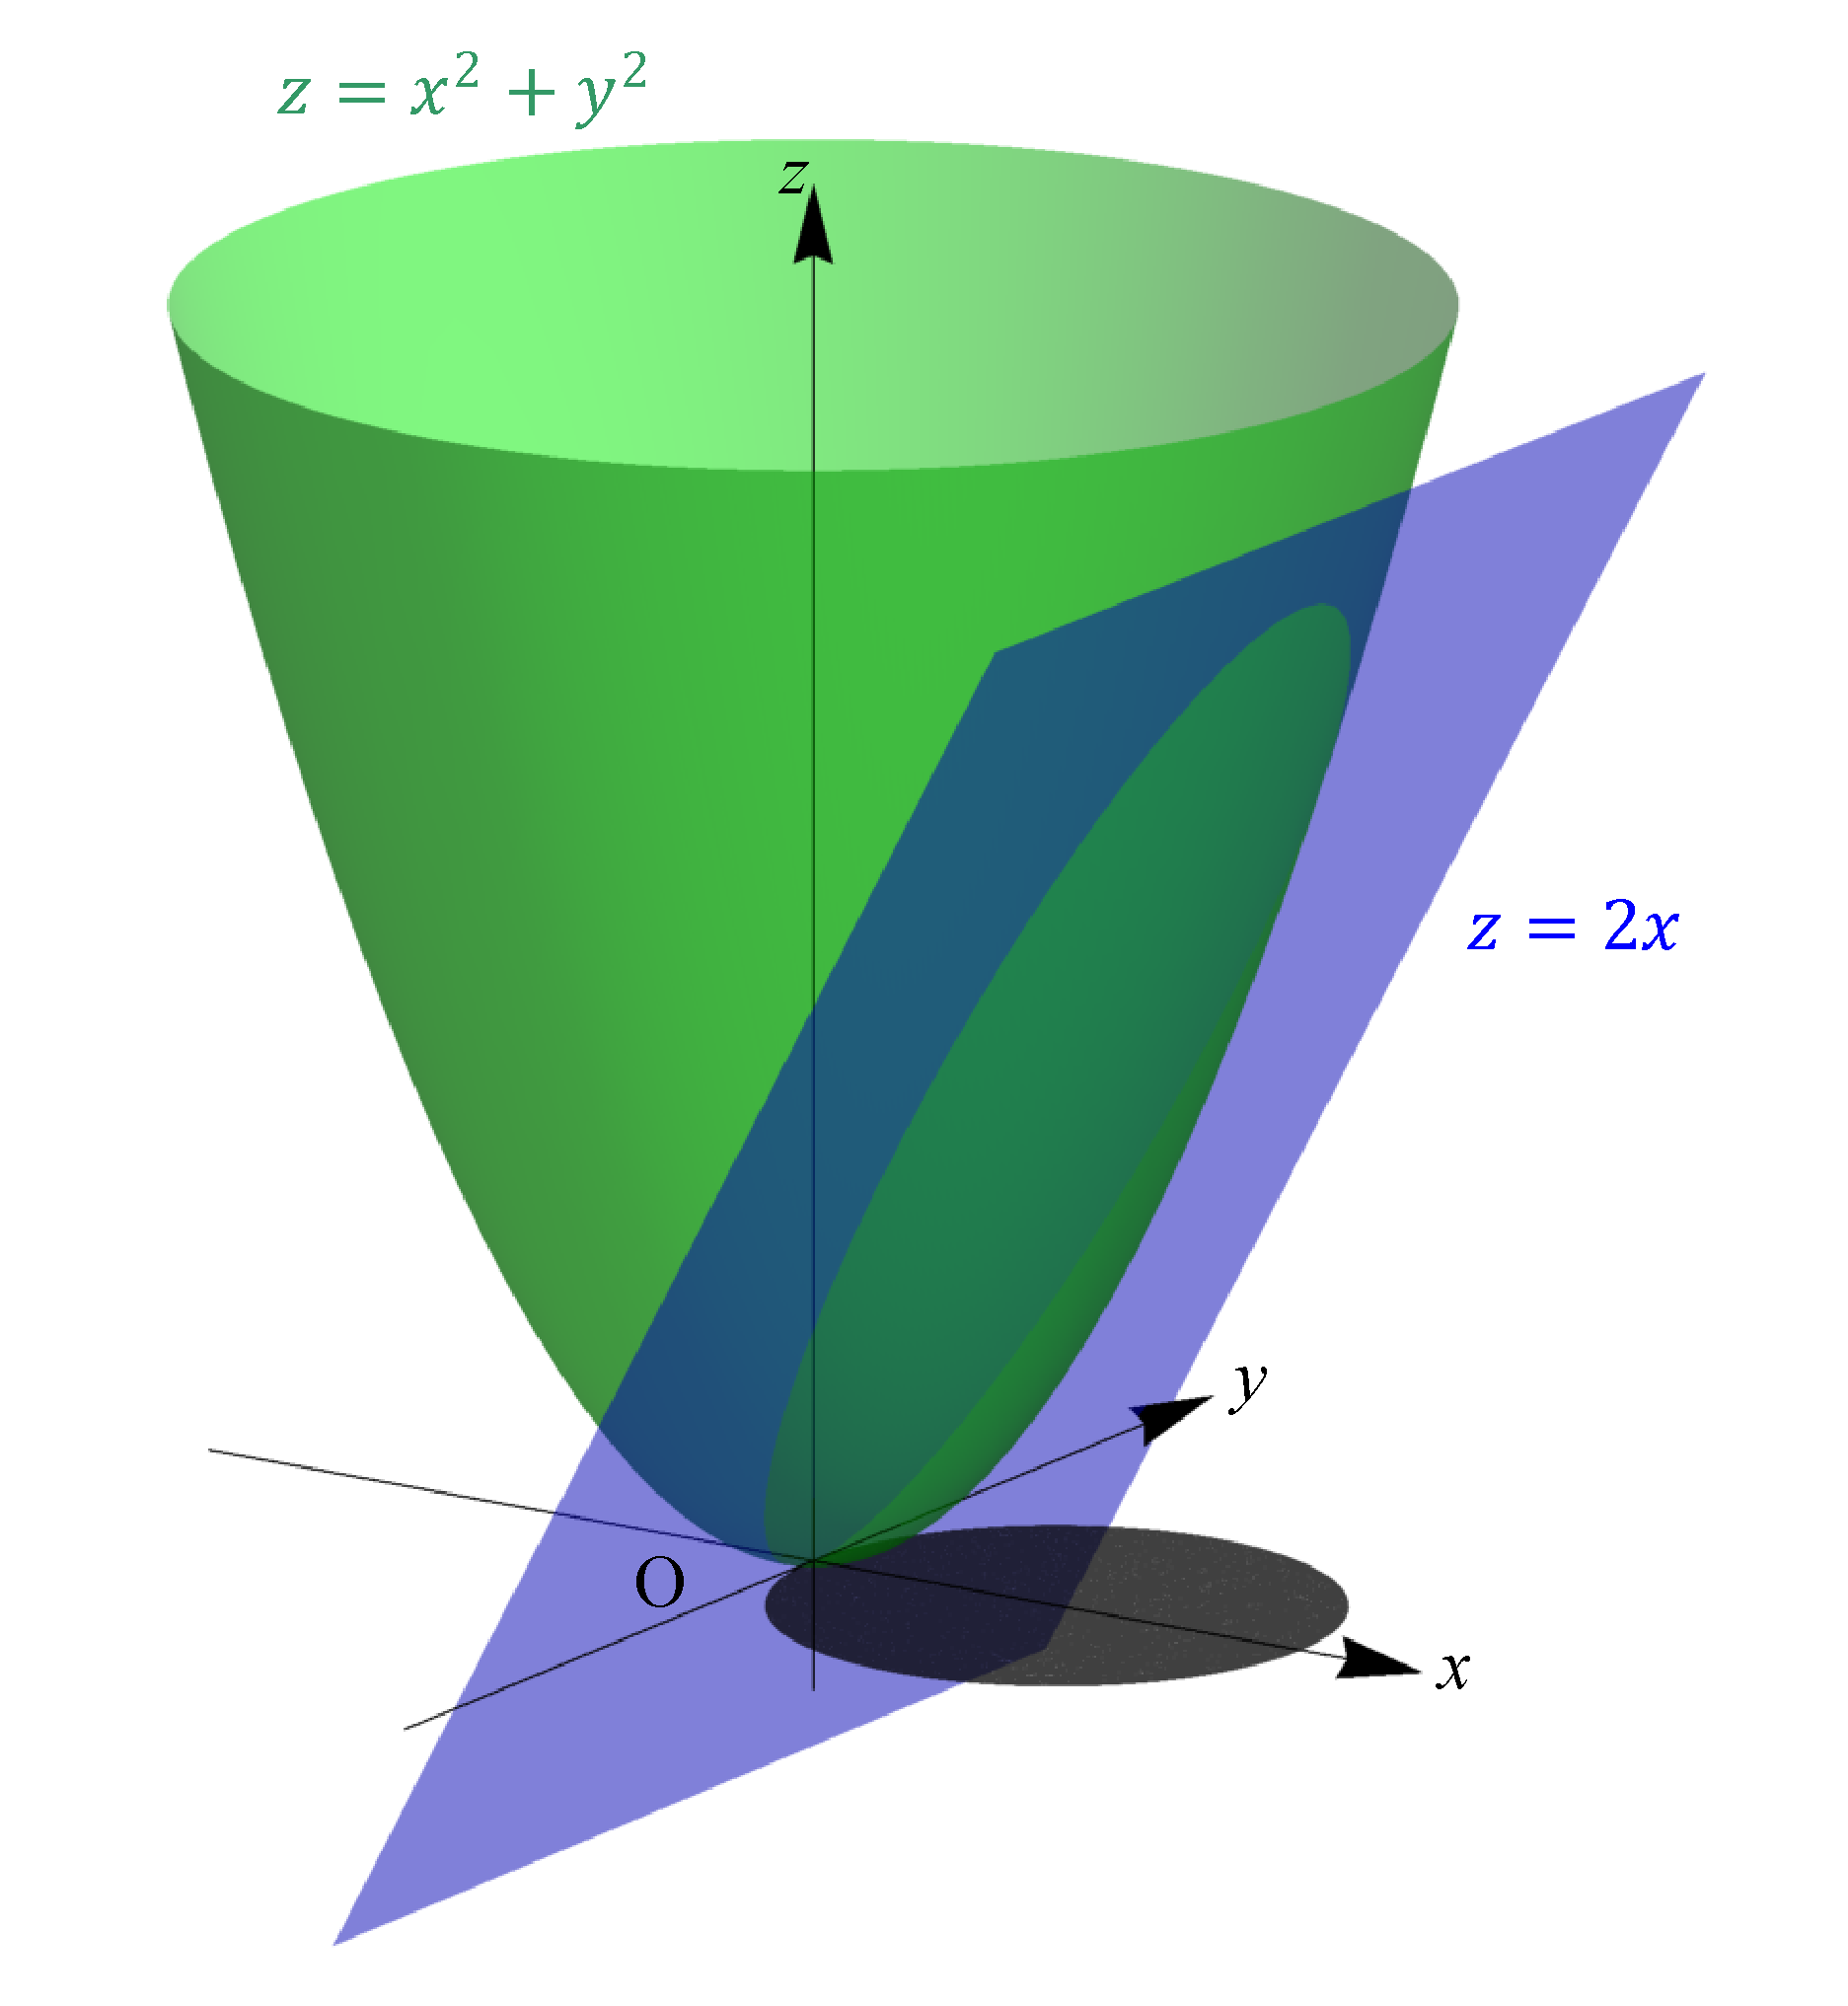
\includegraphics[height=0.4\textheight]{Figures19/Fig12-4-18.pdf}
\end{center}
\caption{习题12.4 18.题图示}
\label{12-4-18}
\end{figure}

解:由$\begin{cases}
z=x^2+y^2,\\
z=2x,
\end{cases}$得两曲面的投影柱面$x^2+y^2=2x$,

$\therefore$积分域在柱坐标系下表示为$\Omega=\Set{(r,\theta,z)}{r^2\leqslant z\leqslant 2r\cos\theta,0\leqslant r\leqslant2\cos\theta,-\frac\pi2\leqslant\theta\leqslant\frac\pi2}$,

$\therefore J_z=\varIIInt\Omega{(x^2+y^2)\rho}xyz=\Int{-\frac\pi2}{\frac\pi2}{}\theta\Int0{2\cos\theta}{}r\Int{r^2}{2r\cos\theta}{r^2r^2\sin^2\theta\cdot r}z\\
=\Int{-\frac\pi2}{\frac\pi2}{}\theta\Int0{2\cos\theta}{r^5\sin^2\theta(2r\cos\theta-r^2)}r=\Int{-\frac\pi2}{\frac\pi2}{}\theta\Int0{2\cos\theta}{(2r^6\sin^2\theta\cos\theta-r^7\sin^2\theta)}r\\
=\Int{-\frac\pi2}{\frac\pi2}{(\frac27r^7\sin^2\theta\cos\theta-\frac18r^8\sin^2\theta)\big|_0^{2\cos\theta}}\theta=\Int{-\frac\pi2}{\frac\pi2}{(\frac{2^8}7\cos^8\theta\sin^2\theta-\frac{2^8}8\cos^8\theta\sin^2\theta)}\theta\\
=\frac{2^8}{56}\cdot2\Int0{\frac\pi2}{\cos^8\theta\sin^2\theta}\theta=\frac{64}7\Int0{\frac\pi2}{\cos^8\theta(1-\cos^2\theta)}\theta=\frac{64}7(\Int0{\frac\pi2}{\cos^8\theta}\theta-\Int0{\frac\pi2}{\cos^{10}\theta}\theta)\\
=\frac{64}7(\frac{7\cdot5\cdot3\cdot1}{8\cdot6\cdot4\cdot2}\cdot\frac\pi2-\frac{9\cdot7\cdot5\cdot3\cdot1}{10\cdot8\cdot6\cdot4\cdot2}\cdot\frac\pi2)=\frac{64}7(\frac1{10}\cdot\frac{7\cdot5\cdot3\cdot1}{8\cdot6\cdot4\cdot2})\cdot\frac\pi2=\frac\pi8$.

\item试证曲面$z=x^2+y^2+a(a>0)$上任意点处的切平面与曲面$z=x^2+y^2$所围成的空间区域的体积是一常数.

\begin{figure}[H]
\begin{center}
\subfloat[积分域]{\label{12-4-19-1}
{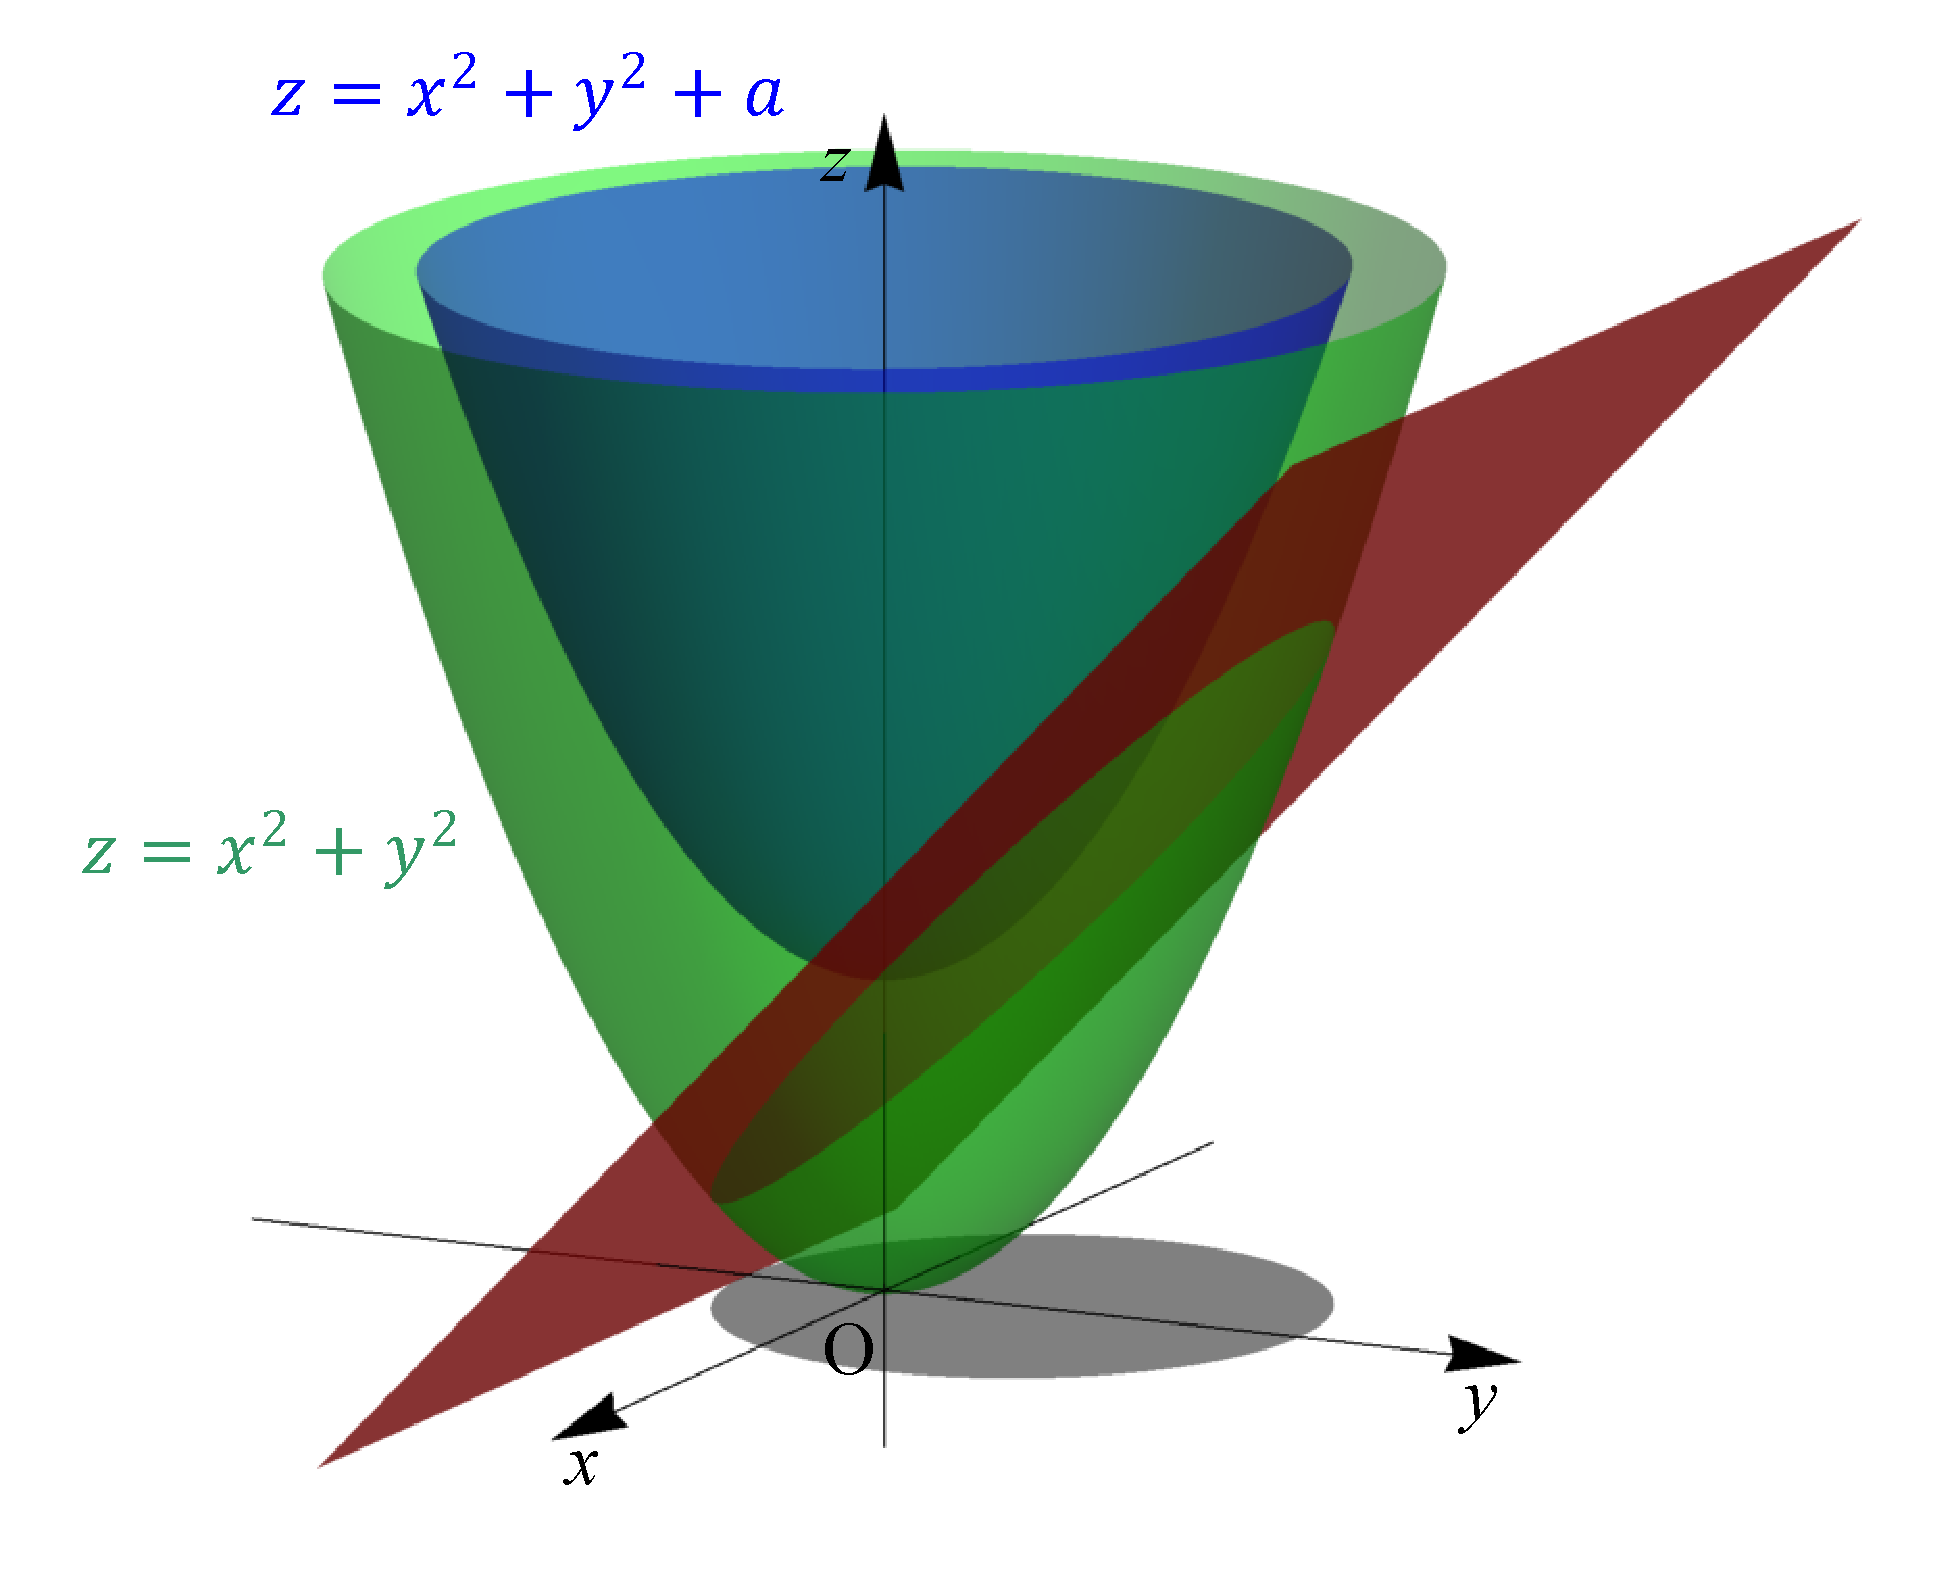
\includegraphics[height=0.5\textheight]{Figures19/Fig12-4-19-1.pdf} }}\\
\subfloat[积分域在$lOz$平面上的截面图形,$lOz$平面由$Oz$轴与切点确定.]{\label{12-4-19-2}
{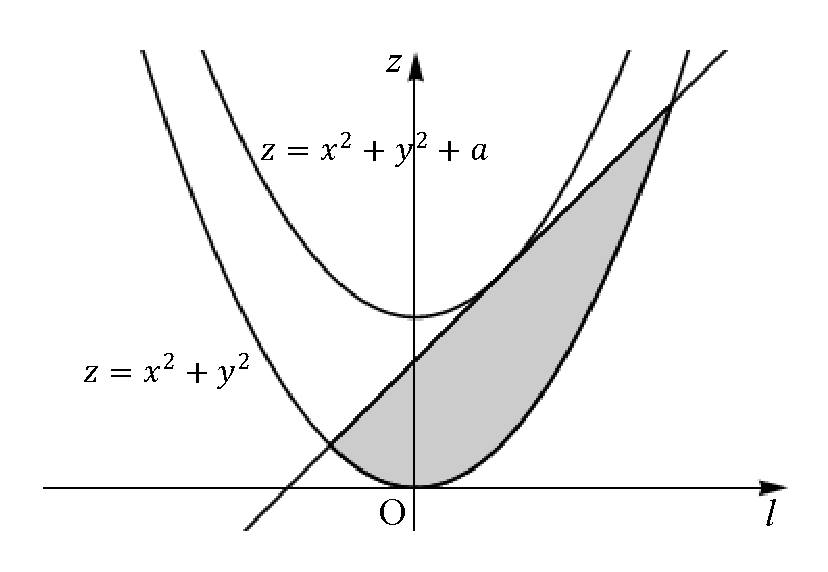
\includegraphics[height=0.4\textheight]{Figures19/Fig12-4-19-2.pdf} }}
\end{center}
\caption{习题12.4 19.题图示}
\label{12-4-19}
\end{figure}

证明:设$(x_0,y_0,z_0)$是曲面$z=x^2+y^2+a$上的任意点,则$z_0=x_0^2+y_0^2+a$,曲面在该点的法向量为$\bm n=(2x,2y,-1)\big|_{(x_0,y_0,z_0)}=(2x_0,2y_0,-1)$,

$\therefore$切平面的方程为$2x_0(x-x_0)+2y_0(y-y_0)-(z-z_0)=0$,\\
即$2x_0x+2y_0y-z=2x_0^2+2y_0^2-z_0=2(z_0-a)-z_0=z_0-2a$,

由$\begin{cases}
z=x^2+y^2,\\
2x_0x+2y_0y-z=z_0-2a,
\end{cases}$得切平面与曲面$z=x^2+y^2$的交线所在的投影柱面为$x^2+y^2-2x_0x-2y_0y+z_0-2a=0$,\\
即$(x-x_0)^2+(y-y_0)^2=x_0^2+y_0^2-z_0+2a=z_0-a-z_0+2a=a$,

令$\begin{cases}
x=x_0+r\cos\theta,\\
y=y_0+r\sin\theta,\\
z=z,
\end{cases}\frac{\mathrm D(x,y)}{\mathrm D(r,\theta)}=\begin{vmatrix}
\cos\theta&-r\sin\theta&0\\
\sin\theta&r\cos\theta&0\\
0&0&1
\end{vmatrix}=r$\\
切平面用$r,\theta,z$坐标表示为$2x_0(x_0+r\cos\theta)+2y_0(y_0+r\sin\theta)-z\\
=2x_0r\cos\theta+2y_0r\sin\theta-z+2x_0^2+2y_0^2=z_0-2a$,\\
即$z=2x_0r\cos\theta+2y_0r\sin\theta+2x_0^2+2y_0^2-z_0+2a\\
=2x_0r\cos\theta+2y_0r\sin\theta+2(z_0-a)-z_0+2a=2x_0r\cos\theta+2y_0r\sin\theta+z_0$,

曲面$z=x^2+y^2$用$r,\theta,z$坐标表示为$z=(x_0+r\cos\theta)^2+(y_0+r\sin\theta)^2\\
=r^2+2x_0r\cos\theta+2y_0r\sin\theta+x_0^2+y_0^2=r^2+2x_0r\cos\theta+2y_0r\sin\theta+z_0-a$,

$\therefore$所求空间区域$\Omega=\{(r,\theta,z)\ \vert\ 0\leqslant\theta\leqslant2\pi,0\leqslant r\leqslant\sqrt a,\\
2x_0r\cos\theta+2y_0r\sin\theta+z_0\leqslant z\leqslant r^2+2x_0r\cos\theta+2y_0r\sin\theta+z_0-a \}$,

$\therefore\varIIInt\Omega{}xyz=\varIIInt\Omega{|\frac{\mathrm D(x,y)}{\mathrm D(r,\theta)}|}r\theta z=\Int0{2\pi}{}\theta\Int0{\sqrt a}{}r\Int{r^2+2x_0r\cos\theta+2y_0r\sin\theta+z_0-a}{2x_0r\cos\theta+2y_0r\sin\theta+z_0}{r}z\\
=\Int0{2\pi}{}\theta\Int0{\sqrt a}{r[2x_0r\cos\theta+2y_0r\sin\theta+z_0-(r^2+2x_0r\cos\theta+2y_0r\sin\theta+z_0-a)]}r\\
=\Int0{2\pi}{}\theta\Int0{\sqrt a}{r(a-r^2)}r=2\pi(\frac12ar^2-\frac14r^4)\big|_0^{\sqrt a}=\frac\pi2 a^2$,

故曲面$z=x^2+y^2+a(a>0)$上任意点处的切平面与曲面$z=x^2+y^2$所围成的空间区域的体积是一常数.

%注:如图~\ref{12-4-19}所示.
%\begin{figure}[H]
%\begin{center}
%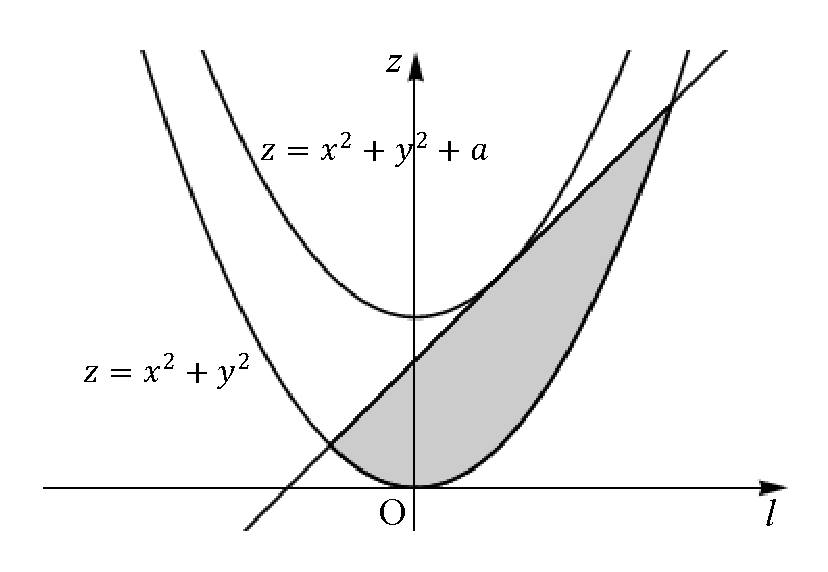
\includegraphics[height=0.3\textheight]{Figures19/Fig12-4-19-2.pdf}
%\end{center}
%\caption{习题12.4 19.题积分域在$lOz$平面上的截面图形,$lOz$平面由$Oz$轴与切点确定.}
%\label{12-4-19}
%\end{figure}
\end{enumerate}
\subsection{第12章补充题解答}
\begin{enumerate}
\item[2.]求椭圆$\frac{x^2}{a^2}+\frac{y^2}{b^2}\leqslant1$(质量均匀)绕直线$y=kx$的转动惯量,并说明$k$为何值时转动惯量最大.

解:设$D=\Set{(x,y)}{\frac{x^2}{a^2}+\frac{y^2}{b^2}\leqslant1}$,$\forall(x,y)\in D$到直线$y=kx$的距离为$d=\frac{|kx-y|}{\sqrt{1+k^2}}$,设椭圆的密度为$\mu$,

则已知椭圆绕直线$y=kx$的转动惯量

$J=\varIInt D{d^2\mu}xy=\varIInt D{\frac{(kx-y)^2}{1+k^2}\mu}xy\\
=\frac\mu{1+k^2}\varIInt D{(kar\cos\theta-br\sin\theta)^2\cdot abr}r\theta=\frac{ab\mu}{1+k^2}\Int01{r^3}r\Int0{2\pi}{(ka\cos\theta-b\sin\theta)^2}\theta\\
=\frac{ab\mu}{4(1+k^2)}\Int0{2\pi}{(k^2a^2\cos^2\theta+b^2\sin^2\theta-2kab\sin\theta\cos\theta)}\theta\\
=\frac{ab\mu}{4(1+k^2)}(k^2a^2\Int0{2\pi}{\cos^2\theta}\theta+b^2\Int0{2\pi}{\sin^2\theta}\theta-2ab\Int0{2\pi}{\sin\theta\cos\theta}\theta)\\
=\frac{ab\mu}{4(1+k^2)}(k^2a^24\cdot\frac\pi4+b^24\cdot\frac\pi4-0)=\frac{\pi ab\mu}{4(1+k^2)}(k^2a^2+b^2)=\frac\pi4ab\mu\frac{k^2a^2+b^2}{1+k^2}=\frac\pi4ab\mu(a^2+\frac{b^2-a^2}{1+k^2})$,

i)若$a>b>0$,则$k=\infty$时转动惯量$J$取得最大值;

ii)若$b>a>0$,则$k=0$时转动惯量$J$取得最大值;

iii)若$a=b>0$,则转动惯量$J$恒为常数.

\item[3.]设有半径为$R$,高为$H$的正圆锥体(质量均匀),试求:\\
(1)该圆锥体对位于其顶点处质量为$m$的质点的引力;\\
(2)该圆锥体关于它的中心轴的转动惯量.

\begin{figure}[H]
\begin{center}
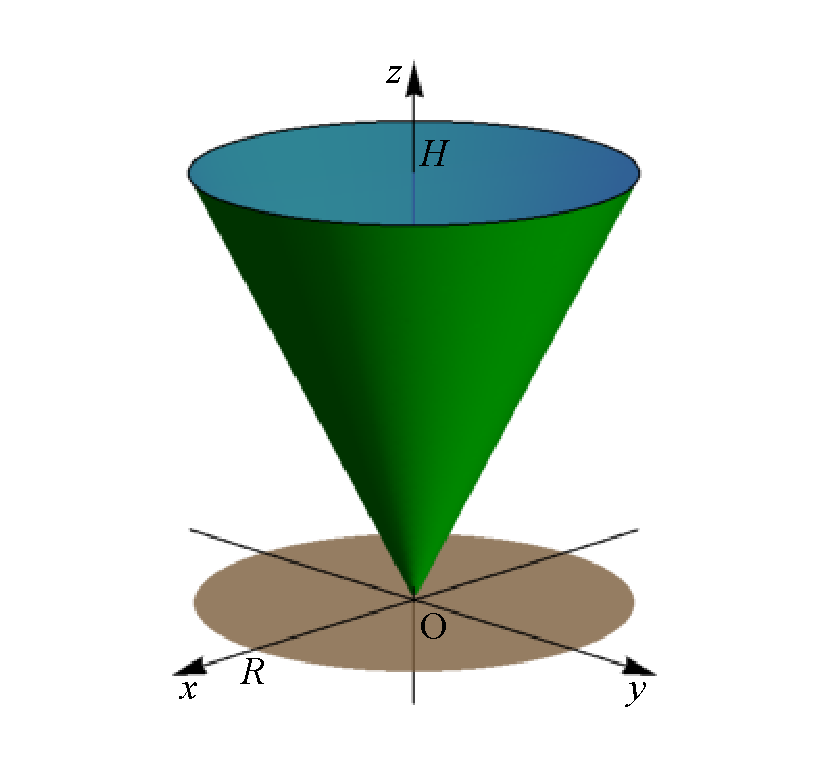
\includegraphics[height=0.7\textheight]{Figures21/Fig12-C-3.pdf}
\end{center}
\caption{第12章补充题 3.题图示}
\label{12-C-3}
\end{figure}

解:以该圆锥体的顶点为坐标原点,该圆锥体的旋转轴为$z$轴,建立空间直角坐标系,使该圆锥体在$xOy$平面上方,该圆锥体占据的空间区域可表示为$\Omega=\Set{(x,y,z)}{\frac HR\sqrt{x^2+y^2}\leqslant z\leqslant H,x^2+y^2\leqslant R^2}=\Set{(\theta,r,z)}{0\leqslant\theta\leqslant2\pi,0\leqslant r\leqslant R,\frac HRr\leqslant z\leqslant H}$根据对称性可知引力的$x$和$y$分量$F_x=F_y=0$,设该圆锥体的密度为$\rho$,则引力的$z$分量

$F_z=\varIIInt\Omega{\frac{G\rho m}{x^2+y^2+z^2}\frac z{\sqrt{x^2+y^2+z^2}}}xyz=\Int0{2\pi}{}\theta\Int0R{}r\Int{\frac HRr}H{\frac{G\rho m}{r^2+z^2}\frac z{\sqrt{r^2+z^2}}r}z\\
=2\pi G\rho m\Int0R{}r\Int{\frac HRr}H{\frac{rz}{(r^2+z^2)^{\frac32}}}z=2\pi G\rho m\Int0R{\frac12r\frac1{1-\frac32}(r^2+z^2)^{-\frac32+1}\big|_{\frac HRr}^H}r\\
=2\pi G\rho m\Int0R{r(\frac1{\sqrt{r^2+\frac{H^2}{R^2}r^2}}-\frac1{\sqrt{r^2+H^2}})}r=2\pi G\rho m\Int0R{(\frac1{\sqrt{1+\frac{H^2}{R^2}}}-\frac r{\sqrt{r^2+H^2}})}r\\
=2\pi G\rho m(\frac1{\sqrt{1+\frac{H^2}{R^2}}}r-\frac12\cdot\frac1{1-\frac12}\sqrt{r^2+H^2})\big|_0^R=2\pi G\rho m(\frac R{\sqrt{1+\frac{H^2}{R^2}}}-\sqrt{R^2+H^2}+H)\\
=2\pi G\rho m(H+\frac{R^2-R^2-H^2}{\sqrt{R^2+H^2}})=2\pi G\rho m(H-\frac{H^2}{\sqrt{R^2+H^2}})$,

故该圆锥体对位于其顶点处质量为$m$的质点的引力为$(0,0,2\pi G\rho m(H-\frac{H^2}{\sqrt{R^2+H^2}}))$.

(2)该圆锥体关于它的中心轴的转动惯量

$J_z=\varIIInt\Omega{(x^2+y^2)\rho}xyz=\Int0{2\pi}{}\theta\Int0R{}r\Int{\frac HRr}H{r^2\rho\cdot r}z=2\pi\rho\Int0R{r^3(H-\frac HRr)}r\\
=2\pi\rho(\frac14Hr^4-\frac15\frac HRr^5)\big|_0^R=2\pi\rho(\frac14HR^4-\frac15HR^4)=\frac1{10}\pi\rho HR^4$.

\item[9.]设一元函数$f$连续,$\Omega_t=\Set{(x,y,z)}{x^2+y^2\leqslant t^2,0\leqslant z\leqslant h}$. 令$F(t)=\IIInt{\Omega_t}{[z^2+f(x^2+y^2)]}V$,试求$\frac{\md F}{\md t}$和$\LIM t0\frac{F(t)}{t^2}$.

解:$F(t)=\varIIInt{\Omega_t}{[z^2+f(x^2+y^2)]}xyz=\Int0{2\pi}{}\theta\Int0t{}r\Int0h{[z^2+f(r^2)]r}z\\
=2\pi\Int0t{[\frac13rz^3+rf(r^2)z]\big|_0^h}r=2\pi\Int0t{[\frac13h^3r+hrf(r^2)]}r$,

$\therefore\frac{\mathrm dF}{\mathrm dt}=\frac{2\pi}3h^3t+2\pi htf(t^2)$,

$\therefore\LIM t0\frac1{t^2}F(t)=\LIM t0\frac{\frac{\mathrm dF}{\mathrm dt}}{2t}=\LIM t0\frac{2\pi[\frac13h^3t+htf(t^2)]}{2t}=\LIM t0\pi[\frac13h^3+hf(t^2)]=\frac\pi3h^3+\pi hf(0)$.

\item[10.]计算下列积分:\\
(1)$\IIInt\Omega{(ax+by+cz)^2}V$,其中$\Omega=\Set{(x,y,z)}{x^2+y^2+z^2\leqslant R^2}$;\\
(2)$\IIInt\Omega{(\frac{x^2}{a^2}+\frac{y^2}{b^2}+\frac{z^2}{c^2})}V$,其中$\Omega=\Set{(x,y,z)}{\frac{x^2}{a^2}+\frac{y^2}{b^2}+\frac{z^2}{c^2}\leqslant1}$.

解:(1)方法1:由对称性可知

$\IIInt\Omega{(ax+by+cz)^2}V=\IIInt\Omega{(a^2x^2+b^2y^2+c^2z^2+2abxy+2acxz+2bcyz)}V\\
=\IIInt\Omega{(a^2x^2+b^2y^2+c^2z^2)}V=(a^2+b^2+c^2)\IIInt\Omega{z^2}V\\
=(a^2+b^2+c^2)\varIIInt\Omega{r^2\cos^2\varphi\cdot r^2\sin\varphi}\theta\varphi r\\
=(a^2+b^2+c^2)\Int0{2\pi}{}\theta\Int0R{r^4}r\Int0\pi{\cos^2\varphi\sin\varphi}\varphi\\
=\frac25\pi R^5(a^2+b^2+c^2)(-\frac13\cos^3\varphi)\big|_0^\pi=\frac4{15}\pi R^5(a^2+b^2+c^2)$.

方法2:$\IIInt\Omega{(ax+by+cz)^2}V=\IIInt\Omega{(a^2x^2+b^2y^2+c^2z^2+2abxy+2acxz+2bcyz)}V\\
=\IIInt\Omega{(a^2x^2+b^2y^2+c^2z^2)}V=(a^2+b^2+c^2)\IIInt\Omega{z^2}V=\frac13(a^2+b^2+c^2)\IIInt\Omega{(x^2+y^2+z^2)}V\\
=\frac13(a^2+b^2+c^2)\Int0{2\pi}{}\theta\Int0\pi{}\varphi\Int0R{r^2\cdot r^2\sin\varphi}r=\frac23\pi(a^2+b^2+c^2)\Int0\pi{\sin\varphi}\varphi\Int0R{r^4}r\\
=\frac23\pi(a^2+b^2+c^2)(-\cos\varphi)\big|_0^\pi\frac15r^5\big|_0^R=\frac4{15}\pi R^5(a^2+b^2+c^2)$.

(2)令$\begin{cases}
x=au,\\
y=bv,\\
z=cw,
\end{cases}$则$\Omega=\Set{(u,v,w)}{u^2+v^2+w^2\leqslant1}$,

$\frac{\mathrm D(x,y,z)}{\mathrm D(u,v,w)}=\begin{vmatrix}
a&0&0\\
0&b&0\\
0&0&c
\end{vmatrix}=abc$,

$\therefore\IIInt\Omega{(\frac{x^2}{a^2}+\frac{y^2}{b^2}+\frac{z^2}{c^2})}V=\varIIInt\Omega{(u^2+v^2+w^2)|\frac{\mathrm D(u,v,w)}{\mathrm D(x,y,z)}|}uvw=abc\varIIInt\Omega{(u^2+v^2+w^2)}uvw\\
=abc\frac4{15}\pi 1^4(1^2+1^2+1^2)=\frac45\pi abc$.

\end{enumerate}
\end{document}